\documentclass[11pt, a4paper]{article}

\usepackage[T1]{fontenc}
\usepackage[utf8]{inputenc}
\usepackage{csquotes}
\usepackage{parskip}

\usepackage{bbm}
\usepackage{amsmath}
\usepackage{amssymb}
\usepackage{amsthm}
\usepackage{mathtools}
\usepackage{multirow}
\usepackage{makecell}
\usepackage{float}
\usepackage{caption}
\usepackage{subcaption}
\usepackage{enumitem}
\usepackage[hidelinks]{hyperref}
\usepackage{tikz}
\usetikzlibrary{positioning}
\usetikzlibrary{calc}
\usetikzlibrary{decorations.markings}
\usetikzlibrary{arrows.meta}
\usetikzlibrary{shapes.geometric}
% Algorithms
\usepackage[linesnumbered,ruled,vlined]{algorithm2e}
\SetKwInput{KwInput}{Input}
\SetKwInput{KwOutput}{Output}
\SetKw{KwContinue}{continue}
\SetKw{KwGoto}{go to}
\DontPrintSemicolon
%Define short commands for different letters
\foreach \x in {A,...,Z}{
\expandafter\xdef\csname b\x\endcsname{\noexpand\mathbb{\x}}
\expandafter\xdef\csname c\x\endcsname{\noexpand\mathcal{\x}}
\expandafter\xdef\csname f\x\endcsname{\noexpand\mathfrak{\x}}
}
% Math shortcuts
\newcommand{\mr}[1]{\mathrm{#1}}
\newcommand{\stackalign}[2]{\stackrel{\mathclap{#1}}{#2}}
\renewcommand{\bar}[1]{\overline{#1}}
\renewcommand{\hat}[1]{\widehat{#1}}
\newcommand{\floor}[1]{\lfloor #1 \rfloor}
\newcommand{\ceil}[1]{\lceil #1 \rceil}
\newcommand{\abs}[1]{\left\lvert#1\right\rvert}
\newcommand{\norm}[1]{\left\lVert#1\right\rVert}
\newcommand{\set}[1]{\{#1\}}
\renewcommand{\d}{\mathop{}\!\mathrm{d}}
\DeclareMathOperator{\Id}{Id}
\DeclareMathOperator{\im}{im}
\DeclareMathOperator{\Hom}{Hom}
\DeclareMathOperator{\End}{End}

\newenvironment{graph}[1][]{
	\begin{tikzpicture}[
		vertex/.style={circle,fill,inner sep=0,minimum size=5},
		dedge/.style={-Stealth},
		#1
	]
}{\end{tikzpicture}}

% Theorems, definitions, etc.
\newtheorem{theorem}{Theorem}[section]
\newtheorem{lemma}[theorem]{Lemma}
\newtheorem{cor}[theorem]{Corollary}
\newtheorem{prop}[theorem]{Proposition}
\newtheorem{conjecture}[theorem]{Conjecture}
\newtheorem*{claim}{Claim}
\newtheorem*{observation}{Observation}
\newtheorem*{utheorem}{Theorem}
\newtheorem*{uprop}{Proposition}
\theoremstyle{remark}
\newtheorem{remark}[theorem]{Remark}
\newtheorem*{uremark}{Remark}
\newtheorem{nexample}[theorem]{Example}
\newtheorem*{example}{Example}
\theoremstyle{definition}
\newtheorem{definition}[theorem]{Definition}
\newtheorem*{problem}{Problem}

\setcounter{section}{-1}

\title{Combinatorial Optimization}
\author{Dozent: Stephan Held}



\begin{document}
\maketitle
\tableofcontents
\clearpage

\section{Organization}
\begin{itemize}
	\item Prerequisites
	\begin{itemize}
		\item Basic knowledge of graph algorithms
		\item Linear Programming (LP Duality)
		\item Programming skills in C++
	\end{itemize}

	\item Exam
	\begin{itemize}
		\item Qualification requires 50\% of the points in theoretical \&
		programming exercises
		\item Oral exam
	\end{itemize}

	\item Books
	\begin{itemize}
		\item ''Combinatorial Optimization'', Korte \& Vygen
		\item ''Understanding \& Using Linear Programming'', B. Gärtner,
		J. Matouset
		\item Skript (theorems \& definitions)
		\item Further book recommendations are on the website
	\end{itemize}
\end{itemize}

\section{Matchings}
\subsection{Introduction}

\begin{definition}\
	\begin{enumerate}
		\item A \emph{matching} $M$ in a graph $G=(V,E)$ is a set of pairwise
		disjointed edges, i.e. they don't have a common endpoint.

		$\nu(G)\coloneqq$ max. cardinality of a matching in $G$

		\item An \emph{edge cover} $C$ of a graph $G=(V,E)$ is a subset of $E$ s.t.
		$V=\bigcup_{e\in C}e$.

		$\zeta(G) \coloneqq$ min. cardinality of an edge cover in $G$

		\item A matching is called \emph{perfect} (or \emph{1-factor}) if it is an
		edge cover

		\item $v\in V$ with $v\in e\in M$ is called \emph{$M$-covered}

		\item $v\in V$ is called \emph{$M$-exposed} if it is not
		$M$-covered
	\end{enumerate}
\end{definition}

\begin{definition}\
	\begin{enumerate}
		\item A \emph{stable set} (independent set) $S$ is a set of pairwise
		non-adjacent vertices.

		$\alpha(G)\coloneqq$ max. cardinality of a stable set

		\item A \emph{vertex cover} $C$ is a subset of $V$ s.t.
		$E=\bigcup_{\{x,y\}\in E,\ x\in G}\{x,y\}$

		$\tau(G)\coloneqq$ min. cardinality of a vertex cover
	\end{enumerate}
\end{definition}

\begin{lemma}\
	\begin{enumerate}
		\item $\alpha(G)+\tau(G) = \abs{V}$
		\item $\nu(G) + \zeta(G) = \abs{V}$ if $G$ has no isolated vertices
		\item $\zeta(G)=\alpha(G)$ if $G$ is bipartite and has no isolated
		vertices
	\end{enumerate}
\end{lemma}

\begin{problem}{Cardinality Matching Problem}\\
Input: Graph $G=(V,E)$ \\
Task: Find a maximum cardinality matching
\end{problem}

\begin{problem}{Maximum Weight Matching Problem (MWMP)}\\
Input: Graph $G$, $c:E\to \bR$ \\
Task: Find a matching $M$ maximizing $c(M)$
\end{problem}

\begin{problem}{Minimum Weight Perfect Matching (MWPMP)}\\
Input: Graph $G$, $c:E\to\bR$\\
Task: Find a perfect matching of minimum weight or decide that no
perfect matching exists in $G$
\end{problem}

\begin{lemma}
	The MWMP is equivalent to the MWPMP (i.e. there exists a transformation
	with linear complexity)
\end{lemma}
\begin{proof}
	Given a MWPMP instance $(G,c)$, define $c':=K-c$
	($K\coloneqq 1+\sum_{e\in E}\abs{c(e)}$). \\
	$\Rightarrow$ Any maximum weight matching is a maximum cardinality
	matching

	Given a MWMP instance $(G,c)$, define $G'$ as 2 copies of $G$ where
	the 2 copies of a vertex are joined by an edge. \\ $\Rightarrow$ $G'$
	has a perfect matching. Define:
	\[c'(e)\coloneqq \begin{cases}
			-c(e) \quad & \text{if $e$ is in the first copy} \\
			0           & \text{else}
		\end{cases}\]
	A minimum weight perfect matching in $G'$ gives us a maximum weight
	matching in $G$.
\end{proof}

\begin{definition}
	Let $G=(V,E)$ be a graph and $M\subseteq E$ a matching in $G$.
	A path $P$ is \emph{$M$-alternating} if its edges are alternatingly
	in and not in $M$. If both end points of this path are $M$-exposed,
	$P$ is an \emph{$M$-augmenting} path.
\end{definition}

\begin{lemma}
	Given a matching $M$ in $G$ and an inclusion-wise maximal
	$M$-alternating path $P$,
	\[M\Delta P\coloneqq M\setminus P\cup P\setminus M\]
	is a matching. If $P$ is $M$-augmenting, then $\abs{M\Delta
			P}=\abs{M}+1$.
\end{lemma}

\begin{theorem}[Petersen 1891, Berge 1957]{Augmenting Path Theorem}
	Given a graph $G=(V,E)$ and a matching $M$ in $G$:
	\[\abs{M}=\nu(G) \Leftrightarrow \not\exists \text{$M$-augmenting
			path $P$ in $G$}\]
\end{theorem}
\begin{proof}\
	\begin{enumerate}
		\item[''$\Rightarrow$'':] Clear
		\item[''$\Leftarrow$'':] Assume there exists a matching $M'$
		with $\abs{M'}>\abs{M}$. Let $G'\coloneqq (V, M\Delta M')$. \\
		$\Rightarrow$ $\abs{\delta_{G'}(v)}\leq 2\ \forall v\in V$ \\
		$\Rightarrow G'$ is the union of disjoint circuits and paths \\
		$\Rightarrow$ all circuits are even and have the same number of edges
		from $M$ and $M'$ \\
		$\Rightarrow \exists$ a path $P$ in $G'$ starting and ending with an
		edge in $M'$ \\
		$\Rightarrow P$ is an alternating path
	\end{enumerate}
\end{proof}

\subsection{Bipartite Matching}

\begin{theorem}[König 1931]\label{thm:koenig-bipartite}
	If $G$ is bipartite, then $\nu(G)=\tau(G)$
\end{theorem}
\begin{proof}
	Add vertices $s$ and $t$ edges between them to all vertices of the
	respective partition. Direct all edges from $s$ to $t$. Then
	$\nu(G)$ is maximum number of disjoint $s$-$t$-paths. Menger
	$\Rightarrow$ This is equal to the minimum number of vertices that
	disconnect $t$ from $s$.
\end{proof}

\begin{figure}
	\centering
	\begin{graph}
		\node[vertex] (s) at (-2,0) {};
		\node[vertex] (a1) at (0,1) {};
		\node[vertex] (a2) at (0,0) {};
		\node[vertex] (a3) at (0,-1) {};
		\node[vertex] (b1) at (2,0.5) {};
		\node[vertex] (b2) at (2,-0.5) {};
		\node[vertex] (t) at (4,0) {};
		\node (sl) [above=0 of s] {$s$};
		\node (tl) [above=0 of t] {$t$};
		\node (al) at (0,1.5) {$A$};
		\node (bl) at (2,1.5) {$B$};

		\draw[dedge] (s) -- (a1);
		\draw[dedge] (s) -- (a2);
		\draw[dedge] (s) -- (a3);
		\draw[dedge] (a1) -- (b1);
		\draw[dedge] (a1) -- (b2);
		\draw[dedge] (a2) -- (b2);
		\draw[dedge] (a3) -- (b2);
		\draw[dedge] (b1) -- (t);
		\draw[dedge] (b2) -- (t);
	\end{graph}
	\caption{Example of the construction in Theorem \ref{thm:koenig-bipartite}}
\end{figure}

\begin{theorem}[Hall 1935]
	Let $G=(A\dot\cup B, E)$ be a bipartite graph. Then:
	\[
		G\text{ has a matching covering $A$}\Leftrightarrow
		\abs{\Gamma(X)} \geq \abs{X} \quad\forall X\subseteq A
	\]
\end{theorem}

\begin{cor}{Marriage Theorem}
	\[
		\abs{\Gamma(X)}\geq\abs{X}\ \forall X\subseteq A\text{ and }
		\abs{A}=\abs{B} \Leftrightarrow G \text{ has a perfect matching}
	\]
\end{cor}

% Numbering is broken in the lecture
\stepcounter{theorem}

\begin{definition}
	The MWPMP for bipartite graphs is called \emph{Assignment Problem}.
\end{definition}

\begin{theorem}
	The Assignment Problem can be solved in time $O(nm+n^2\log m)$.
\end{theorem}
\begin{proof}
	Use the Successive Shortest Paths algorithm in an auxiliary graph.
\end{proof}

\subsection{The Tutte Matrix \& Randomized Matching}

\begin{definition}
	Let $G$ be a simple, undirected graph. Let $G'$ be an orientation
	of $G$ and $(X_e)_{e\in E(G)}$. The \emph{Tutte matrix} is defined as
	\[T_G(X)\coloneqq (t^*_{vw})_{v,w\in V(G)}\]
	where
	\[
		t^*_{vw}\coloneqq \begin{cases}
			X_{\{v,w\}} \quad & \text{if $(v,w)\in E(G')$} \\
			-X_{\{v,w\}}      & \text{if $(w,v)\in E(G')$} \\
			0                 & \text{else}
		\end{cases}
	\]
\end{definition}

\begin{remark}
	$T_G(X)$ is shew-symmetric (i.e. $T_G(X)=-(T_G(X))^t$).
	$\mathrm{rank}(T_G(X))$ is independent of the orientation of $G$.
	$\det(T_G(X))$ is a polyomial in $X$.
\end{remark}

\begin{theorem}[Tutte]
	A simple graph $G$ has a perfect matching $\Leftrightarrow
		\det(T_G(X))\neq0$
\end{theorem}
\begin{proof}
	Let $V(G)=\{v_1,\ldots,v_n\}$ and $S_n$ be the permutation group.
	\begin{align*}
		\det T_G(X)=\sum_{\pi\in S_n}\mathrm{sgn}\pi\cdot \prod_{i=1}^n
		t_{v_i,v_{\pi(i)}}^*
	\end{align*}
	Let $S_n'\coloneqq\{\pi\in S_n\ |\ \prod_{i=1}^n
		t_{v_i,v_{\pi_i}}^*\neq0\}$. Each $\pi\in S_n$ corresponds to a
	digraph $H_\pi\coloneqq (V(G), \{(v_i,v_{\pi(i)})\ |\ i\in [n]\footnote{
			This is an abbreviation for $\{1,\ldots,n\}$.
		}\})$.
	We have $\abs{\delta^+(v)=1=\abs{\delta^-(v)}}\ \forall v\in V(H_\pi)$
	$\Rightarrow H_\pi$ is the union of disjoint circuits.
	If $\pi\in S_n'$, then $H_\pi\subset \stackrel{\Leftrightarrow}{G'}$.

	If there exists $\pi\in S_n'$ s.t. $H_\pi$ is a collection of even
	circuits, then this immediately yields a perfect matching in $G$
	(using every second edge of each circuit).

	Otherwise, $\forall \pi\in S_n'$, $H_\pi$ contains an odd circuit.
	Let $r(\pi)\in S_n'$ arise from $\pi$ by reversing edges on the
	unique odd circuit containing a vertex with minimum index
	$\Rightarrow r(r(\pi))=\pi$ and
	$\mathrm{sgn}(\pi)=\mathrm{sgn}(r(\pi))$. The second part is true
	since for reversing an odd cycle, we need an even number of swaps.
	Let $v_{i_1},\ldots,v_{i_{2k+1}}$ be the ''first'' odd circuit. Then
	$r(\pi)$ is attained by $2k$ swaps: For $j=1,\ldots,k$ swap
	$(\pi(i_{2j-1}), \pi(i_{2k}))$ and $(\pi(i_{2j}), \pi(i_{2k+1}))$.

	$\prod_{i=1}^n t_{v_iv_{\pi(i)}}^*=-\prod_{i=1}^nt_{v_iv_{r(\pi(i))}}^*$
	since there is an odd number of sign changes to $t^*$.
	$\Rightarrow \det(T_G(X))=0$. We have shown that if $G$ has no perfect
	matching, then $\det T_G(X)=0$.

	Assume that $G$ has a perfect matching $M$. Define $\pi$ as
	$\pi(i)=j, \pi(j)=i$ where $\{i,j\}\in M$. $\Rightarrow \prod_{i=1}^n
		t_{v_iv_{\pi(i)}}^*=\prod_{e\in M}-X_e^2$ cannot be canceled out. In
	particular, $\det T_G(X)\neq0$.
\end{proof}

\begin{remark}
	Picking $X'\in [0,1]^{E(G)}$ at random, we almost surely have (since
	the zero set of a non-zero polynomial is a set of measure zero):
	\[\det T_G(X')\neq0 \Leftrightarrow G\text{ has a perfect matching}\]
\end{remark}

\begin{theorem}[Lovász 1979]
	Let $G$ be a simple graph and $X\in [0,1]^{E(G)}$ chosen randomly.
	Then almost surely $\mathrm{rank}(T_G(X))=2\nu(G)$.
\end{theorem}

\subsection{Tutte's Matching Theorem}
Let $X\subseteq V(G)$. $G-X$ consists of even and odd (in terms of
the number of vertices) connected components. We define $q_G(X)$ to
be the number of odd components in $G-X$.

\begin{figure}[tbh]
	\centering
	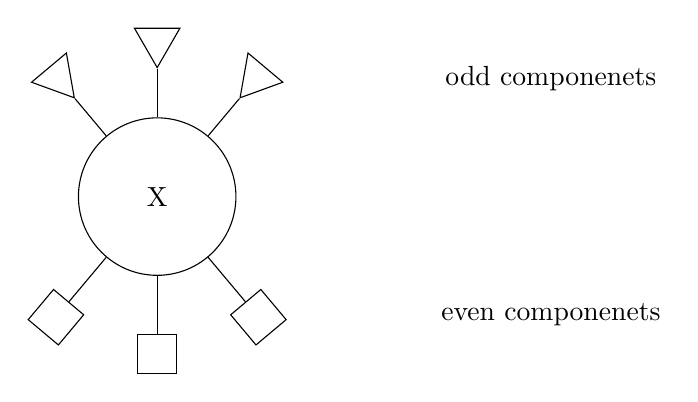
\begin{tikzpicture}
		\node[draw, circle, minimum size =2cm] (X) at (0,0) {X};
		\begin{scope}[every node/.style={draw, isosceles triangle, isosceles triangle apex angle=60, minimum size=0.5cm}, node distance = 2cm]
			\node[rotate=270] (a) [left of=X]  {};
			\node[rotate=230] (b) [left of =X]  {};
			\node[rotate=310] (c) [left of =X]  {};
		\end{scope}
		\begin{scope}[every node/.style={draw, minimum size=0.5cm}, node distance = 2cm]
			\node[rotate=270] (d) [right of=X]  {};
			\node[rotate=230] (e) [right of =X]  {};
			\node[rotate=310] (f) [right of =X]  {};
		\end{scope}
		\draw (X) -- (a);
		\draw (X) -- (b);
		\draw (X) -- (c);
		\draw (X) -- (d);
		\draw (X) -- (e);
		\draw (X) -- (f);
		\node (even) at (5,-1.5) {even componenets};
		\node (odd) at (5,1.5) {odd componenets};
	\end{tikzpicture}
\end{figure}

\begin{definition}
	A graph $G$ satisfies the \emph{Tutte Condition} if $q_G(X)\leq\abs{X}$
	for all $X\subseteq V(G)$. $\emptyset\neq X\subseteq V(G)$ is called
	\emph{barrier} if $q_G(X)=\abs{X}$.
\end{definition}

\begin{prop}\label{prop:tutte-even}
	For any graph $G$ and any $X\subseteq V(G)$:
	\[q_G(X)-\abs{X} \equiv \abs{V(G)}\mod 2\]
\end{prop}

\begin{definition}
	A graph $G$ is \emph{factor-critical} if $G-v$ has a perfect matching
	for all $v\in V(G)$. A matching is called \emph{near-perfect} if it
	covers $\abs{V(G)}-1$ vertices.
\end{definition}

\begin{prop}\label{prop:factor-critical-conn}
	If $G$ is factor-critical, then it is connected.
\end{prop}

\begin{theorem}[Tutte 1947]
	A graph $G$ has a perfect matching $\Leftrightarrow$ Tutte Condition
	holds (i.e. $q_G(X)\leq\abs{X}\ \forall X\subseteq V(G)$)
\end{theorem}
\begin{proof}\
	\begin{enumerate}
		\item[''$\Rightarrow$'':] Clear
		\item[''$\Leftarrow$'':] We proceed by induction on $\abs{V(G)}$.
		The case $\abs{V(G)}=2$ is clear.

		Generally, if the Tutte Condition holds, then $\abs{V(G)}$ must be
		even (pick $X=\emptyset$). Proposition \ref{prop:tutte-even}
		$\Rightarrow q_G(X)-\abs{X}$ is even. Every $x\in V(G)$ induces a
		barrier $\{x\}$. Let $X$ be a maximum barrier. Then $G-X$ doesn't
		have any even components (since otherwise a single vertex of such a
		component could be added to $X$).

		\textbf{Claim:} Each odd component is factor-critical. \\
		Let $C$ be an odd component in $G-X$, $v\in V(C)$. Assume that $C-v$
		does not have a perfect matching. Induction Hypothesis $\Rightarrow$
		$C-v$ violates Tutte Condition. \\
		$\Rightarrow \exists Y\subseteq V(C-v): q_{C-v}(Y)>\abs{Y}$ \\
		$\stackrel{\ref{prop:tutte-even}}{\Rightarrow} q_{C-v}(Y)\geq \abs{Y}+2$ \\
		Observe $X\cap\{v\}=Y\cap\{v\}=X\cap Y=\emptyset$:
		\begin{align*}
			q_G(X\cup Y\cup\{v\}) & =q_G(X)-1+q_C(Y\cup\{v\}) \\
			                      & =\abs{X}-1+q_{C-v}(Y)     \\
			                      & \geq\abs{X}-1+\abs{Y}+2   \\
			                      & =\abs{X\cup Y}+1          \\
			                      & =\abs{X\cup Y\cup\{v\}}
		\end{align*}
		$\Rightarrow X\cup Y\cup\{v\}$ is a barrier \\
		$\Rightarrow$ Claim

		Let $G'$ arise from $G$ by contracting each odd component into a
		single vertex. We have $V(G')=X\dot\cup Z$ and $G'$ is bipartite. We
		have to show that $G'$ has a perfect matching. If not, then $\exists
			A\subseteq Z: \abs{\Gamma_{G'}(A)}<\abs{A}$ \\ $\Rightarrow
			q_G(\Gamma_{G'}(A))\geq \abs{A}>\abs{\Gamma_{G'}(A)}$ which
		contradicts the Tutte Condition.
	\end{enumerate}
\end{proof}

\begin{theorem}[Berge 1958]\label{tutte-berge}
	\[\abs{V(G)}=2\nu(G)+\max_{X\subseteq V(G)}(q_G(X)-\abs{X})\]
\end{theorem}
\begin{proof}
	For $X\subseteq V(G)$, any matching has at least $q_G(X)-\abs{X}$
	uncovered vertices, so ''$\geq$'' holds.

	For the other inequality, add $k\coloneqq\max_{X\subseteq V(G)}
		(q_G(X)-\abs{X})$ new vertices and connect them to all existing
	vertices, yielding a new graph $H$.

	We claim that $H$ has a perfect matching. This then implies:
	\[2\nu(G)+k\geq 2\nu(H)-k =\abs{V(H)}-k=\abs{V(G)}\]
	Assume that $H$ does not have a perfect matching. Then by Tutte's
	Theorem, there exists $Y\subseteq V(H)$ with $q_H(Y)>\abs{Y}$. By
	\ref{prop:tutte-even}, $k\equiv \abs{V(G)}\mod 2$, therefore
	$\abs{V(H)}$ is even, so $Y\neq\emptyset$. $Y$ must contain all new
	vertices, otherwise $H-Y$ would be connected\footnote{ Note that $Y$
		cannot contain all old vertices, since otherwise $q_H(Y)<\abs{Y}$. }
	and $q_H(Y)\leq 1\leq\abs{Y}$. \\
	\[\Rightarrow q_G(Y\cap\abs{V(G)})=q_H(Y)>\abs{Y}=\abs{Y\cap V(G)}+k\]
	which is a contradiction to the choice of $k$.
\end{proof}

\subsection{Ear Decompositions of Factor-Critical Graphs}
\begin{definition}
	Let $G$ be a graph. An \emph{ear decomposition} of $G$ is a sequence
	$r,P_1,\ldots,P_k$ with $G=(r,\emptyset)+P_1+\ldots+P_k$ such that each
	$P_i$ is either a path with exactly the endpoints located in
	$\set{r}\cup\bigcup_{j\in[i-1]}V(P_j)$ or a circuit where exactly one
	of the vertices belongs to $\set{r}\cup\bigcup_{j\in[i-1]}V(P_j)$.

	$P_1,\ldots,P_k$ are called \emph{ears}. If $\abs{V(P_1)}\geq 3$ and
	$P_2,\ldots,P_k$ are paths we call it a \emph{proper} ear decomposition.
\end{definition}

% Numbering in the lecture is broken
\stepcounter{theorem}

\begin{theorem}[Whitney 1932]
	Let $G$ be an undirected graph. Then:
	\[G\text{ 2-connected}\Leftrightarrow
		G\text{ has a proper ear decomposition}\]
\end{theorem}

\begin{definition}
	An ear decomposition is \emph{odd} if every ear has odd length (in terms
	of the number of edges).
\end{definition}

\begin{theorem}
	Let $G$ be an undirected graph. Then
	\[G\text{ factor-critical}
		\Leftrightarrow G\text{ has an odd ear decomposition}\]
	The first vertex $r$ of the ear decomposition can be chosen
	arbitrarily.
\end{theorem}
\begin{proof}\
	% TODO : two figures within proof
	\begin{enumerate}
		\item[''$\Leftarrow$'':]
		Let $G$ be a graph with an odd ear decomposition $r,P_1,\ldots,P_k$.
		$P_1$ is an odd circuit, so it is factor-critical. We use induction on the
		number of ears. Let $P$ be the last ear and $G'$ be $G$ before adding $P$.
		By the induction hypothesis, $G'$ is factor-critical.
		Given $v\in V(G)$, we have to show that $G-v$ has a perfect matching.
		\begin{enumerate}
			\item[Case 1:] $v\in V(G')$. Then $G'-v$ has a perfect matching. Adding
			every second edge of $P$ (excluding the endpoints) to it, yields a
			perfect matching of $G-v$.

			\item[Case 2:] $v\in V(G)\setminus V(G')$. Let $x,y$ be the endpoints of
			$P$. Without loss of generality let $P_{[v,x]}$ be even. There exists
			a perfect matching in $G'-x$. Together with every second edge of
			$P_{[v,y]}$ and $P_{[v,x]}$ this is a perfect matching in $G-v$.
		\end{enumerate}

		\item[''$\Rightarrow$'':]
		Let $r\in V(G)$ be any vertex. Let $M$ be a perfect matching in $G-r$.
		Suppose we have an odd ear decomposition for $G'\subseteq G$ with
		$r\in V(G')$ and $M\cap E(G')$ is a near-perfect matching in $G'$ (i.e.
		all vertices in $G'$ except for $r$ are matched with other vertices in $G'$).

		If $G'\neq G$, there is an edge $\set{x,y}\in E(G)\setminus E(G')$
		with $x\in V(G')$ (by Proposition \ref{prop:factor-critical-conn}).
		If $y\in V(G')$, then $\set{x,y}$ can be chosen as the next ear.
		Otherwise, we construct an $M$-alternating odd ear, starting with
		$\set{x,y}$: Let $N$ be a matching in $G-y$. $M\Delta N$ contains a
		$y$-$r$-path $P$. Let $w$ be the first vertex in $P\cap V(G')$. $w$
		is $M$-exposed in $P_{[y,w]}$, $y$ is $N$-exposed in $P_{[y,w]}$.
		Therefore $P_{[y,w]}$ is even and together with $\set{x,y}$ it forms
		an $M$-alternating odd ear.

		Inductively, this argument yields an odd ear decomposition.
	\end{enumerate}
\end{proof}

\begin{definition}
	Let $G$ be factor-critical and $M$ a near-perfect matching.
	An $M$-alternating ear decomposition is an odd ear decomposition
	such that each ear is an $M$-alternating path or circuit $C$ with:
	\[\abs{E(C)\cap M}=\abs{E(C)\setminus M}-1\]
\end{definition}

\begin{cor}
	For any factor-critical graph $G$ and any near-perfect matching $M$ in $G$,
	there exists in $M$-alternating ear decomposition of $G$.
\end{cor}

\begin{definition}
	Let $G$ be factor-critical, $M$ a near-perfect matching and
	$r,P_1,\ldots,P_k$ an $M$-alternating ear decomposition of $G$.
	$\mu,\varphi: V(G)\to V(G)$ are \emph{associated with the ear
		decomposition} if:
	\begin{itemize}
		\item $\set{x,y}\in M\Rightarrow \mu(x)=y$
		\item $\set{x,y}\in E(P_i)\setminus M$ and $x\notin\set{r}
			\cup\bigcup_{j\in [i-1]}V(P_j)$

		$\Rightarrow \varphi(x)=y$
		\item $\mu(r)=\varphi(r)=r$
	\end{itemize}
\end{definition}

\begin{prop}\label{lemma:ear-decomp-repr}
	Let $G$ be a factor-critical graph and $\mu,\varphi$ functions associated
	with an $M$-alternating ear decomposition. Then this ear decomposition is
	unique up to the order of the ears. The Ear-Decomposition-Algorithm
	(algorithm \ref{alg:ear-decomp})
	correctly determines an explicit list of the ears in linear time.
\end{prop}
\begin{proof}
	Step 3 determines ears uniquely. The algorithm clearly runs in linear
	time.
\end{proof}

\begin{algorithm}[htbp]
	\caption{Ear Decomposition Algorithm}
	\label{alg:ear-decomp}
	\KwInput{Factor-critical graph $G$, functions $\mu,\varphi$ associated
		with an $M$-alternating ear decomposition}
	\KwOutput{An $M$-alternating ear decomposition $r,P_1,\ldots,P_k$}

	$X\coloneqq\set{r}$ where $r$ is the vertex with $\mu(r)=r$\;
	$k\coloneqq0$, $S\coloneqq$ empty stack\;
	\While{$X\neq V(G)$}{
		\If{$S$ is non-empty}{
			Let $v\in V(G)\setminus X$ be an endpoint of the topmost element of the
			stack\;
		}\Else{
			Choose $v\in V(G)\setminus X$ arbitrarily\;
		}
		$x\coloneqq v,\ y\coloneqq \mu(v),\ P\coloneqq (\set{x,y},\set{\set{x,y}})$\;
		\While{$\varphi(\varphi(x))=x$}{
			$P\coloneqq P+\set{x,\varphi(x)}+\set{\varphi(x),\mu(\varphi(x))}$\;
			$x\coloneqq\mu(\varphi(x))$\;
		}
		\While{$\varphi(\varphi(y))=y$}{
			$P\coloneqq P+\set{y,\varphi(y)}+\set{\varphi(y),\mu(\varphi(y))}$\;
			$y\coloneqq\mu(\varphi(y))$\;
		}
		$P\coloneqq P+\set{x,\varphi(x)}+\set{y,\varphi(y)}$\;
		$P$ is the ear containing $y$ as an inner vertex. Put $P$ on $S$.\;
		\While{Both endpoints of the topmost element $P$ of the stack $S$ are in
			$X$}{
			Delete $P$ from $S$\;
			$k\coloneqq k+1,\ P_k\coloneqq P,\ X\coloneqq X\cup V(P)$\;
		}
	}
	\ForAll{$\set{y,z}\in E(G)\setminus (E(P_1)\cup\ldots\cup E(P_k))$}{
		$k\coloneqq k+1,\ P_k\coloneqq (\set{y,z},\set{\set{y,z}})$\;
	}
	\KwRet{$r,P_1,\ldots,P_k$}
\end{algorithm}

\begin{lemma}\label{lemma:factor-critical-alt-path}
	Let $G$ be factor-critical and $\mu,\varphi$ associated with an
	$M$-alternating ear decomposition. Then the maximal path given by the
	initial sequence
	\begin{equation}\label{eq:ear-alt-path}
		x,\mu(x),\varphi(\mu(x)),\mu(\varphi(\mu(x))),\ldots
	\end{equation}
	defines an $M$-alternating $x$-$r$-path of even length.
\end{lemma}

\begin{figure}
	\centering
	\begin{graph}
		\node[vertex] (a) at (0,0) {};
		\node[vertex] (b) at (0,1) {};
		\node[vertex] (c) at (0,2) {};
		\node[vertex] (d) at (2,0) {};
		\node[vertex] (e) at (2,1) {};
		\node[vertex] (f) at (2,2) {};
		\node[vertex] (r) at (4,1) {};
		\node (rl) [above of =r, node distance =0.5cm] {r};

		\draw[dedge] (a) -- (b);
		\draw[dedge] (b) -- (c);
		\draw[dedge] (d) -- (r);
		\draw[dedge] (e) -- (r);
		\draw[dedge] (f) -- (r);
		\draw[dedge] (c) to[in=140,out=220] (a);
		\draw[double] (a) -- (d);
		\draw[double] (b) -- (e);
		\draw[double] (c) -- (f);

		\node (x) at (7,2) {x};
		\node (phi) at (9,2) {$\varphi(x)$};
		\draw[dedge] (x) -- (phi);
		\node[vertex] (g) at (7,0) {};
		\node[vertex] (h) at (9,0) {};
		\draw[double] (g) to (h);
		\node (M) at (8,0.3) {M-edge};
	\end{graph}
	\caption{
		Counter example for the reverse implication of lemma
		\ref{lemma:factor-critical-alt-path}
	}
\end{figure}

% Lecture 4, 27.10.22
\begin{proof}
	We proceed by induction on the number of ears. Let $x\in
		V(G)\setminus\set{r}$ and $P_i$ be the ear containing $x$.
	A subsequence of (\ref{eq:ear-alt-path}) is a subpath $Q$ of $P_i$ from
	$x$ to $y\in\set{r}\cup\bigcup_{j\in[i-1]}V(P_j)$. $Q$ starts with a
	matching edge and ends with a non-matching edge, so it has even length.
	If $y=r$, we are done, otherwise the statement follows from the induction
	hypothesis.
\end{proof}

\subsection{Edmond's Matching Algorithm}
\begin{definition}
	Let $G$ be a graph, $M$ a matching in $G$. A \emph{blossom} in $G$
	with respect to $M$ is a factor-critical subgraph $B$ of $G$ such that
	$\abs{M\cap E(B)}=\frac{\abs{V(B)}-1}{2}$. The vertex $r\in V(B)$ that is
	exposed by $M\cap E(B)$ is called the \emph{base} of $B$.
\end{definition}

\begin{definition}
	Let $G$ be a graph, $M$ a matching in $G$, $B$ a blossom and $Q$ a
	$M$-alternating $v$-$r$-path of even length from $v\in V(G)$ that is
	$M$-exposed to the base $r$ of $B$. Additionally, let
	$E(Q)\cap E(B)=\emptyset$. $B+Q$ is called an \emph{$M$-flower}.
\end{definition}

\begin{lemma}
	Let $G$ be a graph, $M$ a matching in $G$. Suppose there is a $M$-flower
	$B+Q$. Let $G',M'$ result from $G$ and $M$ by contracting $V(B)$ into
	a single vertex. Then:
	\[
		M\text{ maximum matching in $G$} \Leftrightarrow
		M'\text{ maximum matching in $G'$}
	\]
\end{lemma}
\begin{proof}\
	\begin{enumerate}
		\item[''$\Leftarrow$'':]
		Assume that $M$ is not maximum in $G$. $N\coloneqq M\Delta E(Q)$
		is a matching with $\abs{N}=\abs{M}$. \\
		$\Rightarrow \exists N$-augmenting path $P$ in $G$. At least one endpoint
		$x$ of $P$ is not in $V(B)$ (since $B$ contains only one $N$-exposed
		vertex). If $P$ and $B$ are disjoint, let $y$ be the other
		endpoint of $P$. Otherwise, let $y$ be the first vertex on $P$ in $B$.
		$P'\coloneqq P_{[x,y]}$ is an $N'$-augmenting path in $G'$, so
		$\abs{N'}=\abs{M'}<\mu(G')$.

		\item[''$\Rightarrow$'':]
		Assume that $M'$ is not maximum in $G'$, so there exists a matching $N'$
		in $G'$ with $\abs{N'}>\abs{M'}$. Let $N_0$ arise from $N'$ in $G$, then
		$N_0$ contains $\leq 1$ vertex from $V(B)$. Since $B$ is factor-critical,
		$N_0$ can be extended by $k\coloneqq\frac{\abs{V(G)}-1}{2}$ edges to a
		matching $N$ in $G$. We have
		\[\abs{N}=\abs{N_0}+k=\abs{N'}+k>\abs{M'}+k=\abs{M}\]
		so $M$ is not maximum.
	\end{enumerate}
\end{proof}

\stepcounter{theorem}
\begin{lemma}
	Let $G$ be a graph, $M$ a matching in $G$. $X\subseteq V(G)$ is the set
	of exposed vertices. We can find a shortest $M$-alternating $X$-$X$-walk
	of positive length in $O(\abs{E(G)})$ time.
\end{lemma}
\begin{proof}
	Define $D\coloneqq (V(G), A)$ where:
	\[
		A\coloneqq\set{(u,v)\ |\ \exists
			x\in V(G): \set{u,x}\in E(G), \set{x,v}\in M}
	\]
	A shortest $X-\Gamma_G(X)$-path in $D$ corresponds to a shortest
	$X$-$X$-walk in $G$.
\end{proof}

\begin{theorem}\label{thm:augmenting-path-blossom}
	Let $P=v_0,\ldots,v_t$ be a shortest $M$-alternating $X$-$X$-walk in $G$.
	Then either
	\begin{itemize}
		\item $P$ is an $M$-augmenting path \emph{or}
		\item $v_0,\ldots,v_j$ is an $M$-flower for some $j\leq t$.
	\end{itemize}
\end{theorem}
\begin{proof}
	If $P$ is not a path, choose $i<j$ such that $v_i=v_j$ and $j$ minimal.
	Then $v_0,\ldots,v_{j-1}$ are distinct vertices. If $j-i$ is even,
	deleting $v_{i-1},\ldots,v_j$ from $P$ yields a shorter walk, so $j-i$
	is odd.
	\begin{enumerate}
		\item[Case 1:] $j$ is even. Then $i$ is odd and therefore $v_{i+1}=v_{j-1}$
		must be the matching mate of $V_i=v_j$ which contradicts the
		minimality of $j$.
		\item[Case 2:] $j$ is odd. Then $i$ is even, so $v_0,\ldots,v_i$ is an
		$M$-alternating path of even length and $v_i,\ldots,v_j$ is an
		$M$-alternating odd circuit, i.e. a blossom.
	\end{enumerate}
\end{proof}

\begin{algorithm}
	\caption{Edmond's Augmenting Path Search}
	\KwInput{Graph $G$, matching $M$}
	\KwOutput{An $M$-augmenting path (if one exists)}
	$X\coloneqq$ set of exposed vertices\;
	\If{$\exists M$-alternating $X$-$X$-walk of positive length}{
		$P=v_0,\ldots,v_t\coloneqq$ a shortest such walk\;
		\If{$P$ is a path}{
			\KwRet{$P$}\;
		}\Else{
			Choose $j$ as in Theorem \ref{thm:augmenting-path-blossom}\;
			$v_0,\ldots,v_j$ is an $M$-flower with blossom $B$\;
			Recurse on $G/B$\;
			Augment an $M/B$-augmenting path in $G/B$ to an $M$-augmenting
			path $P'$ in $G$\;
			\KwRet{$P'$}\;
		}
	}\Else{
		$\not\exists M$-augmenting path\;
	}
\end{algorithm}

\begin{theorem}
	Given a graph $G$, a maximum cardinality matching can be found in time
	$O(n^2m)$ where $n\coloneqq\abs{V(G)}, m\coloneqq\abs{E(G)}$
\end{theorem}
\begin{proof}
	Start with $M=\emptyset$ and iteratively find $M$-augmenting path $P$,
	set $M\coloneqq M\Delta E(P)$. If no such path exists, then $M$ is
	maximum. $P$ can be found in time $O(mn)$\footnote{
		Here, $m$ is the time required for finding a walk and the recursion
		depth is bounded by $n$.
	}. Since $M$ is maximum after at most $\frac{n}{2}$ augmentation, we have
	total running time $O(n^2m)$.
\end{proof}

\subsubsection{Growing forest\texorpdfstring{ - $O(n^3)$}{}}
\begin{definition}
	Let $G$ be a graph, $M$ a matching in $G$. An \emph{alternating forest}
	with respect to $M$ in $G$ is a forest $F$ in $G$ where:
	\begin{itemize}
		\item $V(F)$ contains all $M$-exposed vertices, each tree of $F$
		contains exactly one exposed vertex, its \emph{root}.
		\item We call $v\in V(G)$ an outer (inner) vertex if it has even (odd)
		distance from the root of its component.
		\item $\forall v\in V(F)$ the unique path from $v$ to the root of
		its component is $M$-alternating.
		\item $v\in V(G)\setminus V(F)$ is called \emph{out-of-forest}.
	\end{itemize}
	Clearly, inner vertices always have degree 2 (we always assume that there
	are no matching edges that can immediately be added to $F$).
\end{definition}

\begin{prop}
	In any alternating forest, the number of outer vertices that are not the
	root equals the number of inner vertices.
\end{prop}
\begin{proof}
	For all outer vertices, there exists exactly one inner vertex on its path
	to the root.
\end{proof}

% Lecture 03.11.22
\begin{lemma}
	Given a graph $G$, a matching $M$, an alternating forest $F$ with respect
	to $M$ in $G$. Then, either $M$ is a maximum matching or $\exists$
	outer vertex $x\in V(F)$, an edge $\set{x,y}\notin E(F)$ such that one
	of the following holds:
	\begin{itemize}
		\item Grow: $y\notin V(F)$ and therefore $\set{y,z}\in M$ with $z\notin
			V(F)$. In this case, $y,z$ and $\set{x,y},\set{y,z}$ can be added to
		$F$.

		\item Augment: $y$ is an outer vertex in a different connected component in
		$F$. In this case, $M$ can be augmented along $P(x)\cup\set{x,y} \cup
			P(y)$ where $P(z)$ denotes the unique path from $z\in V(F)$ to the
		root of its connected component.

		\item Shrink: $y$ is an outer vertex in the same component as $x$. Let $r$
		be the first vertex on $P(x)$ that is also on $P(y)$. Then
		$\abs{\delta_F(r)}\geq 3$, so $r$ is an outer vertex and
		$\abs{E(F_{[x,r]})},\abs{E(F_{[y,r]})}$ are even. Together with
		$\set{x,y}$ these paths form a blossom with $\geq 3$ vertices.
	\end{itemize}
\end{lemma}
\begin{proof}
	We show that if none of these cases apply, $M$ is maximum.
	If none of the cases apply, then every outer vertex only has inner vertices as neighbors.
	Let $X$ be
	the set of inner vertices, $s\coloneqq\abs{X}$ and $t$ be the number
	of outer vertices. All outer vertices are isolated in $G-X$, so
	$q_G(X)-\abs{X}=t-s$. By Berge's formula (\ref{tutte-berge}), $t-s$
	vertices are exposed by any matching, so $M$ is maximum.
\end{proof}

\begin{definition}\label{def:special-blossom-forest}
	Let $G$ be a graph, $M$ a matching in $G$. A subgraph $F$ of $G$ is a
	\emph{general blossom forest} with respect to $M$ if there exists a
	partition $V(F)=V_1\dot\cup\ldots\dot\cup V_k$ such that $F_i=F[V_i]$
	is a maximal factor-critical subgraph of $F$ with $\abs{M\cap E(F_i)}
		=\frac{\abs{V_i}-1}{2}$ ($i\in [k]$) and after contracting each $V_i$,
	we obtain an $M$-alternating forest $F'$.
	$F_i$ is called an outer (inner) blossom if $V_i$ is an outer (inner)
	vertex in $F'$.

	A \emph{special blossom forest} is a general blossom forest where
	each inner blossom is a single vertex.
\end{definition}

Store a special blossom forest with 3 functions $\mu,\varphi,\rho:
	V(G)\to V(G)$:
\begin{align*}
	\mu(x)     & \coloneqq \begin{cases}
		                       x \qquad & \text{if $x$ is exposed in $M$} \\
		                       y \qquad & \text{if $\set{x,y}\in M$}
	                       \end{cases}                                                                           \\
	\varphi(x) & \coloneqq\begin{cases}
		                      x \qquad & \text{if $x$ is the base of an outer blossom or
		                      $x$ is out-of-forest}                                                                     \\
		                      y \qquad & \text{if $x$ is an inner vertex and
		                      $\set{x,y}\in E(F)\setminus M$}                                                           \\
		                      y \qquad & \text{\parbox[t]{8cm}{if $x$ is an outer vertex (i.e. in an outer blossom) and
				                      $\mu,\varphi$ are associated with an $M$-alternating ear
				                      decomposition of $x$'s blossom, $\set{x,y}\in E(F)\setminus M$}}
	                      \end{cases} \\
	\rho(x)    & \coloneqq\begin{cases}
		                      x \qquad & \text{if $x$ is an inner vertex or out-of-forest}                          \\
		                      y \qquad & \text{\parbox[t]{8cm}{if $x$ is an outer vertex and $y$ is the base of the
				                      outer blossom containing $x$ ($y=x$ is possible).}}
	                      \end{cases}
\end{align*}

\begin{prop}\label{special-blossom-forest-repr}
	Let $F$ be a special blossom forest with respect to $M$ and
	$\mu,\varphi,\rho$ as above. Then:
	\begin{enumerate}
		\item
		For all outer vertices $x$, $P(x)\coloneqq$
		maximal path given by subsequence of
		$x,\mu(x),\varphi(\mu(x)),\mu(\varphi(\mu(x))),\ldots$
		is an $M$-alternating path from $x$ to $q$ where $q$ is the root
		of the component containing $x$.

		\item
		A vertex $x$ is
		\begin{itemize}
			\item
			an outer vertex $\Leftrightarrow \mu(x)=x\lor
				\varphi(\mu(x))\neq\mu(x)$
			\item
			an inner vertex $\Leftrightarrow \varphi(\mu(x))=\mu(x)
				\land \varphi(x)\neq x$
			\item
			out-of-forest $\Leftrightarrow \mu(x)\neq x \land \varphi(x)=x
				\land \varphi(\mu(x))=\mu(x)$
		\end{itemize}
	\end{enumerate}
\end{prop}
\begin{proof}\
	\begin{enumerate}
		\item
		By definition of $\mu,\varphi$ and lemma \ref{lemma:factor-critical-alt-path}
		some initial subsequence of $P(x)$ ends at the base $r$ of the blossom
		containing $x$. If $r=q$, we are done. Otherwise $\mu(r),\varphi(\mu(r))$
		are next elements in a sequence leading to outer vertex $\varphi(\mu(r))$.
		This can be iterated.

		\item
		Since the conditions are mutually exclusive, it suffices to
		show one implication for all the statements.
		\begin{itemize}
			\item
			If $x$ is outer, it is a root ($\mu(x)=x$) or $P(x)$ is a path of length
			at least 2, so $\varphi(\mu(x))\neq\mu(x)$.

			\item
			If $x$ is inner, then $\mu(x)$ is the base of an outer blossom.
			Therefore $\varphi(\mu(x))=\mu(x)$. $P(\mu(x))$ is a path of length
			at least 2, so $\varphi(x)\neq x$.

			\item
			If $x$ is out-of-forest, then $x$ is covered by $M$ so $\mu(x)\neq x$.
			By definition of $\varphi$, $\varphi(x)=x$. $\mu(x)$ is out-of-forest
			as well, so $\varphi(\mu(x))=\mu(x)$.
		\end{itemize}
	\end{enumerate}
\end{proof}

\begin{lemma}
	Following invariants hold:
	\begin{enumerate}[label=\alph*)]\label{edmond-matching-lemma}
		\item $\set{\set{x,\mu(x)}\ |\ x\in V(G),\mu(x)\neq x}$ is a matching
		\label{edmond-matching-lemma-a}

		\item $\set{\set{x,\mu(x)}\ |\ \underbrace{x\in
				V(G),\varphi(\mu(x))=\mu(x) \land \varphi(x)\neq x}
			_{\text{inner vertices}}
			}\cup\set{\set{x,\varphi(x)}\ |\ x\in V(G), \varphi(x)\neq x}$
		forms the edge set of a special blossom forest.
		\label{edmond-matching-lemma-b}

		\item $\mu,\varphi,\rho$ satisfy the conditions in definition
		\ref{def:special-blossom-forest} (special blossom forest).
		\label{edmond-matching-lemma-c}
	\end{enumerate}
\end{lemma}

% Lecture 08.11.22
\begin{proof}
	\ref{edmond-matching-lemma-a} holds as $\mu$ only changes in \emph{Augment}.
	\ref{edmond-matching-lemma-b} is correct after initialization and after
	the reset in the \emph{Augment} step. It is preserved by \emph{Grow} steps.

	In a \emph{Shrink} step, $r$ (the first vertex that the paths from
	$x,y$ to the root share) is a root or has $\abs{\delta(r)}=3$ (i.e.
	it is the base of a blossom), so it is an outer vertex. We define a
	blossom $B\coloneqq \set{v\in V(G)\ |\ \varphi(v)\in
			V(P(x)_{[x,r]})\cup V(P(y)_{[y,r]})}$. Consider $\set{u,v}\in F$ with
	$u\in B, v\notin B$. If $\set{u,v}\in M$, we have $u=r, v=\mu(r)$
	(since $F[B]$ contains a near-perfect matching). $u$ was an outer
	vertex before shrinking and $F[B]$ being factor-critical follows from
	\ref{edmond-matching-lemma-c} and the characterization by
	ear-decompositions.

	For \ref{edmond-matching-lemma-c}, it's clear that $\mu$ always
	represents a matching. $\varphi(x)=x$ if $x$ is not an outer vertex.
	Therefore, $\mu+\varphi$ represent an $M$-alternating ear
	decomposition of $B$. During \emph{Shrink}, $\varphi(v)$ is not
	changed if $\varphi(v)=r$. Therefore, the odd ear decomposition for
	$B'\coloneqq$ blossom containing $r$, is the correct starting point.
	The next ear is $P(x)_{[x,x']}\cup P(y)_{[y,y']} +\set{x,y}$, where
	$x'$ ($y'$) is the first vertex in $B'$ on $P(x)_{[x,r]}$
	($P(y)_{[y,r]}$).

	For each ear $Q$ of a former blossom $B''\subseteq B$, $Q\setminus
		\left(E(P(x))\cup E(P(y))\right)$ form a new ear (since it is created
	by removing an even path). $\varphi,\mu$ represent this
	ear-decomposition.
\end{proof}

\begin{algorithm}[htbp]
	\caption{Edmond's Cardinality Matching Algorithm}
	\KwInput{A graph $G$}
	\KwOutput{A maximum matching $M$ (defined by $\set{x,\mu(x)}$)}

	$\mu(v)\coloneqq v,\ \varphi(v)\coloneqq v,\ \rho(v)\coloneqq v,\
		scanned(v)\coloneqq$ false for all $v\in V(G)$\;
	\tcp{Outer Vertex Scan:}
	\While{$\exists$ outer vertex $x$ with $scanned(x)=\mathrm{false}$}{
		Let $y$ be a neighbor of $x$ such that $y$ is either out-of-forest
		or $y$ is outer with $\rho(y)\neq \rho(x)$\;
		\If{such a $y$ does not exist}{
			$scanned(x)=$true, \KwContinue\;
		}
		\tcp{Grow:}
		\If{$y$ is out-of-forest}{
			$\varphi(y)\coloneqq x$, \KwContinue\;
		}
		\tcp{Augment:}
		\ElseIf{$P(x)$ and $P(y)$ are vertex-disjoint}{
			$\mu(\varphi(v))=v,\ \mu(v)=\varphi(v)$ for all $v\in V(P(x)\cup P(y))$
			with odd distance from $x$ or $y$ on $P(x)$ or $P(y)$, respectively\;
			$\mu(x)\coloneqq y,\ \mu(y)\coloneqq x$\;
			$\varphi(v)\coloneqq v, \rho(v)\coloneqq v, scanned(v)\coloneqq$ false
			for all $v\in V(G)$\;
		}
		\tcp{Shrink:}
		\Else{
			Let $r$ be the first vertex on $V(P(x))\cap V(P(y))$ with $\rho(r)=r$\;
			\ForAll{$v\in V(P(x)_{[x,r]})\cup V(P(y)_{y,r})$ with odd distance
				from $x$ or $y$ on $P(x)_{[x,r]}$ or $P(y)_{[y,r]}$, respectively
				and $\rho(\varphi(v))\neq r$}{
				$\varphi(\varphi(v))\coloneqq v$\;
			}
			\If{$\rho(x)\neq r$}{
				$\varphi(x)\coloneqq y$\;
			}
			\If{$\rho(y)\neq r$}{
				$\varphi(y)\coloneqq x$\;
			}
			\ForAll{$v\in V(G)$ with $\rho(v)\in V(P(x)_{[x,r]})\cup V(P(y)_{[y,r]})$}{
				$\rho(v)\coloneqq r$\;
			}
		}
	}
	\KwRet{$\mu$}
\end{algorithm}

\begin{theorem}\label{thm:edmonds-matching-alg}
	Edmond's cardinality matching algorithm correctly determines a maximum
	matching in $O(n^3)$ time, where $n\coloneqq\abs{V(G)}$.
\end{theorem}
\begin{proof}
	By lemma \ref{edmond-matching-lemma} and proposition
	\ref{special-blossom-forest-repr}, the algorithm maintains a special
	blossom forest. Let $M,F$ be the final matching and forest. $x$ an outer
	vertex implies that $\forall y\in\Gamma(x): y$ is inner and $\varphi(y)=\varphi(x)$.
	Define:
	\begin{align*}
		X & \coloneqq \text{set of inner vertices}            \\
		B & \coloneqq \text{set of bases of (outer) blossoms}
	\end{align*}
	Then every unmatched vertex is in $B$. Matched vertices in $B$ have
	matching mates in $X$ and $\abs{B}=\abs{X}+\abs{V(G)}-2\abs{M}$. (Outer)
	blossoms are odd connected components in $G-X$, so by Berge's theorem
	(\ref{tutte-berge}), at least $\abs{B}-\abs{X}$ vertices remain uncovered
	by any matching, so $M$ is maximum.

	We now consider the running time: The status (outer, inner,
	out-of-forest) for a given vertex can be checked in constant time
	(proposition \ref{special-blossom-forest-repr}). Therefore,
	\emph{Grow}, \emph{Augment} and \emph{Shrink} can be implemented in
	$O(n)$ time. There are at most $n$ calls to \emph{Grow} and
	\emph{Shrink} per augment and at most $\frac{n}{2}$ \emph{Augments}.
	This implies the running time $O(n^3)$.
\end{proof}

\begin{remark}
	The time for \emph{Shrink} can be reduced to $O(\log n)$ using a binary
	tree, leading to a running time of $O(nm\log n)$ in total. Tarjan (1974),
	Gabow \& Tarjan (1983) proved a running time of $O(nm\alpha(m,n))$ (where
	$\alpha$ is the inverse Ackermann function) or $O(nm)$.
\end{remark}

\begin{remark}
	It's not necessary to reset everything after augmenting. It suffices to
	reset the 2 trees that were changed by the augmentation. Gabow \& Tarjan
	(1983) showed that it's possible to augment all paths of the same length in
	$O(m)$ time. There are $2\sqrt{\nu(G)}+2$ different path lengths, so
	in total this results in a running time of $O(\sqrt{n}m)$.
\end{remark}

\begin{remark}[Skew-symmetric flows]
	Goldberg \& Karzanov (2003) (and Fremuth-Pagen \& Jungnickel (2003))
	used \emph{Generalized Max-Flow} to achieve a running time of
	$O(\sqrt{n}m\frac{\log\frac{m}{n}}{\log n})$.
\end{remark}

\subsection{Gallai-Edmonds Decomposition}

\begin{prop}\label{prop:gallai-edmonds}
	Let $G$ be a graph, $X\subseteq V(G)$ with $\abs{V(G)}-2\nu(G)=q_G(X)
		-\abs{X}$. Then any maximum matching of $G$
	\begin{itemize}
		\item contains a perfect matching in the even components of $G-X$.
		\item contains a near-perfect matching in odd components of $G-X$.
		\item matches all $x\in X$ to distinct odd components.
	\end{itemize}
\end{prop}
\begin{proof}
	Follows directly from Berge's theorem (\ref{tutte-berge}).
\end{proof}

\begin{theorem}
	Let $G$ be a graph and:
	\[
		Y\coloneqq\set{v\in V(G)\ |\
			\exists \text{ maximum matching that exposes } v}
	\]
	Define $X\coloneqq\Gamma(Y)$ and $W\coloneqq V(G)\setminus
		\left(X\cup Y\right)$. Then:
	\begin{enumerate}
		\item $X$ attains $\max_{X'\subseteq V(G)}q_G(X')-\abs{X'}$.
		\item $G[Y]$ is the union of factor-critical subgraphs and
		$G[W]$ is the union of even connected components.
		\item Any maximum matching in $G$
		\begin{itemize}
			\item contains a perfect matching in $G[W]$.
			\item contains a near-perfect matching in each component of $G[Y]$.
			\item matches all $x\in X$ to distinct connected components
		\end{itemize}
	\end{enumerate}
	$Y,X,W$ is called \emph{Gallai-Edmonds decomposition} of $G$.
\end{theorem}
\begin{proof}
	Consider the matching $M$ and special blossom forest $F$ at the end
	of the algorithm. Let $X'$ ($Y'$) be the set of inner (outer) vertices
	and $W'$ the set of out-of-forest vertices. $X',Y',W'$ satisfy 1., 2.
	and 3. by the proof of theorem \ref{thm:edmonds-matching-alg}.

	Proposition \ref{prop:gallai-edmonds} implies that any maximum
	matching covers all vertices in $V(G)\setminus Y'$, so $Y\subseteq
		Y'$. For the other inclusion, let $v\in Y'$. Then $M\Delta P(v)$ is a
	maximum matching exposing $v$, so $v\in Y$ and $Y'=Y$. By definition,
	$X=X'$ and $W=W'$.
\end{proof}

\begin{cor}
	A graph $G$ has a perfect matching $\Leftrightarrow \forall U\subseteq V(G)$,
	$G-U$ has at most $\abs{U}$ factor-critical components.
\end{cor}

% Lecture 10.11.22

\subsection{Minimum Weight Perfect Matching}
We use the following Integer Programming formulation:
\begin{align*}
	\min             & \sum_{e\in E(G)}c_ex_e                     \\
	\text{s.t.}\quad & \sum_{e\in\delta(v)}x_e=1 \qquad v\in V(G) \\
	                 & x_e\in\set{0,1}
\end{align*}
and the corresponding relaxation where we only require $x_e\geq0$. The
dual problem of this is:
\begin{align*}
	\max             & \sum_{v\in V(G)}z_v                      \\
	\text{s.t.}\quad & z_v+z_w\leq c_e \qquad \set{v,w}\in E(G)
\end{align*}

\begin{prop}[Hungarian Method]
	Let $G$ be a graph, $c\in\bR^{E(G)}$ and $z\in\bR^{V(G)}$ with
	$z_v+z_w\leq c_e$ for all $e=\set{v,w}\in E(G)$. Define:
	\[G_z\coloneqq (V(G), \set{e=\set{v,w}\ |\ z_v+z_w=c_e})\]
	Let $M$ be a matching in $G_z$, $F$ a maximal alternating forest in
	$G_z$ with respect to $M$. Let $X$/$Y$ be the set of inner/outer
	vertices. Then:
	\begin{enumerate}
		\item If $M$ is a perfect matching in $G_z$, then it is a minimum-weight
		perfect matching in $G$.
		\item If $\Gamma_G(y)\subseteq X$ for all $y\in Y$, then $M$ is a maximum
		matching.
		\item If neither 1. nor 2. hold, define:
		\[
			\epsilon\coloneqq\min\set{
				\min_{e=\set{v,w}\in E(G[Y])}\frac{c_e-z_v-z_w}{2},
				\min_{e\in \delta(Y)\cap \delta(V(F))}c_e-z_v-z_w}
		\]
		Set $z_v'\coloneqq z_v-\epsilon$ for all $v\in X$, $z_v'\coloneqq
			z_v+\epsilon$ for all $v\in Y$ and $z_v'\coloneqq z_v$ for all $v\in
			V(G)\setminus(X\cup Y)$. Then $z'$ is a feasible dual solution and
		$M\cup E(F)\subseteq E(G_{z'})$. Additionally,
		$\Gamma_{G_{z'}}(y)\setminus X\neq\emptyset$ for some $y\in Y$.
	\end{enumerate}
\end{prop}
\begin{proof}
	\begin{enumerate}
		\item
		Let $M'$ be a minimum-weight perfect matching.
		\begin{align*}
			\sum_{e\in M'}c_e & =\sum_{v\in V(G)}z_v+\sum_{e=\set{v,w}\in M'}(c_e-z_v-z_w) \\
			                  & \geq \sum_{v\in V(G)}z_v                                   \\
			                  & =\sum_{v\in V(G)}z_v+\sum_{e=\set{v,w}\in M}(c_e-z_v-z_w)  \\
			                  & =\sum_{e\in M}c_e
		\end{align*}

		\item
		Each outer vertex is an odd blossom (singleton) of $G-x$. By Berge
		(\ref{tutte-berge}), at least $\abs{Y}-\abs{X}$ vertices remain uncovered.

		\item
		$z'$ stays feasible by the choice of $\epsilon$. Edges in $E(F),M$ remain
		tight. By 1. and 2., $\exists y\in Y:\ \Gamma_{G_{z'}}(y)\setminus X\neq\emptyset$.

	\end{enumerate}
\end{proof}

\begin{remark}
	For bipartite graphs, the adjacency matrix is totally unimodular, so the LP
	has integral vertices.
\end{remark}

\begin{figure}[htb]
	\begin{graph}
		\node[vertex] (v1) at (0,-1) {};
		\node[vertex] (v2) at (0,1) {};
		\node[vertex] (v3) at (1,0) {};
		\node[vertex] (v4) at (2,0) {};
		\node[vertex] (v5) at (3,1) {};
		\node[vertex] (v6) at (3,-1) {};

		\draw (v1) -- node[left] {1} (v2);
		\draw (v1) -- node[above] {2} (v3);
		\draw (v2) -- node[below] {3} (v3);
		\draw (v3) -- node[left] {1} (v4);
		\draw (v4) -- node[left] {1} (v5);
		\draw (v4) -- node[left] {1} (v6);
		\draw (v5) -- node[left] {1} (v6);
		\draw (v1) -- node[left] {1} (v6);
		\draw (v2) -- node[left] {1} (v5);
	\end{graph}
\end{figure}

We define $\cA\coloneqq\set{X\subseteq V(G) \text{ odd}}$ and add the
blossom inequalities
\[\sum_{e\in\delta(X)}x_e\geq 1 \qquad \forall X\in\cA\]
to the LP relaxation. The new dual problem is then:
\begin{align*}
	\max             & \sum_{A\in\cA}z_A                       \\
	\text{s.t.}\quad & \sum_{A\in\cA,e\in\delta(A)}z_A\leq c_e \\
	                 & z_A\geq0 \qquad (A\in\cA, \abs{A}\geq3)
\end{align*}

Edmond's Algorithm starts with an empty matching $x=0$ and dual
feasible solution:
\[z_A\coloneqq \begin{cases}
		\frac{1}{2}\min\set{c(e)\ |\ e\in\delta(A)} \qquad & \abs{A}=1   \\
		0 \qquad                                           & \text{else}
	\end{cases}\]
We always ensure that $z$ is dual feasible and that $(x,z)$ satisfy
complementary slackness:
\begin{align*}
	x_e>0            & \Rightarrow \sum_{A\in\cA,e\in\delta(A)} z_A=c_e \\
	z_A>0, \abs{A}>1 & \Rightarrow \sum_{e\in\delta(A)}x_e=1
\end{align*}

\begin{definition}
	$c_z(e)\coloneqq c(e)-\sum_{A\in\cA,e\in\delta(A)}z_A$ is the
	\emph{reduced cost} of $e$.
\end{definition}

\begin{theorem}\label{thm:min-weight-matching-it}
	There are at most $\frac{7}{2}\abs{V(G)}^2$ of the repeat-until loop
	in algorithm 4.
\end{theorem}
\begin{proof}
	$\cB$ is laminar at any time, i.e. for $X,Y\in\cB$ we have
	$(X\subseteq Y)\lor (Y\subseteq X)\lor (X\cap Y=\emptyset)$. Therefore
	$\abs{\cB}\leq 2\abs{V(G)}$.
	\begin{observation}
		Any $U$ added to $\cB$ during \emph{Shrink} will not be ''unpacked'' before
		the next \emph{Augment}.
	\end{observation}
	\begin{proof}
		After \emph{Shrink}, there exists an even length $M$-augmenting $R$-$U$-path.
		It remains in $G_z$ until the next \emph{Augment} or until $U$ is included
		in another blossom $U'\supseteq U$ which is not resolved before an
		\emph{Augment} (inductively).
	\end{proof}

	Between 2 augments:
	\begin{itemize}
		\item $\#$ \emph{Unpacks} $\leq \abs{\cB}$ at beginning of the sequence
		\item $\#$ \emph{Shrinks} $\leq \abs{\cB}$ at the end of the sequence
	\end{itemize}
	Therefore, there are at most $4\abs{V(G)}$ \emph{Unpack} and \emph{Shrink} operations
	between 2 augments. For each dual change without \emph{Unpack}, we have:
	$z_B>0\quad \forall B\in\cB$, so $\epsilon$ is not determined by $z_B$.
	Therefore $\exists e=\set{X,Y}$ with $X\notin\cX, Y\in\cY$ where
	$c_z(e)$ becomes 0.
	\begin{enumerate}
		\item[Case 1:] $X\notin\cY$. Then $\abs{V(G_z)\setminus(\cX\cup\cY)}$
		decreases.
		\item[Case 2:] $X\in\cY$. Then $\exists$ $X$-$Y$ $M$-alternating walk in
		the next iteration.
	\end{enumerate}
	In particular, such a dual change can occur at most $\abs{V(G)}$ times
	between 2 augmentations.

	In total, there are at most $\frac{1}{2}\abs{V(G)}$ \emph{Augment}
	steps. Therefore, there are
	$\frac{1}{2}\abs{V(G)}^2(4+\abs{V(G)}+2\abs{V(G)})$
\end{proof}

% Lecture 15.11
% TODO
\begin{algorithm}
	\caption{Minimum-Weight Perfect Matching}
	\KwInput{Graph $G$ with edge weights $c: E(G)\to\bR$}
	\KwOutput{A minimum-weight perfect matching $M$ in $(G,c)$}

\end{algorithm}

\begin{cor}
	A minimum-weight perfect matching can be computed in $O(n^2m)$ time
	where $n\coloneqq\abs{V(G)}$ and $m=\abs{E(G)}$.
\end{cor}
\begin{proof}
	Theorem \ref{thm:min-weight-matching-it} times $O(m)$.
\end{proof}

\begin{remark}
	To achieve $O(n^3)$ running time, one can modify the algorithm:
	\begin{enumerate}
		\item Use a General Blossom Forest to avoid recomputing the $R$-$R$-walks
		from scratch. We then have mappings $\mu_v,\varphi_v^i,\rho_v^i$ for
		$1\leq i\leq k_v$ where $k_v$ is the number of blossoms that contain
		$v$.

		\item Store all vertices in a heap (ordered by their criticality for
		dual-feasibility) to speed up the computation of $\epsilon$.
	\end{enumerate}
	Gabow (1990) showed a running time of $O(n(m+n\log n))$. Gabow \& Tarjan
	(1991) showed a running time of $O(m\log(nW)\sqrt{n\alpha(m,n)\log n})$
	where $W\coloneqq \max_{e\in E(G)}\abs{c(e)}$.
\end{remark}

\subsubsection{The Matching Polytope}

\begin{theorem}
	Let $G$ be a graph. The set of vectors $x\in\bR^{E(G)}$ satisfying
	\begin{align*}
		x_e          & \geq 0 & e\in E(G)                                 \\
		x(\delta(v)) & =1     & v\in V(G)                                 \\
		x(\delta(A)) & \geq 1 & A\subseteq V(G)\text{ with $\abs{A}$ odd}
	\end{align*}
	is the convex hull of all perfect matchings in $G$. It is called the \emph{perfect
		matching polytope}.
\end{theorem}
\begin{proof}
	For any objective function $c: E(G)\to\bR$, the minimum-weight perfect
	matching algorithm produces an integral primal and a dual solution that
	satisfy complementary slackness. In particular, all vertices of the
	polytope are integral.
\end{proof}

\begin{theorem}\label{thm:perf-match-poly}
	Let $G$ be a graph. The set of vectors $x\in\bR^{E(G)}$ satisfying
	\begin{align*}
		x_e          & \geq0                                     & e\in E(G) \\
		x(\delta(v)) & \leq1                                     & v\in V(G) \\
		x(E(G[A]))   & \leq\frac{\abs{A}-1}{2}
		             & A\subseteq V(G)\text{ with $\abs{A}$ odd}
	\end{align*}
	is the convex hull of all matchings in $G$. It is called the \emph{matching
		polytope}.
\end{theorem}
\begin{proof}
	Any matching solution $x$ satisfies these conditions. Let $x$ be any
	solution that satisfies the conditions. We have to show that $x$ is a
	convex combination of matching solutions. Define $H$ by:
	\begin{align*}
		V(H)\coloneqq & \set{(v,i)\ |\ v\in V(G),i\in\set{1,2}}                     \\
		E(H)\coloneqq & \set{\set{(v,i),(w,i)}\ |\ \set{v,w}\in E(G),i\in\set{1,2}} \\
		\cup          & \set{\set{(v,1),(v,2)}\ |\ v\in V(G)}
	\end{align*}
	We set $y_{\set{(v,i),(w,i)}}\coloneqq x_{\set{v,w}}$ for all $\set{v,w}
		\in E(G),i\in\set{1,2}$ and $y_{\set{(v,1),(v,2)}}\coloneqq 1-x(\delta(v))$
	for all $v\in V(G)$. Then $y\geq0$ and $y(\delta_H(x))=1$ for all
	$x\in V(H)$.
	\begin{claim}
		$y$ satisfies the inequalities of the perfect matching polytope
		(in particular the blossom inequalities).
	\end{claim}
	If this is true, by \ref{thm:perf-match-poly} $y$ is a convex combination
	of perfect matchings. $H[\set{(v,1)\ |\ v\in V(G)}]$ is isomorphic to $G$,
	so $x$ is a convex combination of matchings in $G$.

	We now prove the claim: Let $X\subseteq V(H)$ with $\abs{X}$ odd. We
	have to show that $y(\delta_H(X))\geq1$. Define:
	\begin{align*}
		A\coloneqq & \set{v\in V(G)\ |\ (v,1)\in X,(v,2)\notin X} \\
		B\coloneqq & \set{v\in V(G)\ |\ (v,1)\in X, (v,2)\in X}   \\
		C\coloneqq & \set{v\in V(G)\ |\ (v,1)\notin X,(v,2)\in X}
	\end{align*}
	Define $A_i\coloneqq A\cap (V(G)\times \set{i})$ and $B_i\coloneqq B\cap
		(V(G)\times \set{i})$. $\abs{B_1\cup B_2}$ is even, so (since $\abs{X}$ is
	odd) $\abs{A}$ or $\abs{C}$ is odd. Without loss of generality, let $\abs{A}$
	be odd.
	\begin{align*}
		\sum_{e\in\delta_H(X)}y_e
		 & \geq \sum_{v\in A_1}\underbrace{\sum_{e\in\delta_H(v)}y_e}_{=1}
		-2\cdot\sum_{e\in E(H[A_1])}y_e-\sum_{e\in \delta(A_1)\cap\delta(B_1)}y_e \\
		 & +\sum_{e\in \delta(A_2)\cap\delta(B_2)}y_e                             \\
		 & =\abs{A_1}-2\cdot\sum_{e\in E(G[A])}x_e                                \\
		 & \geq \abs{A_1}-(\abs{A}-1)                                             \\
		 & =1
	\end{align*}

\end{proof}

\begin{theorem}
	The matching polyhedron is TDI (Totally Dual Integral), i.e. for all
	$c\in \bZ^{E(G)}$ for which the dual program of ($\max c^tx s.t.\ldots$)
	has a finite optimum solution, it has an integral optimum solution.
\end{theorem}
\begin{proof}
	The dual is
	\begin{align*}
		\min \sum_{v\in V(G)}y_v+\sum_{A\in\cA,\ \abs{A}>1}\frac{\abs{A}-1}{2}z_A \\
		s.t.\sum_{v\in e}y_v
		+\sum_{A\in\cA,\ \abs{A}>1,e\in E(G[A])}z_A & \geq c(e) & e\in E(G)       \\
		y,z                                         & \geq0
	\end{align*}
	Let $(G,c)$ be a counterexample such that  $\abs{V(G)}+\abs{E(G)}+
		\sum_{e\in E(G)}\abs{c(e)}$ is minimum. Then:
	\begin{itemize}
		\item $c(e)\geq 1$ for all
		$e\in E(G)$, since otherwise $e$ could be deleted.
		\item $G$ has no isolated vertices.
	\end{itemize}
	\begin{claim}
		In an optimum solution $(y,z)$, $y=0$.
	\end{claim}
	\begin{proof}
		If $y_v>0$, then $x(\delta(v))=1$ for all optimum solutions $x$. Decreasing
		$c(e)$ by 1 for all $e\in\delta(v)$ yields a smaller feasible instance
		$(G,c')$ where the weight of $x$ is decreased by 1 and $x$ remains optimum.
		By assumption, $(G,c')$ is not a counterexample, so there exists an integral
		optimum solution $(y',z')$. Increasing $y'_v$ by one yields some optimum
		in $(G,c)$ which has optimum integral solution $(y'+\mathbbm{1}_v,z')$.
	\end{proof}

	Let $(y=0,z)$ be a dual optimum solution such that
	\[\sum_{A\in\cA, \abs{A}>1} \abs{A}^2z_A\]
	is maximum.
	\begin{claim}
		$\cF\coloneqq\set{A: z_A>0}$ is laminar.
	\end{claim}
	If not, there exist $X,Y\in\cF:\ X\cap Y,X\setminus Y,Y\setminus X\neq\emptyset$.
	We proceed by ''uncrossing''. Let $\epsilon\coloneqq \min\set{z_X,z_Y}>0$.
	\begin{enumerate}
		\item[Case 1:] $\abs{X\cap Y}$ is odd. Then $\abs{X\cup Y}$ is odd. Define:
		\begin{align*}
			z'_X         & \coloneqq z_X-\epsilon                                             \\
			z_y'         & \coloneqq z_y-\epsilon                                             \\
			z'_{X\cap Y} & \coloneqq z_{X\cap Y}+\epsilon & \text{(unless $\abs{X\cap Y}=1$)} \\
			z'_{X\cup Y} & \coloneqq z_{X\cup Y}+\epsilon                                     \\
			z'_A         & \coloneqq z_A                  & \text{elsewhere}
		\end{align*}
		Then $(y,z')$ is a dual optimum solution.

		\item[Case 2:] $\abs{X\cap Y}$ is even. Then $\abs{X\setminus Y}$ and
		$\abs{Y\setminus X}$ are odd. Define:
		\begin{align*}
			z_X'              & \coloneqq z_X-\epsilon                                         \\
			z_Y'              & \coloneqq z_Y-\epsilon                                         \\
			z_{X\setminus Y}' & \coloneqq z_{X\setminus Y}+\epsilon
			                  & \text{unless $\abs{X\setminus Y}=1$}                           \\
			z_{Y\setminus X}' & \coloneqq z_{Y\setminus X}+\epsilon
			                  & \text{unless $\abs{Y\setminus X}=1$}                           \\
			z_{A}'            & \coloneqq z_A                        & \text{elsewhere}        \\
			y_v'              & \coloneqq \epsilon                   & \forall v\in X\cap Y    \\
			y_v'              & \coloneqq 0                          & \forall v\notin X\cap Y
		\end{align*}
		Then $(y',z')$ is feasible. The objective value is:
		\begin{align*}
			  & \sum_{v\in V(G)}y_v'
			+\sum_{A\in\cA,\ \abs{A}>1}z_A'\frac{\abs{A}-1}{2} \\
			= & \epsilon\cdot\abs{X\cap Y}
			+\sum_{A\in\cA,\ \abs{A}>1}\frac{\abs{A}-1}{2}     \\
			+ & \epsilon\left(\frac{\abs{X\setminus Y}-1}{2}
			+\frac{\abs{Y\setminus X}-1}{2}-\frac{\abs{X}-1}{2}
			-\frac{\abs{Y}-1}{2}\right)                        \\
			= & \mathrm{objective}(y,z)
		\end{align*}
		Therefore $(y',z')$ is an optimum solution with $y'\neq0$, which is
		a contradiction to the previous claim.
	\end{enumerate}
	We can conclude that $\cF$ is laminar.

	Let $A\in\cF$ with $z_A\notin\bZ$ and $\abs{A}$ is maximal. Define
	$\epsilon\coloneqq z_A-\floor{z_A}>0$. Let $A_1,\ldots,A_k$ be the
	inclusion-wise maximal proper subsets of $A$ in $\cF$. Since $\cF$ is
	laminar, $A_i\cap A_j=\emptyset$ for $i\neq j$. Define:
	\begin{align*}
		z_A'     & \coloneqq z_A-\epsilon                    \\
		z_{A_i}' & \coloneqq z_A+\epsilon & 1\leq i\leq k    \\
		z_D'     & \coloneqq z_D          & \text{elsewhere}
	\end{align*}
	Then $(y,z')$ is dual feasible with objective value:
	\begin{align*}
		\sum_{B\in\cA,\ \abs{B}>1}\frac{\abs{B}-1}{2}z_B'
		 & <\sum_{B\in\cA,\ \abs{B}>1}\frac{\abs{B}-1}{2}z_B
	\end{align*}
	This contradicts the optimality of $(y,z)$, so there exists no counter
	example.
\end{proof}

% Lecture 17.11.22

\begin{theorem}
	Let $G$ be a graph.
	\begin{align*}
		P & \coloneqq \set{x\in\bR_{\geq0}^{E(G)}\ |\ x(\delta(v))\leq 1 \quad\forall v\in V(G)} \\
		Q & \coloneqq\set{x\in\bR_{\geq0}^{E(G)}\ |\ x(\delta(v))=1 \quad\forall v\in V(G)}
	\end{align*}
	are called the \emph{fractional matching polytope} and the \emph{fractional
		perfect matching polytope}.
	If $G$ is bipartite, then $P$ and $Q$ are integral.
\end{theorem}
\begin{proof}
	The adjacency matrices of bipartite graphs are totally unimodular.
\end{proof}

\begin{theorem}
	Let $G$ be a graph. The vertices of the fractional perfect matching
	polytope satisfy
	\begin{align*}
		x_e & =\begin{cases}
			       \frac{1}{2} \qquad & \text{if }e\in E(C_1)\cup\ldots\cup E(C_k) \\
			       1 \qquad           & \text{if }e\in M                           \\
			       0 \qquad           & \text{else}
		       \end{cases}
	\end{align*}
	where $C_1,\ldots,C_k$ are vertex-disjoint odd circuits and $M$ is a perfect
	matching in $G-\left(V(C_1)\cup\ldots\cup V(C_k)\right)$.
\end{theorem}
\begin{proof}
	Exercise 6.3
\end{proof}

\section{\texorpdfstring{$T$}{T}-Joins and \texorpdfstring{$b$}{b}-Matchings}
\begin{definition}
	Let $G$ be a graph, $T\subseteq V(G)$. A subset $J\subseteq E(G)$ is called
	\emph{T-join} if $T$ is the set of odd-degree vertices in $(V(G),J)$.
\end{definition}

\begin{prop}\label{prop:t-join-symm-diff}
	Let $G$ be a graph, $T,T'\subseteq V(G)$, $J$ a $T$-join and $J'$ a $T'$-join.
	Then $J\Delta J'$ is a $T\Delta T'$-join.
\end{prop}
\begin{proof}
	For $v\in V(G)$:
	\begin{align*}
		\abs{\delta_{J\Delta J'}(v)} & \equiv \abs{\delta_J(v)}+\abs{\delta_{J'}(v)}   \\
		                             & \equiv \abs{\set{v}\cap T}+\abs{\set{v}\cap T'} \\
		                             & \equiv \abs{\set{v}\cap (T\Delta T')} \mod 2
	\end{align*}
\end{proof}

\begin{prop}\label{prop:t-join-parity}
	Let $G$ be a graph, $T\subseteq V(G)$.
	\[\exists\ T\text{-join in }G \Leftrightarrow \abs{V(C)\cap T}\text{ even for each
			connected component }C\]
\end{prop}
\begin{proof}\
	\begin{enumerate}
		\item[''$\Rightarrow$'':]
		Let $J$ be a $T$-join. For each connected component $C$:
		\begin{align*}
			\sum_{v\in V(C)}\abs{J\cap \delta(v)} & =2\abs{J\cap E(C)}
		\end{align*}
		Therefore $\abs{J\cap\delta(v)}$ is odd for an even number of vertices and
		$\abs{V(C)\cap T}$ is even.

		\item[''$\Leftarrow$'':]
		Partition $T$ into pairs $\set{v_1,w_1},\ldots,\set{v_k,w_k}$ such that
		$v_i$ and $w_i$ are in the same component for all $i$. Let $P_i$ be a
		$v_i$-$w_i$-path in $G$. Define $J\coloneqq E(P_1)\Delta E(P_2)\Delta\ldots
			\Delta E(P_k)$. By proposition \ref{prop:t-join-symm-diff}, this is a
		$T$-join.
	\end{enumerate}
\end{proof}

\begin{theorem}\label{thm:t-join-alg}
	Let $G$ be a graph, $c: E(G)\to\bR$ and $T\subseteq V(G)$. In strongly
	polynomial time (e.g. $O(n^2m)$) we can determine if a $T$-join exists and
	if so, compute a minimum-weight $T$-join.
\end{theorem}
\begin{proof}
	In $O(m)$ ($m\coloneqq\abs{E(G)}$), we can check if a $T$-join exists. If
	so:
	\begin{enumerate}
		\item Eliminate negative weights.
		\begin{align*}
			N     & \coloneqq\set{e\in E(G)\ |\ c(e)<0}                                   \\
			U     & \coloneqq\set{v\in V(G)\ |\ \abs{\delta_N(v)}\text{ odd}}             \\
			T'    & \coloneqq T\Delta U                                                   \\
			c'(e) & \coloneqq \abs{c(e)}                                      & e\in E(G)
		\end{align*}
		\begin{claim}
			If $J'$ is a minimum $T'$-join with respect to $c'$, then $J'\Delta N$
			is a minimum $T$-join with respect to $c$.
		\end{claim}
		Let $\tilde J$ be a $T$-join. Then $\tilde J\Delta N$ is a $T'$-join, so
		$c'(\tilde J)\leq c'(\tilde J\Delta N)$ and
		\[c(J)=c'(J')+c(N)\leq c'(\tilde J\Delta N)+c(N)=c(\tilde J)\]
		which proves the claim.

		\item We can now assume that $c\geq0$. A minimum-weight $T$-join does not
		have cycles of positive weight. We can eliminate cycles of weight 0
		without changing the cost. We can then restrict ourselves to
		searching for collections of $T$-$T$-paths.

		Let $K_T$ be the metric closure of $T$ with respect to $G$. It can be
		computed in $O(n\cdot(m+n\log n))$ by using Dijkstra for all
		vertices. Find a minimum-weight perfect matching $M$ in $K_T$. Each
		$e=\set{s,t} \in M$ induces a path $P_{s,t}$. Then the symmetric
		difference $\Delta_{\set{s,t}\in M}E(P_{s,t})$ is a minimum-weight
		$T$-join in $G$.
	\end{enumerate}
\end{proof}

\stepcounter{theorem}
\begin{cor}
	A maximum-weight $T$-join can be computed as fast as a minimum-weight
	$T$-join.
\end{cor}
\begin{proof}
	Set $c'\coloneqq -c$.
\end{proof}

\begin{cor}
	Let $G$ be a graph, $c: E(G)\to\bR$. We can find a cycle of negative length
	in $G$ in $O(n^2m)$ time.
\end{cor}
\begin{proof}
	Apply theorem \ref{thm:t-join-alg} to $T=\emptyset$. If $c(J)<0$,
	$(V(G),J)$ contains a cycle $C$. If $c(C)=0$, we can eliminate it and
	recurse, otherwise return $C$.
\end{proof}

% Lecture 22.11.22
% TODO Should this be 2.2?
\stepcounter{subsection}
\subsection{\texorpdfstring{$T$}{T}-Join Applications}
\subsubsection{TSP Approximation}
Let $(K_n,c)$ with $c$ metric be an instance of the TSP. Consider the
\emph{Double tree algorithm}:
\begin{enumerate}
	\item Compute a minimum spanning tree $T$.
	\item $T'\coloneqq T+T$ (doubling all edges). Then $T'$ is Eulerian.
	\item Walk along $T'$ and add vertices to the TSP tour in the order of
	their first appearance, yielding a tour $T^*$. Since $c$ is metric,
	we have $c(T^*)\leq c(T')\leq 2c(T)$. Since the cost of $T$ is a
	lower bound for the cost of a tour, we have $c(T^*)\leq
		2\mathrm{OPT}$ (where OPT is the cost of a shortest TSP tour).
\end{enumerate}

\begin{algorithm}[htbp]
	\caption{Christofides Algorithm (1976)}\label{alg:christofides-tsp}
	\KwInput{Complete metric graph $(K_n,c)$}
	\KwOutput{A TSP-tour $T$}
	Find MST $T_{\mathrm{MST}}$ in $(K_n,c)$\;
	$W\coloneqq \set{v\in V(K_n)\ |\ \abs{\delta_{T_{\mathrm{MST}}}(v)}\text{ odd}}$\;
	$J\coloneqq$ minimum-weight $W$-Join  in $(K_n,c)$\;
	Add cities to $T$ in the order of first appearance in a Eulerian walk of
	$T_{\mathrm{MST}}+J$.\;
	\KwRet{$T$}
\end{algorithm}

\begin{theorem}
	Algorithm \ref{alg:christofides-tsp} is a $\frac{3}{2}$-approximation
	algorithm for the metric TSP, i.e. for the computed tour $T$ we have:
	\[c(T)\leq \frac{3}{2}\mathrm{OPT}\]
\end{theorem}
\begin{proof}
	We have $c(T_{\mathrm{MST}})\leq \mathrm{OPT}$ and $\mathrm{OPT}(W)\leq
		\mathrm{OPT}(V(K_n))$ (since $c$ is metric). Any tour through the vertices
	in $W$ can be decomposed into 2 matchings. Therefore,
	$c(J)\leq\frac{1}{2}\mathrm{OPT}(W)\leq\frac{1}{2}\mathrm{OPT}$. It
	follows that $c(T)\leq (1+\frac{1}{2})\mathrm{OPT}$.
\end{proof}

\subsubsection{Shortest Paths in Undirected Graphs}
The naive reduction to digraphs requires non-negative weights.

\begin{cor}
	Given an undirected graph $G$, $c: E(G)\to \bR$ such that each ciruit
	has length at least 0. Then for $s,t\in V(G)$, a shortest $s$-$t$-path
	can be found in $O(n^2m)$ time, where $n\coloneqq\abs{V(G)},\ m\coloneqq\abs{E(G)}$.
\end{cor}
\begin{proof}
	Choose $T\coloneqq\set{s,t}$. Apply theorem \ref{thm:t-join-alg} to get
	a minimum-weight $T$-join $J$. $J$ can be partitioned into circuits of
	length 0 and an $s$-$t$-path of length $c(J)$.
\end{proof}

\subsubsection{Chinese Postman Problem}
\begin{definition}
	A walk $C=\set{v_0,e_1,v_1,\ldots,e_t,v_t}$ is called a Chinese postman
	tour if $v_0=v_t$ and each edge in $E(G)$ is visited at least once.
	The Chinese Postman Problem is the problem of finding a shortest
	Chinese postman tour in $G$ with respect to $c: E(G)\to\bR_{\geq0}$.
\end{definition}

\begin{cor}
	The Chinese postman problem can be solved in $O(n^2m)$ time, where
	$n\coloneqq \abs{V(G)},\ m\coloneqq\abs{E(G)}$.
\end{cor}
\begin{proof}
	Set $T\coloneqq \set{v\in V(G)\ \abs{\delta(v)}\text{ odd}}$ and
	let $J$ be a minimum-weight $T$-join. Compute a Eulerian tour $C$ in $G+J$.
	Let $C'$ be a shortest Chinese postman tour. Let
	$J'\coloneqq$ set of edges occuring in $C'$ an even number of times
	(at least twice). Then $J'$ is a $T$-join, so $c(J')\geq c(J)$ and:
	\[c(C')\geq c(E(G))+c(J')\geq c(E(G))+c(J)=c(C)\]
\end{proof}

\subsection{\texorpdfstring{$T$}{T}-Joins and \texorpdfstring{$T$}{T}-Cuts}
\begin{definition}
	Let $G$ be a graph and $T\subseteq V(G)$. A $T$-cut is a cut
	$C=\delta(X)$ with $X\subseteq V(G)$ and $\abs{X\cap T}$ odd.
\end{definition}

\begin{prop}
	Let $G$ be a graph, $T\subseteq V(G)$, $\abs{T}$ even. Then:
	\begin{enumerate}
		\item
		For any $T$-join $J$ and any $T$-cut $C$: $J\cap C\neq\emptyset$.

		\item
		The inclusion-wise minimal $T$-cuts ($T$-joins) are exactly the
		inclusion-wise minimal edge sets intersecting all $T$-joins (all
		$T$-cuts).
	\end{enumerate}
\end{prop}
\begin{proof}
	For 1., let $C=\delta(X)$ with $\abs{X\cap T}$ odd be a $T$-cut. Then
	the edges in $J\cap C$ either belong to a path passing through $X$ or
	have an endpoint in $T$. Therefore $\abs{J\cap C}$ is odd, in particular
	the set is non-empty.

	For 2., we prove in an exercise that each edge set intersecting all
	$T$-joins ($T$-cuts) contains a $T$-cut ($T$-join). Therefore minimal
	such sets are $T$-cuts ($T$-joins).
	% TODO
	Remark: The minimum cardinality of a $T$-join is at least as large as
	the maximum number of edge-disjoint $T$-cuts\footnote{ In general,
		the two numbers are not equal: Consider $K_4$ and $T=V(K_4)$. A
		minimum $T$-join consists of 2 edges but there are no 2 edge-disjoint
		$T$-cuts. }.
\end{proof}

\begin{theorem}[Seymour (1981)]\label{thm:seymour-join-cut}
	Let $G$ be bipartite, $T\subseteq V(G)$ such that there exists a
	$T$-join. Then:
	\[\text{min. cardinality of a $T$-join}=\text{max. number of
			edge-disjoint $T$-cuts}\]
	The maximum is attained by a crossfree family $\cC$ of cuts, i.e.
	\[\forall X,Y\in\cC: X\subseteq Y\lor Y\subseteq X \lor X\cap Y=\emptyset
		\lor X\cup Y=V(G)\]
\end{theorem}
\begin{proof}
	If $T=\emptyset$, the statement is clear.
	Let $T\neq\emptyset$. We proceed by induction on $\abs{V(G)}+\abs{T}$.
	Let $J$ be a minimum-cardinality $T$-join. Set:
	\[c(e)\coloneqq \begin{cases}
			-1 \qquad & e\in J               \\
			1 \qquad  & e\in E(G)\setminus J
		\end{cases}\]
	\begin{claim}
		Every circuit $C$ has $c(C)\geq0$.
	\end{claim}
	\begin{align*}
		c(C) & =\underbrace{c(C\setminus J)}_{=\abs{C\setminus J}}+\underbrace{c(C\cap J)}_{=-\abs{C\cap J}}+\abs{J\setminus C}-\abs{J\setminus C} \\
		     & =\abs{\underbrace{C\Delta J}_{T\text{-join}}}-\abs{J}\geq0
	\end{align*}
	Let $P$ be a minimum length walk in $(G,c)$ traversing no edge more than
	once such that $\abs{E(P)}$ is minimum. Then $P$ is a path. Let $t$ be
	the last vertex in $P$ and $f$ the edge entering $t$. Then $f\in J$,
	otherwise $c(f)=1$ and deleting $f$ would yield a shorter path.
	Furthermore, $\abs{\delta_J(t)}=1$, otherwise we could add the other edge
	from $J\cap\delta(t)$ to shorten $c(P)$.

	\begin{claim}
		Each circuit $C$ that contains $t$ but not $f$ has $c(C)>0$.
	\end{claim}
	\begin{enumerate}
		\item[Case 1:] $t$ is the only vertex in $V(C)\cap V(P)$. Let $e\ni t$ be
		an edge on $C$ incident to $t$. Then $c(e)=1$ (since
		$\delta_J(t)=\set{f}$) and $P'\coloneqq P+C-e$ yields a shorter walk
		if $c(C)\leq0$.

		\item[Case 2:] $V(C)\cap V(P)$ contains another vertex $x$. Let $u$ be the
		last vertex on $P$ before $t$ that is also on $C$. Define
		$P'\coloneqq P_{[u,t]}$. $C$ can be split into 2 $u$-$t$-paths
		$C',C''$. By minimality of $P$, $c(P')<0$. $P'+C',P'+C''$ are
		circuits (by choice of $u$). By the first claim, $c(C'),c(C'')>0$, so
		also $c(C)>0$.
	\end{enumerate}
	\emph{Shrink}: $\set{t}\cup\Gamma(t)$ to a new vertex $v_0$. This yields
	a bipartite graph $G'$. If $\abs{T\cap (\set{t}\cup \Gamma(t))}$ is odd,
	set $T'\coloneqq T\setminus(\set{t}\cup\Gamma(t))\cup\set{v_0}$. Otherwise,
	$T'\coloneqq T\setminus(\set{t}\cup\Gamma(t))$. Define $J'\coloneqq J\setminus
		\set{f}$.

	\begin{claim}
		$J'$ is a minimum cardinality $T'$-join in $G'$.
	\end{claim}
	If not, there exists a $T'$-join $J''$ with $\abs{J''}<\abs{J'}$.
	$J''\Delta J'$ is an $\emptyset$-Join. Therefore, there exists a circuit
	$C'$ where $\abs{C'\setminus J'}<\abs{C'\setminus J''}=\abs{C'\cap J'}$ (since
	$G$ is bipartite). If $C'$ results from a circuit $C$ in $G$ not containing
	$t$, then $\abs{C\setminus J}<\abs{C\cap J}$. This is a contradiction
	to the minimality of $J$.

	Therefore $C'$ results from a circuit containing $t$.
	\begin{enumerate}
		\item[Case 1:] $C$ traverses $f$. Then
		\begin{align*}
			\abs{C'\setminus J'}-\abs{C'\cap J'} & =\abs{C\setminus J}-\abs{C\cap J} \\
			                                     & >0
		\end{align*}
		which is a contradiction.

		\item[Case 2:] By the second claim, $c(C)>0$, so since $G$ is bipartite
		$c(C)\geq2$ and $\abs{C\setminus J}\geq \abs{C\cap J}+2$. Therefore
		\begin{align*}
			\abs{C'\setminus J'} & =\abs{C\setminus J}-2 \\
			                     & \geq \abs{C\cap J}    \\
			                     & =\abs{C'\cap J'}
		\end{align*}
		which is a contradiction to the assumption.
	\end{enumerate}

	By the induction hypothesis on $G'$, $G'$ has cross-free $T'$-cuts
	$D_1,\ldots,D_{\abs{J'}}$. Together with $\delta(t)$, we get
	$\abs{J'}+1=\abs{J}$ $T$-cuts. Since $\Gamma(t)$ was contracted in
	$G'$, they are cross-free.
\end{proof}

% Lecture 24.11.2022

\begin{cor}\label{cor:seymour-join-cut}
	Let $G$ be a graph, $c: E(G)\to\bZ_{\geq0}$, $T\subseteq V(G)$ such that
	a $T$-join exists. The minimum cost of a $T$-join equals half the maximum
	number of $T$-cuts covering each edge $e$ at most $2\cdot c(e)$ times.
	This maximum is attained by a cross-free family of $T$-cuts.
\end{cor}
\begin{proof}
	Let $E_0\coloneqq \set{e\in E(G)\ |\ c(e)=0}$. Contract the connected
	components in $(V(G),E_0)$ and replace each $e\in E(G)$ by a path of
	length $2\cdot c(e)>0$. The resulting graph $G'$ is bipartite. Let
	% TODO
	\[T'\coloneqq \set{v\in V(G')\ |\ v\text{ corresponds to a connected
				component $X$ in $G$ with $\abs{X\cap T}$ odd}}\]
	Let $k$ be the minimum cost of a $T$-join in $G$.
	\begin{claim}
		The minimum cardinality of a $T'$-join in $G'$ is $2k$.
	\end{claim}
	\begin{enumerate}
		\item[''$\leq$'':]
		Every $T$-join $J$ in $J$ corresponds to a $T'$-join
		$J'$ in $G'$ with $\abs{J'}\leq 2c(J)$.

		\item[''$\geq$'':]
		Let $J'$ be a $T'$-join in $G'$. $J'$ corresponds to an edge set
		$J\subseteq E(G)$. Let $\bar T\coloneqq T\Delta\set{v\in V(G)\ |\
				\abs{\delta(v)\cap J}\text{ odd}}$. For each connected component
		$X$ in $(V(G),E_0)$:
		\[\abs{\delta(X)\cap J}\equiv\abs{X\cap T}\mod 2\]
		Therefore $\abs{X\cap \bar T}$ is even, so by proposition
		\ref{prop:t-join-parity}, there exists a $\bar T$-join $\bar J$ in
		$(V(G),E_0)$. Then $J\cup \bar J$ is a $T$-join of weight
		$c(J)=\frac{\abs{J'}}{2}$.
	\end{enumerate}
	By theorem \ref{thm:seymour-join-cut}, there exist $2k$ pairwise
	disjoint $T'$-cuts in $G'$. In $G$ this yields $2k$ $T$-cuts such that
	every edge $e$ is covered by at most $2\cdot c(e)$ cuts and they can
	be created cross-free.
\end{proof}

\subsubsection{\texorpdfstring{$T$}{T}-join Polytope}
We define the $T$-join polytope:
\begin{align*}
	P_{T\text{-join}}          & \coloneqq \mathrm{conv}\set{x\in \bR^{E(G)}
	\ |\ x\text{ incidence vector of a $T$-join}}                               \\
	P^\uparrow_{T\text{-join}} & \coloneqq P_{T\text{-join}}+\bR^{E(G)}_{\geq0}
\end{align*}

\begin{cor}
	$P^\uparrow_{T\text{-join}}$ is determined by
	\begin{align*}
		x_e          & \geq0  & e\in E(G)                        \\
		x(\delta(X)) & \geq 1 & \forall T\text{-cuts } \delta(X)
	\end{align*}
\end{cor}
\begin{proof}
	''$\subseteq$'' is clear. Assume that the other inclusion does not hold.
	Then there exists $w: E(G)\to\bQ$ such that the minimum weight of a $T$-join
	$\alpha>\min w^tx$ where $x$ satisfies the stated inequalities. Without
	loss of generality, $w\in \bZ^{E(G)}_{\geq0}$, both cones are identical
	($\bR^{E(G)}_{\geq0}$). By corollary \ref{cor:seymour-join-cut}, there
	exist $T$-cuts $C_1,\ldots,C_{2\alpha}$ such that each edge $e$ is covered
	at most $2w(e)$ times.
	\[y_C\coloneqq \frac{1}{2}\text{number of times $C$ occurs in } C_1,\ldots,C_{2\alpha}\]
	Then $y$ is a feasible solution to the dual:
	\begin{align*}
		\max_{C\text{ $T$-cut}}y_C                                              \\
		\text{s.t.} \sum_{C\text{ $T$-cut},\ e\in C}y_e & \leq w(e) & e\in E(G) \\
		y                                               & \geq0
	\end{align*}
	$\sum_{C}y_C=\alpha$ is a lower bound for the minimization problem which
	is a contradiction to the assumed inequality.
\end{proof}

\subsection{Excursus: Gomory-Hu Trees}
Let $G$ be a graph, $u: E(G)\to\bR_{\geq0}$. Find
$\emptyset\subsetneq X \subsetneq V(G)$ minimizing $u(\delta(X))$.
One approach: ${\abs{V(G)}\choose 2}$ $s$-$t$-cut computations (this
can clearly be reduced to $\abs{V(G)}-1$ by fixing $s$).

\begin{definition}
	For $s,t\in V(G)$, denote by $\lambda_{st}$ the minimum capacity of an
	$s$-$t$-cut (or \emph{local edge connectivity} of $s,t$).
\end{definition}

% Lecture 29.11.22
\begin{lemma}
	For all $u,v,w\in V(G)$:
	\[\lambda_{uw}\geq \min\set{\lambda_{uv},\lambda_{vw}}\]
\end{lemma}
\begin{proof}
	Let $\delta(A)$ be a $u$-$w$-cut. If $v\in A$, then $\delta(A)$ is
	a $v$-$w$-cut, so $u(\delta(A))\geq \lambda_{vw}$. Otherwise,
	$\delta(A)$ is a $u$-$v$-cut, so $u(\delta(A))\geq \lambda_{uv}$.
\end{proof}

\begin{definition}
	Let $G$ be a graph, $u: E(G)\to\bR_{\geq0}$. A tree $T$ is a
	Gomory-Hu tree for $(G,u)$ if $V(T)=V(G)$ and
	\[\lambda_{st}=\min_{e\in E(T_{[s,t]})}u(\delta_G(C_e)) \qquad \forall s,t\in V(G)\]
	where $C_e$ and $V(G)\setminus C_e$ are the connected components of
	$T-e$\footnote{$\delta(C_e)$ is called \emph{fundamental cut} induced
		by $e$}.
\end{definition}

\begin{lemma}\label{lemma:min-cut-triangle}
	Given $(G,u)$ and a tree $T$ with $V(T)=V(G)$:
	\[T\text{ Gomory-Hu tree}\Leftrightarrow \forall e=\set{s,t}\in E(T)
		\text{ is a minimum capacity $s$-$t$-cut}\]
\end{lemma}
\begin{proof}
	''$\Rightarrow$'' follows directly from the definition. For the other
	direction, let $s,t\in V(G)$ and $e=\set{u,v}\in \arg\min_{e\in E(T_{s,t})}
		\lambda_{uv}$. Without loss of generality, $s\in C_e,\ t\in V(G)\setminus C_e$,
	so $\delta(C_e)$ is an $s$-$t$-cut. Therefore: $\lambda_{st}\leq u(\delta(C_e))
		=\lambda_e$ (with $\lambda_e\coloneqq \lambda_{uv}$). By lemma
	\ref{lemma:min-cut-triangle} and induction, $\lambda_{st}\geq\min\set{\lambda_{v'w'}\
			|\ \set{v',w'}\in E(T_{[s,t]})}=\lambda_{uv}$. Therefore $\lambda_{st}=
		\lambda_{uv}$.
\end{proof}

Idea: Choose $r,s\in V(G)$ and compute a minimum capacity $r$-$s$-cut
$\delta(R)$. Without loss of generality $r\in R$. Construct a graph
$G_R$ by shrinking $S\coloneqq V(G)\setminus R$ into a single vertex.
Find a minimum capacity $p$-$q$-cut (where $p,q\in R$ are chosen
arbitrarily) in $G_R$. This partitions $R$ into 2 parts. Continue
this process until $V(G)$ is partitioned into singletons.

\begin{lemma}\label{lemma:min-cut-contraction}
	Let $(G,u)$ as above, $s,t\in V(G)$, $\delta(A)$ a minimum capacity
	$s$-$t$-cut in $G$ and $s',t'\in V(G)\setminus A$. Let $(G',u')$ arise
	from $(G,u)$ by contracting $A$ into a single vertex. Then for any
	minimum capacity $s'$-$t'$-cut $\delta_{G'}(K\cup\set{A})$ in $(G',u')$,
	$\delta_G(K\cup A)$ is a minimum capacity $s'$-$t'$-cut in $(G,u)$.
\end{lemma}
\begin{proof}
	Without loss of generality, $s\in A$. We show: $\exists$ min. capacity
	$s'$-$t'$-cut $\delta(A')$ in $(G,u)$ such that $A\subseteq A'$. Let
	$\delta(C)$ be any $s'$-$t'$-cut in $(G,u)$. Without loss of generality,
	$s\in C$. $u(\delta(\cdot))$ is a submodular function, i.e.
	$u(\delta(A))+u(\delta(C))\geq u(\delta(A\cap C))+u(\delta(A\cup C))$
	\footnote{This holds with equality, if we add $2u(E(A,B))$ to the right side}.

	$\delta(A\cap C)$ is an $s$-$t$-cut, so $u(\delta(A\cap C))\geq \lambda_{st}
		=u(\delta(A))$. Therefore, $u(\delta(A\cup C))\leq u(\delta(C))=\lambda_{s't'}$.
	Since $s'\in A\cup C$, $A\cup C$ is a minimum capacity $s'$-$t'$-cut.
\end{proof}

In general, we now choose a component $X$ wih $\abs{X}\geq2$.
Contract connected components in $T-\set{X}$, yielding a graph
$(G',u')$. Choose $s,t\in X$, minimum $s$-$t$-cut $\delta(A')$ in
$(G',u')$. $X= (X\cap A')\dot\cup (X\cap (V(G')\setminus A'))$.

\begin{lemma}\label{lemma:min-cut-algorithm}
	At the end of MinCut:
	\begin{enumerate}
		\item $A\dot\cup B=V(G)$
		\item $E(A,B)$ is a minimum $s$-$t$-cut in $(G,u)$
	\end{enumerate}
\end{lemma}
\begin{proof}
	Elements of $V(T)$ are non-empty subsets of $V(G)$ and $V(T)$ form a
	partition of $V(G)$. Therefore $A\dot\cup B$ is a partition of $V(G)$.
	2. follows from successive application of lemma \ref{lemma:min-cut-contraction}
	to each connected component of $T-X$.
\end{proof}

\begin{lemma}\label{lemma:gomory-hu-alg-correct}
	At any time before FinishTree: $w(e)=u(\delta_G(\bigcup_{Z\in C_e}Z))$
	for all $e\in E(T)$. Moreover, $\forall e=\set{P,Q}\in E(T)$ there exist
	$p\in P, q\in Q$: $w(e)=\lambda_{pq}$.
\end{lemma}
\begin{proof}
	At the start, $E(T)=\emptyset$. We show that both properties are always
	satisfied. Let $X,s,t,A',B',A,B$ as determined by ChooseComponents,
	Contract and MinCut. Edges in $E(T)\setminus\delta(X)$ are not affected.
	For new edges both conditions are true after ModifyTree.

	Consider an edge $e\in \set{X,Y}$ that is replaced by $e'$ in
	ModifyTree. Without loss of generality $Y\subseteq A$, so
	$e'=\set{X\cap A,Y}$. We show that both statements hold for $e'$.
	$w(e)=w(e')= u(\delta_G(\bigcup_{Z\in
			C_e}Z))=u(\delta_G(\bigcup_{Z\in C_{e'}}Z'))$ so 1. holds. Assume
	$p\in X,q\in Y$: $\lambda_{pq}=w(e)$. If $p\in X\cap A$, we are done.

	If $p\in X\cap B$, we claim: $\lambda_{sq}=\lambda_{pq}$. This then
	implies $w(e')=w(e)=\lambda_{pq}=\lambda_{sq}$. By lemma
	\ref{lemma:min-cut-triangle},
	$\lambda_{sq}\geq\min\set{\lambda_{st},\lambda_{tp},\lambda_{pq}}$.
	By lemma \ref{lemma:min-cut-algorithm}, $E(A,B)$ is a minimum
	$s$-$t$-cut. By lemma \ref{lemma:min-cut-contraction} and since
	$s,q\in A$, $\lambda_{sq}$ does not change when contracting $B$.
	Adding $\set{t,p}$ with sufficiently high capacity does not change
	$\lambda_{sq}$. Therefore $\lambda_{sq}\geq
		\min\set{\lambda_{st},\lambda_{pq}}=\lambda_{pq}$ because $E(A,B)$ is
	also a $p$-$q$-cut. $w(e)$ is the capacity of a cut separating $s,q$,
	so $\lambda_{sq}\leq w(e)=\lambda_{pq}$.
\end{proof}

% Lecture 01.12.22
\begin{theorem}[Min Cut, Gomory \& Hu (1961)]
	Every undirected graph $G$ with edge capacities $e: E(G)\to\bR_{\geq0}$
	has a Gomory-Hu-tree. It can be computed using $n-1$ Min-$s$-$t$-cut
	computations, e.g. in $O(n^3\sqrt{m})$ time (using the Push-Relabel
	algorithm for computing the minimum cuts) where $n\coloneqq \abs{V(G)}$
	and $m\coloneqq \abs{E(G)}$.
\end{theorem}
\begin{proof}
	Gomory-Hu-Algorithm computes a Gomory-Hu-tree  (lemma \ref{lemma:gomory-hu-alg-correct}).
	It uses $n-1$ iterations in each of which we need $O(n^2\sqrt{m})$ for
	Push-Relabel. Everything else can be handled in $O(\min\set{n^3,n^2m})$ time.
\end{proof}

\subsection{Finding Minimum-Capacity \texorpdfstring{$T$}{T}-Cuts}

\begin{theorem}[Padberg \& Rao (1987)]
	Given a graph $G, u: E(G)\to\bR_{\geq0}$, a Gomory-Hu-tree $H$ for $(G,u)$,
	$T\subseteq V(G)$ ($\abs{T}\geq2$ even), a minimum capacity $T$-cut can
	be found among the fundamental cuts of $H$. A minimum capacity $T$-cut
	can be computed in $O(n^3\sqrt{m}$) time.
\end{theorem}
\begin{proof}
	Let $\delta_G(X)$ be a minimum capacity $T$-cut in $G$. Let $J$ be the set
	of edges in $E(H)$ for where $\abs{C_e\cap T}$ is odd (where $C_e$ is a
	connected component of $H-e$). For all $x\in V(G)$:
	\begin{align*}
		\abs{\delta_J(x)} & \equiv \sum_{e\in \delta_H(x)}\abs{C_e\cap T}                         \\
		                  & \stackalign{T\text{ even}}{\equiv}\qquad \abs{\set{x}\cap T} & \mod 2
	\end{align*}
	Therefore $J$ is a $T$-join in $H$. Since $T$-cuts and $T$-joins intersect,
	there is $f\in J\cap \delta_H(X)$.
	\begin{align*}
		u(\delta_G(X)) & \geq \min\set{u(\delta_G(Y))\ |\ \abs{Y\cap f}=1} \\
		               & =u(\delta_G(C_f))
	\end{align*}
	We conclude that $\delta_G(C_f)$ is a minimum-capacity $T$-cut.
\end{proof}

\subsection{\texorpdfstring{$b$}{b}-Matchings}
\begin{definition}
	Let $G$ be a graph, $u: E(G)\to \bN_0\cup\set{\infty}$ and
	$b: V(G)\to\bN_0$. A \emph{$b$-matching} is a function $f: E(G)\to\bN_0$
	such that $f(e)\leq u(e)$ and $f(\delta(v))\leq b(v)$ for all $e\in E(G)$
	and $v\in V(G)$.
	\begin{itemize}
		\item If $u\equiv 1$, the instance is called \emph{simple}.
		\item If $b\equiv 1$, this is equivalent to a matching.
		\item If $f(\delta(v))=b(v)$ for all $v\in V(G)$, it is called
		\emph{perfect}.
		\item Simple perfect $b$-matchings are called \emph{$b$-factors}.
	\end{itemize}
\end{definition}

\begin{example}
	A TSP-tour is a 2-factor. Therefore valid inequalities for 2-factors are
	valid for TSP.
\end{example}

\begin{theorem}[Edmonds (1965)]
	Let $G$ be a graph, $b: V(G)\to\bN$. The $b$-matching polytope of $(G,\infty)$
	is the set of vectors $x\in \bR^{E(G)}_{\geq0}$ satisfying:
	\begin{align*}
		x_e                    & \geq0                                     & e\in E(G)       \\
		x(\delta(v))           & \leq b(v)                                 & v\in V(G)       \\
		\sum_{e\in E(G[X])}x_e & \leq \floor{\frac{1}{2}\sum_{v\in X}b(v)} & X\subseteq V(G)
	\end{align*}
\end{theorem}
\begin{proof}
	Clearly, any $b$-matching satisfies these inequalities. Let $x$ satisfy
	the inequalities. Without loss of generality $b\geq1$. Define $H$ by
	splitting each $v\in V(G)$ into $b(v)$ copies, i.e.:
	\begin{align*}
		X_v    & \coloneqq \set{(v,i)\ |\ i\in [b(v)]} \qquad v\in V(G)                                             \\
		V(H)   & \coloneqq \bigcup_{v\in V(G)}X_v                                                                   \\
		E(H)   & \coloneqq \set{\set{v',w'}\ |\ \set{v,w}\in E(G),v'\in X_v,w'\in X_w}                              \\
		y_{e'} & \coloneqq \frac{1}{b(v)\cdot b(w)} x_{\set{v,w}} \qquad e'=\set{v',w'}\in E(H),v'\in X_v,w'\in X_w
	\end{align*}
	\begin{claim}
		$y$ is a convex combination of matchings in $H$. Contracting all $X_v$
		($v\in V(G)$) yields a convex combination of $b$-matchings for $x$.
	\end{claim}
	We show that $y$ is contained in the matching polytope, i.e.:
	\begin{align*}
		y_e                    & \geq0                    & e\in E(H)                            \\
		\sum_{e\in E(H[A])}y_e & \leq \frac{\abs{A}-1}{2} & A\subseteq V(H),\ \abs{A}\text{ odd}
	\end{align*}
	If $\forall v\in V(H)$: $X_v\subseteq A$ or $X_v\cap A=\emptyset$, this
	follows directly from the given inequalities. Otherwise, let $a,b\in X_v$
	such that $a\in A,b\notin A$.
	\begin{align*}
		2\sum_{e\in E(H[A])}y_e & =\sum_{c\in A\setminus\set{a}}\sum_{e\in E(\set{c},A\setminus\set{c})}y_e + \sum_{e\in E(\set{a},A\setminus\set{a})}y_e                                              \\
		                        & \leq \sum_{c\in A\setminus\set{a}}\sum_{e\in\delta_H(c)\setminus\set{\set{c,b}}} + \sum_{e\in E(\set{a},A\setminus\set{a})}y_e                                       \\
		                        & =\sum_{c\in A\setminus\set{a}}\sum_{e\in \delta_H(c)}y_e \underbrace{- \sum_{e\in E(\set{b},A\setminus\set{a})}y_e+\sum_{e\in E(\set{a},A\setminus\set{a})}y_e}_{=0} \\
		                        & \leq\abs{A}-1
	\end{align*}
\end{proof}

\begin{theorem}[Edmonds \& Johnson (1970)]
	Let $G$ be a graph, $u: E(G)\to\bN\cup\set{\infty}$, $b: V(G)\to\bN$. The
	$b$-matching polytope is given by:
	\begin{align*}
		x                                       & \geq0                                                                                                                                                    \\
		x                                       & \leq u                                                                                                                                                   \\
		x(\delta(v))                            & \leq b(v)                                                                                                         & v\in V(G)                            \\
		\sum_{e\in E(G[X])}x_e+\sum_{e\in F}x_e & \leq \underbrace{\floor{\frac{1}{2}\left(\sum_{v\in X}b(v)+\sum_{e\in F}u(e)\right)}}_{\text{Gomory-Chvátal-Cut}} & X\subseteq V(G),F\subseteq \delta(X)
	\end{align*}
\end{theorem}
\begin{proof}\
	\begin{enumerate}
		\item[''$\subseteq$'':]
		Let $x$ be an incidence vector of $b$-matchings. Then $x\leq u$ and
		$x(\delta(v))\leq b(v)$ for all $v\in V(G)$.
		\begin{align*}
			\sum_{e\in E(G[X])}x_e+\sum_{e\in F}x_e & =\frac{1}{2}\left(\sum_{v\in X}\sum_{e\in \delta(x)}x_e+\sum_{e\in F}x_e-\sum_{e\in\delta(X)\setminus F}x_e\right) \\
			                                        & \leq \frac{1}{2}\left(\sum_{v\in X}b(v)+\sum_{e\in F}u(e)\right)
		\end{align*}
		Since the left hand side is integral, the right hand side can be rounded down.

		\item[''$\supseteq$'':]
		Let $x$ satisfy all the inequalities. We have to show that $x$ is a convex
		combinations of $b$-matchings. Let $H$ arise from $G$ by subdividing
		each edge $e=\set{v,w}$ with $u(e)\neq\infty$ by 2 new vertices
		$(e,v), (e,w)$ and a path $v$-$(e,v)$-$(e,w)$-$w$, where
		$b((e,v))=u(e)=b((e,w))$. Set $y_{\set{v,(e,v)}}\coloneqq x_e\eqqcolon
			y_{\set{(e,w),w}}$ and $y_{\set{(e,v),(e,w)}}\coloneqq u(e)-x_e$. If
		$u(e)=\infty$, $y_e\coloneqq x_e$.
		\begin{claim}
			$y$ is in the $b$-matching polytope of $(H,\infty)$. This then implies
			that $x$ is contained in the capacitated $b$-matching polytope of $(G,u)$.
		\end{claim}
		$y(\delta_H(v))\leq b(v)$ clearly holds for all $v\in V(H)$. Assume
		that there exists $A\subseteq V(H)$ with:
		\[y(E(H[A]))>\floor{\frac{1}{2}b(A)}\]
		Let $B\coloneqq A\cap V(G)$. For $\set{v,w}\in E(G[B])$, we may
		assume that $(e,v),(e,w)\in A$. If $(e,v)\in A$, we may assume $v\in
			A$:
		\begin{enumerate}
			\item[Case 1:] If $(e,w)\in A$, we can remove $(e,v)$ and $(e,w)$.
			\item[Case 2:] If $(e,w)\notin A$, we can remove $(e,v)$.
		\end{enumerate}
		There are 3 remaining cases. Define:
		\[F\coloneqq \set{e=\set{v,w}\in E(G) \ |\ \abs{A\cap \set{(e,v),(e,w)}}=1}\]
		Then
		\begin{align*}
			x(E(G[B]))+x(F) & =y(E(H[A]))-\sum_{\substack{e\in E(G[B])               \\ u(e)<\infty}}u(e) \\
			                & > \floor{\frac{1}{2}b(A)}-\sum_{\substack{e\in E(G[B]) \\ u(e)<\infty}}u(e) \\
			                & =\floor{\frac{1}{2}(b(B)+\sum_{e\in F}u(e))}
		\end{align*}
		which is a contradiction to the feasibility of $x$. Therefore, $y$
		satisfies the inequalities w.r.t. $(H,\infty)$. Let
		$e\in P\coloneqq $ $b$-matching polytope for $(H,\infty)$, then
		$y\in \set{z\in P\ |\ \sum_{e\in\delta(v)}z_e=b(v) \forall v\in V(H)\setminus V(G)}$.
		Therefore, $y$ is the convex combination of $b$-matchings $f_1,\ldots,f_m$
		in $(H,\infty)$ with $f_i(\delta(v))=b(v)$ for all $v\in V(H)\setminus V(G)$.
		We get:
		\[f_i(\set{v,(e,v)})=f_i(\set{w,(e,w)})\leq u(e) \qquad \forall e=\set{v,w}\in E(G)\]
		Set:
		\[f_i'(e)\coloneqq\begin{cases}
				f_i(v,(e,v)) \qquad & e=\set{v,w}\in E(G),\ u(e)<\infty \\
				f_i(e) \qquad       & e=\set{v,w}\in E(G),\ u(e)=\infty
			\end{cases}\]
		Then $x$ is a convex combination of $f_1',\ldots,f_m'$ (of
		$b$-matchings).
	\end{enumerate}
\end{proof}

% Lecture 06.12.22

\subsection{Padberg-Rao Theorem}

\stepcounter{theorem}
\begin{lemma}\label{lemma:padberg-rao}
	Let $G$ be a graph, $\abs{E(G)}\geq1$, $T\subseteq V(G)$ with $\abs{T}$
	even, $c,c': E(G) \to \bR_{\geq0}\cup\set{\infty}$. There exists a
	$O(n^2m)$ time algorithm that finds a vertex set $X\subseteq V(G)$ and
	$F\subseteq \delta(X)$ such that $\abs{X\cap T}+\abs{F}$ is odd and
	\[c(\delta(X)\setminus F)+c'(F)\]
	is minimum.
\end{lemma}
\begin{proof}
	Without loss of generality, $G$ is connected: Otherwise, add edges $e$
	with $c(e)=0$ and $c'(e)=\infty$. Let
	\begin{align*}
		d(e) & \coloneqq\min\set{c(e),c'(e)}                                 & e\in E(G) \\
		E'   & \coloneqq \set{e\in E(G)\ |\ c'(e)<c(e)}                                  \\
		V'   & \coloneqq \set{v\in V(G)\ |\ \abs{\delta_{E'}(v)}\text{ odd}}             \\
		T'   & \coloneqq T\Delta V'
	\end{align*}
	Since $E'$ is a $V'$-join, for $X\subseteq V(G)$:
	\[\abs{X\cap T}+\abs{\delta(X)\cap E'}\equiv \abs{X\cap T}+\abs{X\cap T'}
		\equiv \abs{X\cap T'} \mod 2\]
	Compute a Gomory-Hu-Tree $H$ for $(G,d)$. For $f\in E(H)$, let
	$\delta(C_f)$ be the fundamental cut of $f$ (i.e. $C_f$ is a
	connected component in $H-f$). Let
	$g_f\in\arg\min_{e\in\delta_G(C_f)}\abs{c(e)-c'(e)}$. Let:
	\[F_f\coloneqq\begin{cases}
			\delta_G(C_f)\cap E'                & \text{if $\abs{C_f\cap T'}$ is odd} \\
			\delta_G(C_f)\cap E'\Delta\set{g_f} & \text{else}
		\end{cases}\]
	Finally, choose $f\in E(H)$ minimizing $c(\delta(C_f)\setminus
		F_f)+c'(F_f)$ and output $C_f,F_f$. The running time is dominated by
	the computation of $H$.

	It remains to show correctness: Let $X^*,F^*$ be an optimum solution.
	\begin{enumerate}
		\item[Case 1:] $\abs{X^*\cap T'}$ is odd. $J'\coloneqq\set{f\in E(H)\ |\
				\abs{C_f \cap T'}\text{ odd}}$ is a $T'$-join in $H$. Therefore, $J'$
		intersects the $T'$-cut $\delta_H(X^*)$. Let $f\in\delta_H(X^*)$ with
		$\abs{C_f \cap T'}$ odd. Then $d(\delta_G(C_f))\leq
			d(\delta_G(X^*))\leq\mathrm{obj}(X^*)$, since $H$ is a
		Gomory-Hu-tree. By construction, $F_f=\delta_G(C_f)\cap E'$ and:
		\[c(\delta_G(C_f)\setminus F_f)+c'(F_f)\leq d(\delta_G(X^*))\leq\mathrm{obj}(X^*)\]

		\item[Case 2:] $\abs{X^*\cap T'}$ is even. Let
		$g^*\in\arg\min_{e\in\delta(X^*)} \abs{c(e)-c'(e)}$. $H+g^*$ has a
		unique circuit that contains some $f\in \delta_H(X^*)$. Then
		\begin{align*}
			c(\delta_G(X^*)\setminus F^*)+c'(F^*) & = d(\delta(X^*))+\abs{c(g^*)-c'(g^*)}                                           \\
			                                      & \geq d(\delta_G(C_f))+\abs{c(g^*)-c'(g^*)}                                      \\
			                                      & \stackalign{g^*\in\delta_G(C_f)}{\geq}\quad c(\delta(C_f)\setminus F_f)+c'(F_f)
		\end{align*}
	\end{enumerate}
\end{proof}

\begin{theorem}[Padberg \& Rao (1987)]\label{thm:padberg-rao}
	Let $G$ be a graph, $u: E(G)\to\bN\cup\set{\infty}$ and
	$b: V(G)\to\bN$. Then the separation problem for the $b$-matching
	polytope can be solved in $O(n^2m)$ time.
\end{theorem}
\begin{proof}
	$0\leq X\leq u$ and $x(\delta(v))\leq b(v)$ for all $v\in V(G)$ can be
	checked in linear time. It remains to check:
	\[x(E(G[X]))+x(F)\leq \floor{\frac{1}{2}\left(b(X)+u(F)\right)}
		\qquad X\subseteq V(G),F\subseteq \delta(X)\]
	If $b(X)+u(F)$ is even (i.e. no rounding is done), this is implied by
	the other inequarities. Otherwise, the inequality is violated iff:
	\[b(X)-2x(E(G[X]))+u(F)-2x(F)<1\]
	Extend $G$ to $H$ by adding a new vertex $z$ and edges $\set{z,v}$
	for every $v\in V(G)$. Set:
	\begin{align*}
		b(z)  & \coloneqq b(V(G))                                                                       \\
		T     & \coloneqq\set{v\in V(H) \ |\ b(v)\text{ odd}}                                           \\
		E'    & \coloneqq \set{e\in E(G)\ |\ u(e)<\infty\text{ and odd}}                                \\
		c(e)  & \coloneqq\begin{cases}
			                 x_e \qquad                    & e\in E'               \\
			                 \min\set{x_e,u(e)-x_e} \qquad & e\in E(G)\setminus E' \\
			                 b(v) - x(\delta(v)) \qquad    & e=\set{z,v}\in E(H)
		                 \end{cases} \\
		c'(e) & \coloneqq \begin{cases}
			                  u(e) - x_e \qquad & e\in E'               \\
			                  \infty \qquad     & e\in E(H)\setminus E'
		                  \end{cases}
	\end{align*}
	For $X\subseteq V(G)$, let $D_X\coloneqq \set{e\in \delta_G(X)\setminus E'
			\ |\ u(e)\leq 2x_e}$. Then $\forall X\subseteq V(G),\ F\subseteq \delta_G(X)
		\cap E'$,
	\[\abs{X\cap T}+\abs{F}\equiv b(X)+u(F\cup D_X) \mod 2\]
	and:
	\begin{align*}
		c(\delta_H(X)\setminus F)+c'(F) & =b(X)-\sum_{v\in X}x(\delta_G(v))+\sum_{e\in(\delta_G(X)\cap E')\setminus F}x_e    \\
		                                & + \sum_{e\in\delta_G(X)\setminus E'}\min\set{x_e,u(e)-x_e} + \sum_{e\in F}u(e)-x_e \\
		                                & =b(X)-2x(E(G[X]))+\sum_{e\in F\cup D_X}u(e)-2x_e
	\end{align*}
	Apply lemma \ref{lemma:padberg-rao} to $H,T,c,c'$: If there exists
	$X\subseteq V(H),\ F\subseteq \delta_H(X)$ with $c(\delta(X)\setminus F)
		+c'(F)<1$, then $F\subseteq E'$ and without loss of generality $z\notin X$
	(otherwise use the complement). We get
	\[b(X)-2x(E(G[X]))+\sum_{e\in F\cup D_X}u(e)-2x_e<1\]
	Setting $F'\coloneqq F\cup D_X$ yields a violating of the
	corresponding inequality.

	For the other direction, note that if the inequality holds for
	$X\subseteq V(G)$ and $F\subseteq \delta(X)$, then without loss of
	generality, $D_X\subseteq F\subseteq E'\cup D_X$ (since adding edges
	in $D_X\setminus F$ increases the violation). Then:
	\[c(\delta_H(X)\setminus (F\setminus D_X))+c'(F\setminus D_X)<1\]
	Therefore, the $b$-matching polytope can be separated in polynomial
	time.
\end{proof}

% Lecture 08.12.22

\begin{cor}
	The Maximum-Weight $b$-Matching Problem can be solved in polynomial time.
\end{cor}
\begin{proof}
	Use the Ellipsoid method together with theorem \ref{thm:padberg-rao}.
\end{proof}

\section{The TSP Polytope}
\subsection{The Spanning Tree Polytope}

\begin{theorem}[Edmonds (1967)]
	Let $G$ be a connected graph, $n\coloneqq \abs{V(G)}$. Then
	\[P_{ST}\coloneqq \set{x\in [0,1]^{E(G)}\ |\ x(E(G))=n-1,\forall \emptyset\neq X\subsetneq V(G): \sum_{e\in E(G[X])}x_e\leq \abs{X}-1}\]
	is the convex hull of incidence vectors of spanning trees. It is
	called the spanning tree polytope.
\end{theorem}
\begin{proof}
	Let $T$ be a spanning tree with incidence vector $x$. Then $x\in P_{ST}$
	and as $x\in \set{0,1}^{E(G)}$, $x$ is a vertex.

	For the other direction, let $x\in P_{ST}\cap\bZ^{E(G)}$. Then $x$
	cannot contain cycles, so it is a forest. Since $x(E(G))=n-1$, it is
	a spanning tree.
	\begin{claim}
		$P_{ST}$ is integral.
	\end{claim}
	Let $c: E(G)\to\bR$ and $T$ be a minimum spanning tree produced by Kruskals
	algorithm. Let $E(T)\coloneqq \set{f_1,\ldots,f_{n-1}}$ in order of addition,
	i.e. $c(f_1)\leq c(f_2)\leq\ldots\leq c(f_{n-1})$. Let $X_k\subseteq V(G)$
	be the connected component in $(V(G),\set{f_1,\ldots,f_k})$ containing $f_k$.
	Let $x^*$ be the incidence vector of $T$.
	\begin{claim}
		$x^*$ is an optimum solution to
		\begin{align*}
			\min c^tx                                                                      \\
			s.t.\qquad 1^tx & =n-1                                                         \\
			x(E(G[X]))      & \leq \abs{X}-1 & \forall \emptyset\subsetneq X\subseteq V(G) \\
			x&\geq 0
		\end{align*}
	\end{claim}
	The dual problem is:
	\begin{align*}
		\max\ -\sum_{\emptyset\subsetneq X\subseteq V(G)}(\abs{X}-1)z_X                                     \\
		s.t.\qquad -\sum_{e\subseteq X\subseteq V(G)}z_X & \leq c(e) & e\in E(G)                            \\
		z_X                                              & \geq 0    & \emptyset\subsetneq X\subsetneq V(G)
	\end{align*}
	Construct a dual solution $z^*$: For $k\in\set{1,\ldots,n-2}$, set
	$z^*_{X_k}\coloneqq c(f_l)-c(f_k)\geq0$ where $l$ is the minimum index larger
	than $k$ with $X_k\cap f_l\neq\emptyset$. Define $z^*_{V(G)}=-c(f_{n-1})$
	and $z^*_A\coloneqq 0$ for all other $A\subseteq V(G)$.

	For $e=\set{v,w}\in E(G)$:
	\begin{align*}
		-\sum_{e\subseteq X\subseteq V(G)}z_X=c(f_i)\leq c(e)
	\end{align*}
	where $i$ is the smallest index such that $e\subseteq X_i$. Therefore, $z^*$
	is dual feasible. For tree edges, we have equality, so for $x_e>0$ the
	dual constraint is tight. Let $\emptyset\subsetneq X\subseteq V(G)$
	with $z^*_X>0$. Then $T[X]$ is connected, so the primal constraint is
	tight. Complementary slackness implies that $x^*,z^*$ are optimum
	primal/dual solutions.

	\begin{uremark}
		If $c\in\bZ^{E(G)}$, then $z^*$ is an integral optimum dual
		solution, so the system is TDI.
	\end{uremark}
\end{proof}

\begin{theorem}[Fulkerson (1974)]
	Let $G$ be a digraph, $c: E(G)\to\bZ_{\geq0}$, $r\in V(G)$ such that
	$G$ contains an $r$-arborescence. Then the minimum weight of an $r$-arborescence
	spanning $V(G)$ equals the maximum number of $r$-cuts $C_1,\ldots,C_t$
	(where repetitions are allowed) such that no edge $e$ is contained in more
	than $c(e)$ of the cuts.
\end{theorem}
\begin{proof}
	Consider the ($r$-cuts)$\times$(edges) matrix $A$, where
	\[A_{Ce}=\begin{cases}
			1 & e\in C           \\
			0 & \text{otherwise}
		\end{cases}\]

	Consider the LP and its dual:
	\begin{align*}
		 & \min\set{c^tx\ |\ x\in \bR^{E(G)},\ Ax\geq 1, x\geq0}            \\
		 & \max\set{1^ty\ |\ y\in\bR^{r\text{-cuts}},\ A^ty\leq c,\ y\geq0}
	\end{align*}
	\begin{claim}
		The system is TDI.
	\end{claim}
	% Lecture 13.12.22
	\begin{proof}
		Let $y$ be an optimum dual solution maximizing
		\[\sum_{\emptyset\subsetneq X\subseteq V(G)\setminus\set{r}}y_{\delta^-(X)}\abs{X}^2\]
		\begin{claim}
			$\cF\coloneqq \set{X\subseteq V(G)\  |\ y_{\delta^-(X)}>0}$ is laminar.
		\end{claim}
		Suppose that there are $X,Y\in\cF$ with $X\cap Y,\ X\setminus Y,\ Y\setminus X
			\neq\emptyset$. Let:
		\begin{align*}
			\epsilon               & \coloneqq \min\set{y_{\delta^-(X)},y_{\delta^-(Y)}}                          \\
			y'_{\delta^-(X)}       & \coloneqq y_{\delta^-(X)}-\epsilon                                           \\
			y'_{\delta^-(Y)}       & \coloneqq y_{\delta^-(Y)}-\epsilon                                           \\
			y'_{\delta^-(X\cap Y)} & \coloneqq y_{\delta^-(X\cap Y)}+\epsilon                                     \\
			y'_{\delta^-(X\cup Y)} & \coloneqq y_{\delta^-(X\cup Y)}+\epsilon                                     \\
			y'                     & \coloneqq y                                         & \text{everywhere else}
		\end{align*}
		Then $y'$ is a dual optimum solution which contradicts the maximality of $y$.

		By Ghoulia-Houri, if the set of rows can be partitioned
		$\cR=\cR_1\dot\cup \cR_2$ such that for all columns $j$:
		\[\sum_{r\in\cR_1}a_{rj}-\sum_{r\in\cR_r}a_{rj}\in\set{-1,0,1}\]
		then $A$ is totally unimodular. Let $\cR_1,\cR_2$ be a partition of
		the laminar family $\cF$ alternating between each level. Let
		$A'\subseteq A$ consist of rows with positive support (i.e. rows in
		$\cF$). Then by this argument, $A'$ is totally unimodular. In
		particular, for $c\in \bZ_{\geq0}$, we find an integral optimum dual
		solution.
	\end{proof}
	Since the system is TDI, there exists an integral optimum primal solution
	$x$.
\end{proof}

\begin{cor}
	Let $G$ be a digraph, $c: E(G)\to\bR_{\geq0}$ and $r\in V(G)$ such that
	a spanning $r$-arborescence exists. Then
	\[\min\set{c^tx\ |\ x\geq0,\ x(\delta^+(X))\geq1\ \forall r\in X\subsetneq V(G)}\]
	has an integral solution which is the incidence vector of a
	minimum-weight spanning $r$-arborescence plus (possibly) edges of
	weight 0.
\end{cor}

\subsection{The Held-Karp Polytope}

\begin{prop}\label{prop:subtour-polytope}
	Let $n\in\bZ_{\geq3}$. The incidence vectors $x$ of TSP tours in $K_n$ are
	described by:
	\begin{align*}
		x(\delta(v)) & =2                     & v\in V(G)                      \\
		x(\delta(X)) & \geq2                  & \emptyset\neq X\subsetneq V(G) \\
		x            & \in \set{0,1}^{E(K_n)}
	\end{align*}
\end{prop}
\begin{proof}
	Integrality and the first inequality imply that $x$ is the incidence
	vector of a collection of cycles. By the second inequality (which is
	called the \emph{subtour elimination constraint}), there is
	exactly one cycle.
\end{proof}
Relaxing the integrality (i.e. only requiring $x\in[0,1]$) yields the
\emph{subtour polytope} (or Held-Karp-polytope).

\begin{prop}
	Let $n\in\bZ_{\geq2}$, $x\in[0,1]^{E(G)}$ with $x(\delta(v))=2$ for all
	$v\in V(K_n)$. Then the following are equivalent:
	\begin{enumerate}
		\item $x(\delta(X))\geq2$ for all $\emptyset \neq X\subsetneq V(G)$
		(i.e. \ref{prop:subtour-polytope}).
		\item $x(E(K_n[X]))\leq \abs{X}-1$ for all $\emptyset\neq X\subsetneq V(G)$.
		\item $x(E(K_n[X]))\leq \abs{X}-1$ for all  $\emptyset\neq X\subseteq V(K_n)\setminus\set{r}$.
	\end{enumerate}
\end{prop}
\begin{proof}
	\begin{align*}
		2 & \leq x(\delta(V(G)\setminus X))          \\
		  & =x(\delta(X))                            \\
		  & =\sum_{v\in X}x(\delta(v))-2x(E(K_n[X])) \\
		  & =2\abs{X}-2x(E(K_n[X]))
	\end{align*}
\end{proof}

\begin{theorem}[Wolsey (1980)]
	Let $(K_n,c)$ with $c$ metric and
	\[P_{HK}=\set{x\in\bR^{E(K_n)}_{\geq0}\ |\ x(\delta(v))=2\ \forall v\in V(K_n),
			\ x(\delta(X))\geq 2\ \forall \emptyset\neq X\subsetneq V(K_n)}\]
	be the Held-Karp polytope. Then:
	\[\min\set{c^tx\ |\ x\in P_{HK}\cap\bZ^{E(K_n)}}\leq \frac{3}{2}
		\min\set{c^tx\ |\ x\in P_{HK}}\]
\end{theorem}
\begin{proof}
	Let $x^*\in \arg\min\set{c^x\ |\ x\in P_{HK}}$, $Y$ be a minimum
	spanning tree in $(K_n,c)$ and $J$ a minimum-weight $\mathrm{odd}(Y)$-join.
	$\frac{n-1}{n}x^*\in P_{ST}$ and $\frac{1}{2}x^*\in P_{\mathrm{odd}(Y)\text{-join}}$.
	We get:
	\begin{align*}
		c(Y)+c(J) & \leq \frac{n-1}{n}c^tx^*+\frac{1}{2}c^tx^* \\
		          & <\frac{3}{2}c^tx^*
	\end{align*}
\end{proof}

\begin{conjecture}
	If for $(K_n,c)$, $c$ is metric, then:
	\[\min\set{c^tx\ |\ x\in P_{HK}\cap\bZ^{E(G)}}\leq \frac{4}{3}\min\set{c^x\ |\ x\in P_{HK}}\]
\end{conjecture}

% TODO Held-Karp polytope example

\subsection{Further Inequalities for the TSP}
Consider the \emph{2-matching inequalities}:
\[x(E(G[H]))+x(F)\leq \abs{H}+\floor{\frac{\abs{F}}{2}} \qquad \forall H\subseteq V(G),\ F\subseteq\delta(H),\ \abs{F}\text{ odd}\]
\begin{theorem}
	Let $H,T_1,\ldots,T_k\subseteq V(G)$ such that:
	\begin{enumerate}
		\item $\abs{H\cap T_i}\geq1$ for $i\in[k]$
		\item $\abs{T_i\setminus H}\geq1$ for $i\in [k]$
		\item $T_i\cap T_j=\emptyset$ for $i\neq j$
		\item $k$ is odd
	\end{enumerate}
	Then
	\[x(E(G[H]))+\sum_{i=1}^kx(E(G[T_i]))\leq \abs{H}+\sum_{i=1}^k(\abs{T_i}-1)-\frac{k+1}{2}\]
	is a valid inequality for the TSP polytope. They're called \emph{comb
		inequalities}. $H$ is called \emph{handle}, $T_i$ are called
	\emph{teeth} and $(H,T_1,\ldots,T_k)$ is a comb.
\end{theorem}
\begin{proof}
	Let $(H,T_1,\ldots,T_k)$ be a comb. Generate the inequality as a
	Gomory-Chvátal-cut: Multiply the following inequalities by $\frac{1}{2}$,
	add them together and round:
	\begin{itemize}
		\item $x(\delta(v))=2$ for $v\in H$
		\item $-x_e\leq0$ for $e\in \delta(H)\setminus\bigcup_{i=1}^k E(G[T_i])$
		\item $x(\delta(X))\geq 2$ for $X=T_i,H\cap T_i,T_i\setminus H$ ($i\in[k]$)
	\end{itemize}
\end{proof}
The complexity of comb separation is an open question.

% Lecture 15.12.22

\begin{theorem}[Fiorini et al. (1985)]
	There is no polyhedron with polynomially many facets, whose projection
	is the TSP polytope.
\end{theorem}
\begin{proof}
	Omitted.
\end{proof}

\begin{definition}
	Let $P\subseteq \bR^n$ be a polyhedron. A polyhedron $Q\subseteq\bR^m$
	is an \emph{extension} of $P$ if there exists a projective map
	$\pi: \bR^m\to\bR^n$ with $\pi(Q)=P$.
	The \emph{extension complexity} of a polyhedron $P$ is the minimum number
	of facets of an extension $Q$ of $P$.
\end{definition}

Rothvoss (2013) proved that the matching polytope has an exponential
extension complexity.

\section{Matroids \& Generalizations}

\begin{definition}
	A set system $(E, \cF)$ (where $\cF\subseteq 2^E$) is an independent
	system if:
	\begin{enumerate}[label=\roman*)]
		\item $\emptyset\in\cF$
		\item $X\in\cF \Rightarrow \forall Y\subseteq X: Y\in\cF$
	\end{enumerate}
		\begin{itemize}
			\item Elements in $\cF$ are called \emph{independent}.
			\item Inclusion-wise maximal sets $A\in\cF$ are called \emph{bases}. Its
			cardinality is called $\mathrm{rank}(A)$.
			\item Inclusion-wise minimal sets $A\in\cF$ are \emph{circuits}.
		\end{itemize}	
	An indepndent system $(E, \cF)$ is a matroid if the following axiom holds:
	\begin{enumerate}
		\item[iii)] $\forall X,Y\in\cF$ with $\abs{X}<\abs{Y}$: $\exists y\in Y
			\setminus X$ such that $X\cup\set{y}\in\cF$.
		This is equivalent to:
		\item[iii)'] $\forall X,Y\in\cF$ with $\abs{X}+1=\abs{Y}$: $\exists y\in Y$
		such that $X\cup\set{y}\in\cF$.
		\item[iii)''] $\forall X\subseteq E$ and $A,A'\subseteq X$ maximal with
		$A,A'\in\cF$: $\mathrm{rank}(A)=\mathrm{rank}(A')$.
	\end{enumerate}
	If $\cM=(E,\cF)$ is a matroid, then $r(\cM)=r(E)$. The rank function is
	defined by:
	\begin{align*}
		r: 2^E & \to\bN                                       \\
		r(A)   & \coloneqq \max_{B\subseteq A,B\in\cF}\abs{B}
	\end{align*}
\end{definition}

\begin{algorithm}
	\caption{Greedy Algorithm for independent systems}
	\label{alg:matroid-greedy}
	\KwInput{Independent system $(E,\cF)$, $c: E\to\bR$}
	\KwOutput{$X\in\cF$ with the objective of maximizing $c(X)$}
	$X\leftarrow \emptyset$\;
	\While{$\exists x\in X$ with $c(x)>0$ and $X\cup\set{x}\in\cF$}{
		Choose $x\in \arg\max_{x\notin X,\ X\cup\set{x}\in\cF}c(x)$\;
		$X\leftarrow X\cup\set{x}$\;
	}
	\KwRet{$X$}\;
\end{algorithm}

\begin{theorem}
	$(E,\cF)$ is a matroid $\Leftrightarrow$ algorithm \ref{alg:matroid-greedy}
	finds an optimum solution for every cost function $c$.
\end{theorem}

\begin{nexample}\
	\begin{itemize}
		\item \emph{Cycle matroid}: $E$ is the edge set of an undirected graph,
		$\cF$ is the set of forests. Then $(E,\cF)$ is a matroid. Matroids
		that can be represented this way are called \emph{graphic matroids}.

		\item $A\in\bR^{m\times n}$, $E=[n]$ and $\cF$ is the set of linearly
		independent subsets of $E$. This is called a \emph{vector matroid}.

		\item \emph{Uniform matroid}: $E$ is a finite set, $k\in\bZ_{\geq0}$
		and $\cF\coloneqq \set{X\subseteq E\ |\ \abs{X}\leq k}$.

		\item \emph{Matching matroid}: $G$ is an undirected graph, $E\coloneqq
			V(G)$ and $\cF\coloneqq \set{F\subseteq E\ |\ \exists\text{ matching
					in $G$ covering $F$}}$.

		\item \emph{Gammoids}: $G$ is a graph (directed or undirected), $E,U
			\subseteq V(G)$. $X\in\cF$ if there exist $\abs{X}$ vertex-disjoint
		$U$-$X$-paths.

		\item \emph{Transversal matroid}: $G$ is a bipartite graph with
		$V(G)=E\dot\cup U$ and $(E,U)$ is a gammoid. $\cF$ is the set of
		subsets of $E$ that are covered by some matching.
	\end{itemize}
\end{nexample}

\begin{nexample}
	Independent systems that are not matroids:
	\begin{itemize}
		\item Matchings
		\item Stable sets and cliques
		\item Subsets of TSP tours or Steiner trees
		\item Feasible solutions of knapsack problems
	\end{itemize}
\end{nexample}

\begin{theorem}[Edmonds (1970)]\label{thm:matroid-polytope}
	Let $(E,\cF)$ be a matroid and $r: 2^E\to\bN$ its rank function. Then
	the \emph{matroid polytope} of $(E,\cF)$ (i.e. the convex hull of
	incidence vectors of independent sets) can be described by:
	\[\set{x\in \bR^E\ |\ x\geq0, \sum_{e\in A}x_e\leq r(A)\ \forall A\subseteq E}\]
\end{theorem}
\begin{proof}
	The polytope contains all incidence vectors of independent sets. We have
	to show that the vertices of the polytope are integral, or equivalently:
	\[\max\set{c^tx\ |\ x\geq0, \sum_{e\in A}x_e\leq r(A)\ \forall A\subseteq E}\]
	attains an integral optimum for all $c\in\bR^E$. Let $x^0$ be the
	incidence vector of the set $J$ found by the greedy algorithm
	(algorithm \ref{alg:matroid-greedy}).
	\begin{claim}
		$x^0$ is an optimum solution in the polytope.
	\end{claim}
	The dual problem is
	\begin{align*}
		                                & \min \sum_{A\subseteq E}r(A)y_A          \\
		\sum_{A\subseteq E,\ e\in A}y_A & \geq c(e)                       & e\in E \\
		y                               & \geq0
	\end{align*}
	Our goal is to find a dual solution in complementary slackness with $x^0$,
	so $x_e>0 \Rightarrow \sum_{A\subseteq E,\ e\in A}y_A=c(e)$ and
	$y_A>0 \Rightarrow x(A)=r(A)$.

	Consider the Dual Greedy Algorithm:
	\begin{enumerate}
		\item Order $E$ as $\set{e_1,\ldots,e_n}$ with:
		\[c(e_1)\geq \ldots \geq c(e_m)\geq 0\geq c(e_{m+1})\geq \ldots\geq c(e_n)\]
		\item $T_i\coloneqq \set{e_1,\ldots,e_i}$ for $1\leq i\leq m$,
		$T_0\coloneqq\emptyset$ and
		\[y_A^0\coloneqq\begin{cases}
				c(e_i)-c(e_{i+1}) \qquad & A=T_i \text{ for $i\in\set{1,\ldots,m-1}$} \\
				c(e_m) \qquad            & A=T_m                                      \\
				0 \qquad                 & \text{else}
			\end{cases}\]
	\end{enumerate}
	$y\geq0$ and for $j>m$, $c(e_j)\leq 0$ so the inequality is satisfied.
	If $j\leq m$, then:
	\begin{align*}
		\sum_{A\subseteq E,\ e_j\in A}y_A & =\sum_{i=j}^m y^0_{T_i}=c(e_j)
	\end{align*}
	Therefore, $y$ is dual feasible. If $x^0_e>0$, the corresponding dual
	constraint is tight. Let $y^0_A>0$, so $A=T_i$ for some $i$. We
	have to show that $x^0(A)=r(A)$, i.e. $J\cap T_i$ is a basis of $T_i$.
	If not, there exists $e_k\in T_i\setminus J$ with $(J\cap T_i)\cup\set{e_k}
		\in \cF$ and $c(e_k)>c(e_j)$. Since the algorithm didn't add $e_k$,
	this is a contradiction.
\end{proof}

\begin{cor}
	Let $\cM=(E,\cF)$ be a matroid, $c\in\bR^E$ and $J\in\cF$. Then $J$ is
	a maximum-weight independent set if and only if:
	\begin{enumerate}[label=\alph*)]
		\item\label{4.6a} $\forall e\in J:\ c(e)\geq0$
		\item\label{4.6b} $\forall e\notin J,\ J\cup\set{e}\in\cF:\ c(e)\leq0$
		\item\label{4.6c} $\forall e\notin J, f\in J, (J\cup\set{e})\setminus\set{f}\in\cF:
			\ c(e)\leq c(f)$
	\end{enumerate}
\end{cor}
\begin{proof}\
	\begin{enumerate}
		\item[''$\Rightarrow$'':] Clear
		\item[''$\Leftarrow$'':] Take a dual solution $y^0$
		from the dual greedy algorithm.By \ref{4.6a}, $\sum_{e\in A}y_A=c(e)$
		for all $e\in J$. If there exists $A\subseteq E$ with $y_A>0$ and
		$x(A)<r(A)$, then $\exists i$ with $c(e_i)>c(e_{i+1})$ and
		$J\cap T_i$ is not a basis of $T_i=A$. Therefore, there exists
		$e\in T_i\setminus J$ with $(J\cap T_i)\cup\set{e}\in \cF$. If
		$\set{e}\cup J\in\cF$, this would contradict \ref{4.6b}. Otherwise,
		extend $(J\cap T_i)\cup\set{e}$ to a basis $J'$ of $J\cup\set{e}$. Then
		$\abs{J'}=\abs{J}$, so $J'=(J\cup\set{e})\setminus\set{f}$ for some
		$f\in T_i$, which is a contradiction to \ref{4.6c}.
	\end{enumerate}
\end{proof}

% Lecture 20.12.22

\begin{theorem}
	Let $G$ be an undirected graph. The forest polytope of $G$ is given by:
	\[\set{x\in\bR^{E(G)}\ |\ x(E(G[T]))\leq \abs{T}-1\ \forall \emptyset\neq T\subseteq V(G)}\]
\end{theorem}
\begin{proof}
	Apply theorem \ref{thm:matroid-polytope} to the cycle matroid.
\end{proof}

\stepcounter{subsection}
\subsubsection{Matroid Constructions}
\begin{prop}[Disjoint Union]
	Given matroids $\cM_1=(E_1,\cF_1)$ and $\cM_2=(E_2,\cF_2)$ with $E_1\cap
		E_2=\emptyset$, $\cM\coloneqq \cM_1\oplus \cM_2\coloneqq (E,\cF)$ where
	$E=E_1 \dot\cup E_2$ and $\cF=\set{J_1\cup J_2\ |\ J_1\in \cF_1,\ J_2\in\cF_2}$
	is a matroid with rank function
	\[r(A)=r(A\cap E_1)+r(A\cap E_2)\]
	where $r_i$ is the rank function of $\cM_i$.
\end{prop}

\begin{prop}[Partition Matroid]
	Let $E=E_1\dot\cup\ldots\dot\cup E_k$ and $\cF\coloneqq \set{J\subseteq
			E(G)\ |\ \abs{J\cap E_i}\leq 1 \forall i\in [k]}$. Then $(E,\cF)$ is
	a matroid with rank function:
	\[r(A)=\abs{\set{i\in [k]\ |\ E_i\cap A\neq\emptyset}}\]
\end{prop}

\begin{prop}[Restriction Matroid]
	Let $\cM=(E,\cF)$ be a matroid and $B\subseteq E$. Then $\cM'\coloneqq
		\cM\setminus B\coloneqq
		(E\setminus B, \set{J\subseteq E\setminus B\ |\ J\in \cF})$ is a matroid.
\end{prop}

\begin{prop}[Contraction Matroid]
	Let $\cM=(E,\cF)$ be a matroid and $B\subseteq E$. Choose an arbitrary basis
	$J$ of $B$ (i.e. $J\in\cF$ and $r(J)=r(B)$). Then $M'\coloneqq \cM/B\coloneqq
		(E\setminus B, \set{J'\subseteq E\setminus B\ |\ J'\cup J\in \cF})$ is
	a matroid. $\cM$ is independent of the chosen basis $J$. Its rank function
	is
	\[r'(A)=r(A\cup B)-r(B)\]
\end{prop}

\begin{cor}
	Let $\cM=(E,\cF)$ be a matroid and $B\subseteq E$. Then $\cM'\coloneqq
		(\cM\setminus B)\oplus (\cM/ (E\setminus B))$ is a matroid on $E$. The
	bases of $\cM'$ are those bases of $\cM$ that intersect $B$ in a basis
	of $B$.
\end{cor}

\begin{prop}[Matroid Minors]
	Let $\cM=(E,\cF)$ be a matroid and $\emptyset=T_0\subseteq T_1\subseteq
		\ldots\subseteq T_{l+1}=\cF$. The bases of $T_l$ in $\cM$ that intersect
	$T_i$ ($1\leq i\leq l$) are the bases of $T_l$ in the matroid $\cN\coloneqq
		\cN_0\oplus \ldots\oplus \cN_l$ where for each $i$, $\cN_i\coloneqq
		(\cM / T_i)\setminus (E\setminus T_{i+1})$.  $\cN$ is called a minor of $\cM$.
\end{prop}

\subsection{Matroid Intersection}
Finding $\arg\max\set{\abs{J}\ |\ J\in\cF_1\cap \cF_2}$ for matroids
$(E,\cF_1)$ and $(E,\cF_2)$ can be done similarly to bipartite
matching in $O(\abs{E}^2)$. Weighted matroid intersection (of 2
matroids) can also be done in polynomial time.

Computing $\max\set{\abs{J}\ |\ J\in \cF_1\cap \cF_2\cap \cF_3}$ is
NP-hard.

\stepcounter{subsection}
\subsection{Polymatroids}
For the rank function $r$ of a matroid, $r(X)+r(Y)\geq r(X\cap
	Y)+r(X\cup Y)$ for all $X,Y\in E$, so the rank function is
\emph{submodular}.

\setcounter{theorem}{33}
\begin{definition}
	A \emph{polymatroid} is the polytope
	\[P(f)\coloneqq\set{x\in \bR^{E}\ |\ x\geq0,\ x(A)\leq f(A)\ \forall A\subseteq E}\]
	where $E$ is a finite set and $f: 2^e\to\bR_{\geq0}$ is submodular.
\end{definition}

\begin{prop}
	For any polymatroid $P(f)$, $f$ can be chosen such that $f(\emptyset)=0$
	and $f$ is monotone, i.e. $A\subseteq B$ implies $f(A)\leq f(B)$.
\end{prop}

\begin{prop}\label{prop:for-submodular-greedy-alg}
	Let $E=\set{e_1,\ldots,e_n}$, $f: 2^E\to\bR_{\geq0}$ submodular with
	$f(\emptyset)\geq0$, $b: E\to\bR$ with $b(e_1)\leq f(e_1)$ and
	$b(e_i)\leq f(\set{e_1,\ldots,e_i})-f(\set{e_1,\ldots,e_{i-1}})$ for
	$i\in\set{2,\ldots,n}$. Then $\sum_{a\in A}b(a)\leq f(A)$ for all
	$A\subseteq E$.
\end{prop}
\begin{proof}
	Induction on $i=\max\set{j\ |\ e_j\in A}$. For $A=\emptyset$, the statement
	is trivial. For $i\geq 1$:
	\begin{align*}
		b(A) & =b(A\setminus\set{e_i})+b(e_i)                                                  \\
		     & \leq f(A\setminus\set{e_i})+b(e_i)                                              \\
		     & \leq f(A\setminus\set{e_i})+f(\set{e_1,\ldots,e_i})-f(\set{e_1,\ldots,e_{i-1}}) \\
		     & \leq f(A)
	\end{align*}
\end{proof}

\begin{algorithm}[htb]
	\caption{Polymatroid Greedy Algorithm}
	\label{alg:polymatroid-greedy}
	\KwInput{Finite set $E$ and $f: 2^E\to\bR_{\geq0}$ submodular and monotone
		(given by an oracle) and $c: E\to\bR$}
	\KwOutput{$x\in P(f)$ maximizing $c^tx$}
	Sort $E=\set{e_1,\ldots,e_n}$ such that: $c(e_1)\geq\ldots\geq c(e_k)>0
		\geq c(e_{k+1})\geq \ldots\geq c(e_n)$\;
	\If{$k\geq1$}{
	$x_{e_1}\leftarrow f(\set{e_1})$\;
	\For{$i=2,\ldots,k$}{
	$x_{e_i}\leftarrow f(\set{e_1,\ldots,e_i}) - f(\set{e_1,\ldots,e_{i-1}})$\;
	}
	\For{$i=k+1,\ldots,n$}{
		$x_{e_i}\leftarrow 0$\;
	}
	}
\end{algorithm}

\begin{theorem}
	The Polymatroid Greedy algorithm correctly finds $x\in P(f)$ maximizing $c^tx$.
	If $f$ is integral, then $x$ is also integral.
\end{theorem}
\begin{proof}
	Let $x$ be the output of algorithm \ref{alg:polymatroid-greedy}. If $f$
	is integral, $x$ is integral by construction. Assume that there exists
	$y\in \bR^{E}_{\geq0}$ with $c^ty>c^tx$. For $i\in
		[k-1]$, define $d_j\coloneqq c(e_j)-c(e_{j+1})$ and $d_k\coloneqq c(e_k)$.
	\begin{align*}
		\sum_{j=1}^kd_j\sum_{i=1}^jx_i & =c^tx                           \\
		                               & <c^ty                           \\
		                               & =\sum_{j=1}^kd_j\sum_{i=1}^jy_i
	\end{align*}
	Therefore, there exists $j\in [k]$ such that
	\[\sum_{i=1}^jy_i>\sum_{i=1}^j x_i=f(\set{e_1,\ldots,e_j})\]
	so $y$ is not contained in the polymatroid.
\end{proof}

\begin{theorem}\label{thm:submodular-ineq-tdi}
	Let $E$ be finite and $f,g: 2^E\to\bR_{\geq0}$ submodular. Then
	\begin{align*}
		x(A) & \leq f(A) & A\subseteq E \\
		x(A) & \leq g(A) & A\subseteq E \\
		x    & \geq0
	\end{align*}
	is TDI.
\end{theorem}
\begin{proof}
	Consider the primal-dual pair:
	\begin{align*}
		\max & \ c^tx                        & \min\sum_{A\subseteq E}           & f(A)y_A + g(A)z_A       \\
		x(A) & \leq f(A) \qquad A\subseteq E & \sum_{e\in A\subseteq E}(y_A+z_A) & \geq c(e) \qquad e\in E \\
		x(A) & \leq g(A) \qquad A\subseteq E & y,z                               & \geq0                   \\
		x    & \geq 0
	\end{align*}
	\begin{claim}
		Let $Ax\leq b, x\geq0$ be a linear program. If for any $c\in\bZ^n$ where
		the dual is feasible and bounded, it has an optimum solution $y_i^*$ such that the rows
		of $A$ where $y_i^*>0$ (plus possibly basic 0-entries)
		forms a TU matrix $A'$. Then $Ax\leq b, x\geq0$ is TDI.
	\end{claim}
	\begin{proof}
		Let $c,y^*$ be as above. We claim:
		\begin{align*}
			\min\set{y^tb\ |\ A^ty\geq c,\ y\geq0} & =\min\set{y^tb'\ |\ (A')^ty\geq c,\ y\geq0}
		\end{align*}
		''$\leq$'' is clear. Since the restriction of $y^*$ is feasible for the
		right hand side, the other inequality also holds. Since $A'$ is TU,
		the right hand system is TDI, so $y^*$ can be chosen integrally if $c$
		is integral.
	\end{proof}
	Let $c: E\to\bZ_{\geq0}$ and $y,z$ be an optimum dual solution such that
	\[\sum_{A\subseteq E}(y_A+z_A)\cdot\abs{A}\cdot\abs{E\setminus A}\]
	is minimum.
	\begin{claim}
		$\cF\coloneqq \set{A\subseteq E\ |\ y_A>0}$ is a chain.
	\end{claim}
	Otherwise, there are $A,B\in\cF$ with $A\cap B\neq A, B\cap A\neq B$. Let
	\begin{align*}
		\epsilon     & \coloneqq \min\set{y_A,y_B}          \\
		y_A'         & \coloneqq y_A-\epsilon               \\
		y_B'         & \coloneqq y_B-\epsilon               \\
		y_{A\cup B}' & \coloneqq y_{A\cup B}+\epsilon       \\
		y_{A\cap B}' & \coloneqq y_{A\cap B}+\epsilon       \\
		y_S          & \coloneqq y_S \qquad\text{elsewhere}
	\end{align*}
	$y',z$ is feasible and optimal by submodularity but the term above gets
	smaller, which is a contradiction. Similarly, $\cF'\coloneqq \set{A\subseteq
			E\ |\ z_A>0}$ is a chain.

	Let $M,M'$ be the matrices with column set $E$ and row set
	$\cF,\cF'$. Then $\begin{pmatrix} M \\ M'\end{pmatrix}$ is TU: $A_1\geq \ldots\geq A_p
		\in\cF$ and $B_1\geq\ldots\geq B_q\in\cF'$. Define
	\begin{align*}
		\cR_1 & \coloneqq \set{A_i\ |\ i\text{ odd}}\cup \set{B_i\ |\ i\text{ even}} \\
		\cR_2 & \coloneqq \set{A_i\ |\ i\text{ even}}\cup\set{B_i\ |\ i\text{ odd}}
	\end{align*}
	These sets satisfy Ghoulia-Houri, so the system is TDI.
\end{proof}

% Lecture 22.12.22

\begin{cor}
	Let $(E,\cF_1)$, $(E,\cF_2)$ be two matroids. Then the convex hull of
	incidence vectors $x\in \cF_1\cap\cF_2$ is the polytope
	\[\set{x\in\bR^E_{\geq0}\ |\
		x(A)\leq\min\set{r_1(A),r_2(a)}\ \forall A\subseteq E}\]
	where $r_1,r_2$ are the rank functions of the matroids.
\end{cor}
\begin{proof}
	By theorem \ref{thm:submodular-ineq-tdi}, the inequality system is TDI,
	so since $r_1,r_2$ are integral, the polytope is integral. Integral
	vectors in the polytope correspond exactly to incidence vectors of
	sets in $\cF_1\cap\cF_2$.
\end{proof}

\begin{cor}\label{cor:submodular-min-max}
	Let $f,g: 2^E\to\bR_{\geq0}$ be submodular, monotone with $f(\emptyset)
		=g(\emptyset)=0$. Then:
	\[\underbrace{\max\set{\mathbbm{1}^tx\ |\ x\in P(f)\cap P(g)}}_{(**)}
		=\min_{A\subseteq E}f(A)+g(E\setminus A)\]
\end{cor}
\begin{proof}
	The dual of $(**)$ is:
	\[\min\set{\sum_{A\subseteq E}(f(A)y_A+g(A)z_A)\ |\
		y,z\geq0,\ \sum_{E\supseteq A\ni e}y_A+z_A\geq1\ \forall e\in E}\]

	\begin{enumerate}
		\item[''$\geq$'':]
		By theorem \ref{thm:submodular-ineq-tdi}, the dual has an integral
		optimum solution $y,z$. Let:
		\begin{align*}
			B & \coloneqq \bigcup_{\substack{A\subseteq E \\ y_A\geq1}}A &
			C & \coloneqq \bigcup_{\substack{A\subseteq E \\ z_A\geq1}}A
		\end{align*}
		Since $y,z$ are integral, the dual constraint implies $E=B\cup C$,
		so $E\setminus B\subseteq C$. Therefore:
		\begin{align*}
			\sum_{A\subseteq E}(f(A)y_A+g(A)z_A) & \geq f(B)+g(C)            \\
			                                     & \geq f(B)+g(E\setminus B)
		\end{align*}

		\item[''$\leq$'':]
		For $A\subseteq E$, we construct the feasible dual solution $y_A\coloneqq 1$
		and $z_{E\setminus A}\coloneqq 1$, everything else 0 which has cost
		$f(A)+g(E\setminus A)$. By LP-duality, any primal solution attains at
		most this value.
	\end{enumerate}
\end{proof}

\begin{itemize}
	\item
	$f: 2^E\to\bR$ supermodular:
	\[f(X)+f(Y)\leq f(X\cup Y)+f(X\cap Y) \qquad \forall X,Y\subseteq E\]

	\item
	$f: 2^E\to\bR$ modular:
	\[f(X)+f(Y)=f(X\cup Y)+f(X\cap Y) \qquad \forall X,Y\subseteq E\]

	\item
	$f(A)$ submodular implies $f(E\setminus A)$ submodular.
\end{itemize}

\begin{cor}[Frank's Discrete Sandwich Theorem (1982)]
	Let $E$ be a finite sit, $f: 2^E\to\bR$ supermodular, $g: 2^E\to\bR$
	submodular with $f(A)\leq g(A)$ for all $A\subseteq E$. Then there
	exists a modular function $h: 2^E\to\bR$ with $f(A)\leq h(A)\leq g(A)$
	for all $A\subseteq E$. If $f,g$ are integral, $h$ can be chosen integral.
\end{cor}
\begin{proof}\
	\begin{itemize}
		\item Without loss of generality, $f(\emptyset)=g(\emptyset)$ and
		$f(E)=g(E)$.

		\item Let $M\coloneqq 2\cdot\max\set{\abs{f(A)}+\abs{g(A)}\ |\ A\subseteq
				E}$ and:
		\begin{align*}
			f'(A) & \coloneqq g(E)-f(E\setminus A)+M\cdot\abs{A} \\
			g'(A) & \coloneqq g(A)-f(\emptyset)+M\cdot\abs{A}    \\
		\end{align*}
		$f',g'$ are submodular, nonnegative, monotone and $f'(\emptyset)=0=
			g'(\emptyset)$.

		\item By corollary \ref{cor:submodular-min-max}:
		\begin{align*}
			     & \max\set{\mathbbm{1}^tx\ |\ x\in P(f')\cap P(g')}       \\
			=    & \min_{A\subseteq E}(f'(A)+g'(E\setminus A))             \\
			=    & \min_{A\subseteq E}(g(E)-f(E\setminus A)+M\cdot\abs{A})
			+ (g(E\setminus A)-f(\emptyset)+M\cdot\abs{E\setminus A})      \\
			\geq & g(E)+M\cdot\abs{E}-f(\emptyset)
		\end{align*}

		\item Let $x\in P(f')\cap P(g')$ such that $\mathbbm{1}^tx=g(E)
			-f(\emptyset)+M\cdot\abs{E}$. If $f,g$ are integral, we can choose it
		such that $x\in \bZ^E$.

		\item Define:
		\begin{align*}
			h'(A) & \coloneqq \sum_{e\in A}x_e                 & A\subseteq E \\
			h(A)  & \coloneqq h'(A)+f(\emptyset)-M\cdot\abs{A} & A\subseteq E
		\end{align*}
		Then $h$ is modular and for $A\subseteq E$:
		\begin{align*}
			h(A) & \leq g'(A)+f(\emptyset)-M\cdot\abs{A}               \\
			     & =g(A)                                               \\
			h(A) & =1^tx - h'(E\setminus A)+f(\emptyset)-M\cdot\abs{A} \\
			     & \geq g(E)+M\cdot\abs{E\setminus A}-f'(E\setminus A) \\
			     & =f(A)
		\end{align*}
	\end{itemize}
\end{proof}

\begin{definition}
	Let $f: 2^E\to\bR$ be a function. For $x\in \bR^E_{\geq0}$, there exist
	unique $k\in\bN,\ \lambda_1,\ldots,\lambda_k>0$ and sets
	$\emptyset\subsetneq T_1\subsetneq \ldots\subsetneq T_k\subseteq E$ such
	that $x=\sum_{i=1}^k\lambda_i \chi^{T_i}$ where $\chi^{T_i}$ is the
	incidence vector of $T_i$. The Lovász extension of $f$ is defined as:
	\begin{align*}
		f': \bR^E_{\geq0} & \to \bR                              \\
		x                 & \mapsto \sum_{i=1}^k\lambda_i f(T_i)
	\end{align*}
\end{definition}

\begin{lemma}
	Let $f: 2^E\to\bR$ be submodular and $f'$ its Lovász extension. Then:
	\[f'(x)=\max\set{x^ty\ |\ y\in P(f)}\]
\end{lemma}
\begin{proof}
	Exercise
\end{proof}

\begin{theorem}
	\[f\text{ submodular} \Leftrightarrow f'\text{ convex}\]
\end{theorem}

\subsubsection{Applications of Matroid Intersection}
\textbf{Orientations:} Let $G$ be an undirected graph and $k: V(G)\to
	\bZ_{\geq0}$. Does there exist an orientation $\vec{G}$ of $G$ such that
$\abs{\delta^-_{\vec{G}}(v)}\leq k(v)$ for all $v\in V(G)$?

Let $D\coloneqq (V(G), \set{(v,w),(w,v)\ |\ \set{v,w}\in E(G)})$. We
define:
\begin{itemize}
	\item $(A,\cF_1)$ as the partition matroid on $\bigsqcup_{\set{v,w}\in
			E(G)}\set{(v,w),(w,v)}$
	\item $(A,\cF_2)$ as the (generalized) partition matroid on
	$\bigsqcup_{v\in V(G)}\delta^-_D(v)$ allowing $\leq k$ elements from
	$\delta^-_D(v)$ for all $v\in V(G)$.
\end{itemize}
Then such an orientation $\vec{G}$ exists $\Leftrightarrow$ there exists
$F\in\cF_1\cap \cF_2$ with $\abs{F}=\abs{E}$.

\begin{utheorem}
	$G$ has an orientation $\vec{G}$ such that $\abs{\delta^1_{\vec{G}}(v)}
		\leq k(v)$ for all $v\in V(G)$ if and only if:
	\[\forall P\subseteq V(G):\ \abs{E(G[P])}\leq \sum_{v\in P}k(v)\]
\end{utheorem}

\noindent\textbf{Two disjoint spanning trees:}
For a matroid $\cM=(E,\cF)$ we define $\cM^*\coloneqq (E,\cF^*)$ where:
\[\cF^*\coloneqq \set{A\subseteq E\ |\ E\setminus A\text{ contains a basis of }\cF}\]
$\cM^*$ is a matroid with rank function $r_{\cM^*}(X)=\abs{X}
	+r_\cM(E\setminus X)-\abs{E}$.

\begin{uprop}
	Let $G$ be a graph and $\cM=(E,\cF)$ its graphic matroid. Then:
	\[G\text{ has 2 disjoint spanning trees}\Leftrightarrow
		\max_{I\in\cF\cap\cF^*}\abs{I}=\abs{V(G)}-1\]
\end{uprop}

% Lecture 10.01.23

\subsection{Submodular Function Maximization}
Recall: $f:2^E\to\bR$ is called submodular if $f(A)+f(B)\geq f(A\cap
	B)+ f(A\cup B)$ for all $A,B\subseteq E$. Equivalently,
$f(X\cup\set{x})-f(X) \geq f(Y\cup\set{x})-f(Y)$ for all $X\subseteq
	Y\subseteq E$ and $x\in E\setminus Y$.

\begin{problem}[USM: ''unconstrainted submodular function maximization'']
Given a submodular function $f: 2^E\to\bR$, find $S\subseteq E$ maximizing
$f(S)$.
\end{problem}
\begin{example}
	For a given graph $G$, define $f(X)\coloneqq \abs{\delta(X)}$. Maximizing
	$f(X)$ corresponds to the maximum cut problem (which is NP-hard).
\end{example}

% TODO Should be alg 12
\begin{algorithm}[H]
	\caption{Deterministic Double Greedy}
	\label{alg:det-double-greedy}
	\KwInput{Finite set $E$, submodular function $f: 2^E\to\bR^+$}
	\KwOutput{$S\subseteq E$}
	$X_0\leftarrow\emptyset,\ Y_0\leftarrow E$\;
	\For{$i=1,\ldots,n$}{
		$a_i\leftarrow f(X_{i-1}\cup\set{e_i})-f(X_{i-1})$\;
		$b_i\leftarrow f(Y_{i-1}\setminus\set{e_i})-f(Y_{i-1})$\;
		\If{$a_i\geq b_i$}{
			$X_i\leftarrow X_{i-1}\cup\set{e_i},\ Y_i\leftarrow Y_{i-1}$\;
		}\Else{
			$X_i\leftarrow X_{i-1},\ Y_i\leftarrow Y_{i-1}\setminus\set{e_i}$\;
		}
	}
	\KwRet{$S\leftarrow X_n$}
\end{algorithm}

\begin{lemma}\label{lemma:double-greedy-sum}
	For every $1\leq i\leq n$, $a_i+b_i\geq0$.
\end{lemma}
\begin{proof}
	By the equivalent characterization of submodularity and since $X_i\subseteq
		Y_i$ for all $i$:
	\begin{align*}
		a_i+b_i & =f(X_{i-1}\cup\set{e_i})-f(X_{i-1})+f(Y_{i-1}\setminus\set{e_i})-f(Y_{i-1})     \\
		        & =(f(X_{i-1}\cup\set{e_i})-f(X_{i-1}))-(f(Y_{i-1})-f(Y_{i-1}\setminus\set{e_i})) \\
		        & \geq0
	\end{align*}
\end{proof}

Let OPT be the optimum solution and $\mr{OPT}_i\coloneqq (\mr{OPT}
	\cup X_i)\cap Y_i$, so $\mr{OPT}_i$ coincides with $X_i$ and $Y_i$ on
the first $i$ elements and with $\mr{OPT}$ on the rest. In
particular, $\mr{OPT}_0=\mr{OPT}$ and $\mr{OPT}_n=X_n$.

\begin{lemma}\label{lemma:double-greedy-2}
	For every $1\leq i\leq n$, we have:
	\[f(\mr{OPT}_{i-1})-f(\mr{OPT}_i)\leq (f(X_i)-f(X_{i-1}))+(f(Y_i)-f(Y_{i-1}))\]
\end{lemma}
\begin{proof}
	Without loss of generality assume that $a_i\geq b_i$, so the second summand
	is 0. Then $\mr{OPT}_i=\mr{OPT}_{i-1}\cup\set{e_i}$. We need to show:
	\[f(\mr{OPT}_{i-1})-f(\mr{OPT}_i)\leq f(X_i)-f(X_{i-1})=a_i\]
	\begin{enumerate}
		\item[Case 1:] $e_i\in\mr{OPT}_{i-1}$. Then the left side is 0 and so by
		lemma \ref{lemma:double-greedy-sum}, $a_i\geq0$.

		\item[Case 2:] $e_i\notin\mr{OPT}_{i-1}$. Then
		\begin{align*}
			\mr{OPT}_{i-1} & =(\mr{OPT}\cup X_{i-1})\cap Y_{i-1}\subseteq Y_{i-1}\setminus\set{e_i}
		\end{align*}
		so by submodularity:
		\begin{align*}
			f(\mr{OPT}_{i-1})-f(\mr{OPT}_{i-1}\cup\set{e_i}) & \leq f(Y_{i-1}\setminus \set{e_i})-f(Y_{i-1}) \\
			                                                 & =b_i\leq a_i
		\end{align*}
	\end{enumerate}
\end{proof}

\begin{theorem}[Buchbinder et al.]
	Algorithm \ref{alg:det-double-greedy} returns a $\frac{1}{3}$-approximation
	for USM.
\end{theorem}
\begin{proof}
	By lemma \ref{lemma:double-greedy-2}:
	\begin{align*}
		\sum_{i=1}^n (f(\mr{OPT}_{i-1})-f(\mr{OPT}_i)) & \leq \sum_{i=1}^n (f(X_i)-f(X_{i-1})+f(Y_i)-f(Y_{i-1}))
	\end{align*}
	Since both sides are telescopic sums:
	\begin{align*}
		f(\mr{OPT}_0)-f(\mr{OPT}_n) & \leq f(X_n)-f(X_0)+f(Y_n)-f(Y_0)                                         \\
		                            & \leq f(\underbrace{X_n}_{=\mr{OPT}_n})+f(\underbrace{Y_n}_{=\mr{OPT}_n})
	\end{align*}
	In total, $f(\mr{OPT}_0)\leq 3f(\mr{OPT}_n)$.
\end{proof}
\begin{remark}
	If $f$ is arbitrary, we can simply add a constant to it to make it non-negative.
	The analysis is tight.
\end{remark}

\stepcounter{subsubsection}
\subsubsection{Randomized USM}

\begin{algorithm}
	\caption{Randomized Double Greedy}
	\label{alg:rand-double-greedy}
	\KwInput{Finite set $E$, submodular function $f: 2^E\to\bR_+$}
	\KwOutput{$S\subseteq E$}
	$X_0\leftarrow\emptyset,\ Y_0\leftarrow E$\;
	\For{$i=1,\ldots,n$}{
		$a_i\leftarrow f(X_{i-1}\cup\set{e_i})-f(X_{i-1})$\;
		$b_i\leftarrow f(Y_{i-1}\setminus\set{e_i})-f(Y_{i-1})$\;
		$p\leftarrow\begin{cases}
				1 \qquad                   & b_i\leq0    \\
				0 \qquad                   & a_i\leq0    \\
				\frac{a_i}{a_i+b_i} \qquad & \text{else}
			\end{cases}$\;
		\SetKwBlock{WithProbP}{with probability $p$ do}{}
		\WithProbP{
			$X_i\leftarrow X_{i-1}\cup\set{e_i},\ Y_i\leftarrow Y_{i-1}$\;
		}\Else{
			$X_i\leftarrow X_{i-1},\ Y_i\leftarrow Y_{i-1}\setminus\set{e_i}$\;
		}
	}
	\KwRet{$X_n$}
\end{algorithm}

\begin{lemma}\label{lemma:rand-double-greedy}
	For $i\in\set{1,\ldots,n}$:
	\[\bE\left[\underbrace{f(\mr{OPT}_{i-1})-f(\mr{OPT}_i)}_{\mr{I}}\right]\leq \frac{1}{2}\bE\left[f(X_i)-f(X_{i-1})+\underbrace{f(Y_i)-f(Y_{i-1})}_{\mr{II}}\right]\]
\end{lemma}
\begin{proof}
	We can consider each $X_{i-1}$ separately, so we condition on some event
	of the form $X_{i-1}=S_{i-1}$ where $S_{i-1}\subseteq\set{e_1,\ldots,e_{i-1}}$
	is fixed and the probability that $X_{i-1}=S_{i-1}$ is non-zero.
	\begin{enumerate}
		\item[Case 1:] $b_i\leq 0$. Then $p=1$ and $Y_i=Y_{i-1}=S_{i-1}\cup
			\set{e_i,\ldots,e_n}$ and $X_i=S_{i-1}\cup\set{e_i}$.

		\begin{claim}
			\[f(\mr{OPT}_{i-1})-f(\mr{OPT}_{i-1}\cup\set{e_i})\leq \frac{1}{2}f(X_i)-f(X_{i-1})=\frac{a_i}{2}\]
		\end{claim}
		\begin{itemize}
			\item If $e_i\in\mr{OPT}$, $0\leq \frac{a_i}{2}$.
			\item If $e_i\notin\mr{OPT}$, then by submodularity:
			\[f(\mr{OPT}_{i-1})-f(\mr{OPT}_{i-1}\cup\set{e_i})\leq f(Y_{i-1}\setminus\set{e_i})-f(Y_{i-1})=b_i\leq0\leq\frac{a_i}{2}\]
		\end{itemize}
		The statement then follows directly from the claim.

		\item[Case 2:] $a_i\leq 0$. This is analogous to case 1.
		\item[Case 3:] $a_i,b_i>0$.
		\begin{align*}
			  & \bE\left[f(X_i)-f(X_{i-1})+f(Y_i)-f(Y_{i-1})\right]         \\
			= & p\cdot\left(f(X_{i-1}\cup\set{e_i})-f(X_{i-1})\right)
			+(1-p)\cdot\left(f(Y_{i-1}\setminus\set{e_i})-f(Y_{i-1})\right) \\
			= & \frac{a_i^2+b_i^2}{a_i+b_i}
		\end{align*}
		We have found a value for the right side of the inequality. Now, we
		upper-bound the left side.
		\begin{align*}
			                       & \bE\left[f(\mr{OPT}_{i-1})-f(\mr{OPT}_i)\right]                                                 \\
			=                      & p\left(f(\mr{OPT}_{i-1})-f(\mr{OPT}_{i-1}\cup\set{e_i})\right)                                  \\
			+                      & (1-p)\underbrace{\left(f(\mr{OPT}_{i-1})-f(\mr{OPT}_{i-1}\setminus\set{e_i})\right)}_{\mr{III}} \\
			\stackalign{(*)}{\leq} & \frac{a_ib_i}{a_i+b_i}
		\end{align*}
		To see $(*)$:
		\begin{enumerate}
			\item[Case 3.1:] If $e_i\notin\mr{OPT}_{i-1}$, then III is 0 and as
			$\mr{OPT}_{i-1}=(\mr{OPT}\cup X_{i-1})\cap Y_{i-1}$ by submodularity:
			\[f(\mr{OPT}_{i-1})-f(\mr{OPT}_{i-1}\cup\set{e_i})\leq f(Y_{i-1}\setminus\set{e_i})-f(Y_{i-1})=b_i\]

			\item[Case 3.2:] If $e_i\in\mr{OPT}_{i-1}$, then the first term of the LHS
			is 0. By submodularity:
			\[f(\mr{OPT}_{i-1})-f(\mr{OPT}_{i-1}\setminus\set{e_i})\leq f(X_{i-1}\cup\set{e_i})-f(X_{i-1})=a_i\]
		\end{enumerate}
		Now $\frac{a_ib_i}{a_i+b_i}\leq\frac{1}{2}\frac{a_i^2+b_i^2}{a_i+b_i}$
		by the binomial formula.
	\end{enumerate}
\end{proof}

\begin{theorem}
	Algorithm \ref{alg:rand-double-greedy} returns a solution $S$ with
	\[\bE[f(S)]\geq \frac{f(\mr{OPT})}{2}\]
\end{theorem}
\begin{proof}
	Summing up lemma \ref{lemma:rand-double-greedy} for all $i\in\set{1,\ldots,n}$
	and collapsing the telescopic sums yields:
	\begin{align*}
		\bE[f(\mr{OPT}_0)-f(\mr{OPT}_n)] & \leq \frac{1}{2}\bE[f(X_n)-f(X_0)+f(Y_n)-f(Y_0)] \\
		                                 & \leq \frac{\bE[f(X_n)+f(Y_n)]}{2}
	\end{align*}
	In total, $\bE[f(\mr{OPT}_n)]\geq \frac{f(\mr{OPT})}{2}$.
\end{proof}

\begin{uremark}
	There is no $\frac{1}{2}+\epsilon$-approximation for $\epsilon>0$ that
	only uses a polynomial number of oracle calls.
\end{uremark}

% Lecture 12.01.23

\subsection{Submodular Function Minimization}

\begin{problem}[Submodular Function Minimization]
Given a finite set $U$ and a submodular function $f: 2^U\to\bR$ with
$f(\emptyset)=0$, find a set $S\subseteq U$ with $f(S)$ minimum.
\end{problem}

% TODO
\setcounter{theorem}{52}
\begin{definition}
	Let $U$ be finite and $f: 2^U\to\bR$ submodular. Then the \emph{base
		polyhedron} is defined as:
	\[B(f)\coloneqq\set{x\in\bR^U\ |\ x(A)\leq f(A)\ \forall A\subseteq U,
		\ x(U)=f(U)}\]
\end{definition}

\begin{example}
	Let $U=\set{1,2}$ and $f(\set{1})=2,\ f(\set{2})=-2,\ f(\set{1,2})=-1$.
\end{example}

% TODO Curly <
\begin{theorem}
	The vertices of the base polyhedron are given by the vectors $b^<$
	for all total orders $<$ of $U$ where:
	\[b^<(u)\coloneqq f(\set{v\in U\ |\ v\leq u})-f(\set{v\in U\ |\ v<u})\]
\end{theorem}
\begin{proof}
	Exercise
\end{proof}

\begin{theorem}\label{thm:submodular-min}
	Let $f: 2^U\to\bR$ be submodular, $f(\emptyset)=0$. Then
	\[\min_{S\subseteq U}f(S)=\max\set{x^-(U)\ |\ x\in B(f)}\]
	where $x^-(U)=\sum_{u\in U}x^-(u)=\sum_{u\in U}\min\set{0,x(u)}$.
\end{theorem}
\begin{proof}
	Exercise
\end{proof}

\emph{Idea:} Maintain $x\in B(f)$ and represent it by a convex combination
of the vertices. By Carathéodory, $\abs{U}$ vertices are enough.

\begin{algorithm}[H]
	\caption{Schrijver's Algorithm}
	\label{alg:schrijver}
	\KwInput{Finite set $U=\set{1,\ldots,n}$, submodular function $f:2^U\to\bR$
		with $f(\emptyset)=0$}
	\KwOutput{$X\subseteq U$ with $f(X)$ minimum}
	$k\leftarrow1,\ <_1\leftarrow$ any total order on $U$, $x\leftarrow b^{<_1}$\;
	\SetKwBlock{BlockBuildGraph}{Build Graph:}{}
	\BlockBuildGraph{
		$D\leftarrow(U,A)$ where $A=\set{(u,v)\ |\ u<_i v \text{ for some }1\leq i\leq k}$\;
		$P\leftarrow \set{u\in U\ |\ x(u)>0}$\;
		$N\leftarrow\set{u\in U\ |\ x(u)<0}$\;
		$X\leftarrow$ set of vertices not reachable from $P$ in $D$\;
		\If{$N\subseteq X$}{
			\KwRet{$X$}\;
		}
	}
	\SetKwBlock{BlockFindAugment}{Find Augmentation:}{}
	\BlockFindAugment{
		Let $d(v)$ denote the distance from $P$ to $v$ in $D$\;
		Choose $t\in N\setminus X$ with $(d(t),t)$ lexicographically maximum\;
		Choose $s$ maximal with $(s,t)\in A$ and $d(s)=d(t)-1$\;
		Let $i\in \set{1,\ldots,k}$ such that $\alpha=\abs{\set{v\in U\ |\ s<_i v\leq_i t}}$
		is maximum. [Let $\beta$ be the number of indices attaining $\alpha$]\;
	}
	\SetKwBlock{BlockChangeSol}{Change Solution:}{}
	\BlockChangeSol{
	Compute $0\leq\epsilon\leq -x(t)$ and write $x'=x+\epsilon(\chi^t-\chi^s)$
	as an explicit convex combination of $\leq n$ vectors from $b^{<_1},
		\ldots,b^{<_k}$ and $b^{<_i^{s,u}}\ \forall s<_i u\leq_i t$ (where
	$<^{s,u}_i$ arises from $<_i$ by placing $u$ directly before $s$) such that
	$b^{<_i}$ does not occur if $x'(t)<0$\;
	$x\leftarrow x'$, rename the vectors in the convex combination of $x$
	as $b^{<_1},\ldots,b^{<_{k'}}$, $k\leftarrow k'$\;
	}
	\KwGoto Build Graph\;
\end{algorithm}

\begin{example}
	In the example from above, let $<_1$ be $1<_12$, $k=1$ and
	$x=\begin{pmatrix}2 \\ -3\end{pmatrix}$.
	% TODO
\end{example}

\begin{theorem}
	Algorithm \ref{alg:schrijver} returns an optimum solution if it terminates.
\end{theorem}
\begin{proof}
	If the algorithm terminates, $D$ does not contain a $P$-$N$-path. Since
	$N\subseteq X\subseteq U\setminus P$, $\sum_{u\in X}x(u)\leq \sum_{w\in W}
		x(w)$ for all $W\subseteq U$.
	No edge enters $X$, so $X=\emptyset$ or for all $j\in\set{1,\ldots,k}$
	there exists $v\in X$ with $X=\set{u\in U\ |\ u\leq_j v}$. Therefore
	$\sum_{u\in X}b^{<_j}(u)=f(X)$ for all $j$ (by definition of $b^<_u$).
	By theorem \ref{prop:for-submodular-greedy-alg} (and again the
	definition of $b^<_u$), $\sum_{u\in W}b^{<_j}(u)\leq f(W)\ \forall
		W\subseteq U, j\in\set{1,\ldots,k}$.  We get (where $\lambda_j$
	are the factors in the convex combination):
	\begin{align*}
		f(W) & \geq \sum_{j=1}^k\lambda_j \sum_{u\in W}b^{<_j}(u) \\
		     & =\sum_{u\in W}\sum_{i=1}^k\lambda_j b^{<_j}(u)     \\
		     & =\sum_{u\in W}x(u)                                 \\
		     & \geq \sum_{u\in X}x(u)                             \\
		     & =\sum_{u\in X}\sum_{j=1}^k\lambda_jb^{<_j}(u)      \\
		     & =\sum_{j=1}^k\lambda_j\sum_{u\in X}b^{<_j}(u)      \\
		     & =f(X)
	\end{align*}
\end{proof}

\begin{theorem}
	Each iteration can be performed in $O(n^3+\gamma n^2)$ time where
	$\gamma$ is the time required for an oracle call.
\end{theorem}
\begin{proof}
	BuildGraph and FindAugmentation can both be implemented in $O(n^3)$.
	We need to show that ChangeSolution can be done in $O(n^3+\gamma n^2)$.
	Let $x=\lambda_1b^{<_1}+\ldots+\lambda_kb^{<_k}$ and $s<_i t$.
	\begin{claim}
		For some $\delta>0$, $\delta(\chi^t-\chi^s)$ can be written as a
		convex combination of the vectors $b^{<_i^{s,u}}-b^{<_i}$ for
		$s<_i u\leq_i t$ in $O(\gamma n^2)$ time.
	\end{claim}
	How do $b^{<_i^{s,u}}$ and $b^{<_i}$ compare?
	\begin{itemize}
		\item Let $s<_i v\leq_i t$. Then by definition
		$b^{<_i^{s,v}}(u)=b^{<_i}(u)$ for $u<_i s$ or $u>_i v$.

		\item
		For $s\leq_i u<_i v$: $b^{<_i^{s,v}}(u)=f(\set{w\in U\ |\ w\leq_i^{s,v}
				u})-f(\set{w\in U\ |\ w<_i^{s,v}u})\leq f(\set{w\in U\ |\ w\leq_i u})
			- f(\set{w\in U\ |\ w<_iu})=b^{<_i}(u)$ by submodularity.

		\item
		For $u=v$ we have by submodularity:
		\begin{align*}
			b^{<_i^{s,v}}(u) & =f(\set{w\in U\ |\ w\leq_i^{s,v}u})-f(\set{w\in U\ |\ w<_i^{s,v}u}) \\
			                 & \geq f(\set{w\in U\ |\ w\leq_i u})-f(\set{w\in U\ |\ w<_iu})        \\
			                 & =b^{<_i}(u)
		\end{align*}
	\end{itemize}
	\emph{Proof of claim:}
	\begin{itemize}
		\item
		If $\exists s<_i v<_i t$ such that $b^{<_i^{s,v}}(v)=b^{<_i}(v)$ choose
		$\delta=0$ and $\lambda_v=1$.

		\item
		Otherwise for all $s<_i v\leq_i t$ we have $b^{<_i^{s,v}}(v)> b^{<_i}(v)$.
		Look at the matrix $M=(b^{<_i^{s,v}}-b^{<_i})_{vu}$ with rows
		$s<_i v\leq_i t$ and columns for $u\in U$. Then
		\begin{align*}
			\chi^t-\chi^s & =\sum_{s<_i v\leq_i t}\kappa_v(b^{<_i^{s,v}}-b^{<_i})
		\end{align*}
		is a non-negative combination for
		\[\kappa_v=\frac{\chi_v^t-\sum_{v<_i w\leq_i t}\kappa_w(b^{<_i^{s,w}}(v)-b^{<_i}(v))}
			{b^{<_i^{s,v}}(v)-b^{<_i}(v)}\]

		\item By scaling, we get a convex combination.
	\end{itemize}
	Set $\epsilon\coloneqq\min\set{\lambda_i\delta, -x(t)}$.
	\begin{itemize}
		\item
		If $\epsilon=\lambda_i\delta$ then:
		\[x'=\sum_{j=1}^k \lambda_jb^{<_i}+\lambda_i\sum_{s<_i v\leq_i t}\kappa_v(b^{<_i^{s,v}}-b^{<_i})\]
		$b^{<_i}$ cancels out.

		\item
		Otherwise, $x'(t)=0$.
	\end{itemize}
	We can then use Gaussian elimination to get $\leq n$ vectors in $O(n^3)$.
\end{proof}

% Lecture 17.01.23

\begin{theorem}
	The number of iterations is bounded by $O(n^5)$.
\end{theorem}
\begin{proof}
	\begin{claim}
		$d(w)$ never decreases for $w\in U$.
	\end{claim}
	If $(v,w)$ was added after a new vertex $b^{<_i^{s,u}}$ was added to the
	convex combination in ChangeSolution, then $s\leq_i w<_i v\leq t$ in that
	iteration. In particular $d(w)\leq d(s)+1=d(t)\leq d(v)+1$, so adding
	the edge $(v,w)$ does not decrease $d(w)$. Additionally, ChangeSolution
	does not add any elements to $P$ which proves the claim.

	We call a sequence of iterations with the same $s$ and $t$ a
	\emph{block}. Each block has $O(n^2)$ iterations as the pair
	$(\alpha,\beta)$ decreases lexicographically.
	\begin{claim}
		The number of blocks is bounded by $O(n^3)$.
	\end{claim}
	We consider different reasons for ending a block:
	\begin{enumerate}[label=\alph*)]
		\item\label{item:schrijver-block-end-a}
		$d(v)$ increases for some $v\in U$, in which case $v$ may become the
		new $t$ or $s$.
		\item\label{item:schrijver-block-end-b}
		$t$ is removed from $N$.
		\item\label{item:schrijver-block-end-c}
		$(s,t)$ is removed from $A$.
	\end{enumerate}
	We now bound the number of blocks of each type:
	\begin{itemize}
		\item
		The number of blocks of type \ref{item:schrijver-block-end-a} is bounded
		by $O(n^2)$ since $d(w)$ never decreases.

		\item
		We claim that for all $t^*\in U$ there are at most
		$O(n^2)$ iterations with $t=t^*$ and $x'(t)=0$:
		Between such iterations some $d(v)$ ($v\in U$) must change. We have just
		shown that this only happens $O(n^2)$ times. Since there are $n$ choices
		for $t^*$, there are $O(n^3)$ blocks of type \ref{item:schrijver-block-end-b}.

		\item
		We claim that there are $O(n^3)$ types of type \ref{item:schrijver-block-end-c}.
		It suffices to show that $d(t)$ changes between 2 blocks with the
		pair $(s,t)$. For $s,t\in U$, call $s$ \emph{$t$-boring} if one of
		the following holds:
		\begin{itemize}
			\item $(s,t)\notin A$ \emph{or}
			\item $d(t)\leq d(s)$
		\end{itemize}
		Let $s^*,t^*\in U$ and consider the time after a block $s=s^*,t=t^*$
		is ending because $(s^*,t^*)$ is removed from $A$ until a subsequent
		increase of $d(t^*)$.

		We prove that each $v\in \set{s^*,\ldots,n}$ is $t^*$-boring during
		this period. At the beginning, each $v\in \set{s^* +1,\ldots,n}$ is
		$t^*$-boring by the maximal choice of $s^*$. $s^*$ is $t^*$-boring
		because the arc $(s^*,t^*)$ was removed. As $d(t^*)$ remains constant
		and $d$ never decreases, we only need to check the introduction of
		new arcs.

		Suppose for $v\in\set{s^*,\ldots,n}$, $(v,t^*)$ is added in an
		iteration with pair $(s,t)$. Then $s\leq_i t^*<_i v\leq_i t$, so
		$d(t^*)\leq d(s)+1=d(t)\leq d(v)+1$.
		\begin{enumerate}
			\item[Case 1:] $s>v$. Then $d(t^*)\leq d(s)$, either because $s=t^*$ or $s$
			was $t^*$-boring and $(s,t^*)\in A$.

			\item[Case 2:] $s<v$. Then $d(t)\leq d(v)$, either because $v=t$ or by
			choice of $s$ and since $(v,t)\in A$.
		\end{enumerate}
		In either case, we have one strict inequality, so $d(t^*)\leq d(v)$
		and $v$ remains $t^*$-boring as claimed.

		$d(t)$ can increase $O(n)$ times and there are $O(n^2)$ pairs $(s,t)$.
	\end{itemize}
	In total, the total number of iterations is:
	\[O(n^5)=\underbrace{O(n^2)}_{\text{iterations per block}}
		\cdot\underbrace{O(n^3)}_{number of blocks}\]
\end{proof}

\begin{theorem}
	The submodular function minimization problem can be solved in time
	$O(n^8+n^7\gamma)$, where $\gamma$ is the time required for a call to
	the function oracle.
\end{theorem}

\begin{cor}
	Linear functions over the intersection of 2 polymatroids can be optimized
	in polynomial time.
\end{cor}

\begin{uremark}\
	\begin{itemize}
		\item
		The fastest known algorithm has a running time of $O(n^6+n^5\gamma)$
		(Orlin, 2009 and Sidford, Wong, Lee, 2015).

		\item
		There is also a weakly polynomial algorithm $O((n^5+n^4\gamma)(\log M))$
		where $M=\max_{X}f(X)$.
	\end{itemize}
\end{uremark}

\begin{uremark}
	$[0,1]^n$ can be partitioned into $n!$ $n$-simplices (induced by the $n!$
	orders on $\set{1,\ldots,n}$). For each simplex, there exists a unique
	linear interpolation/extension of a function on the corners of the simplex to
	its interior. This corresponds to the definition of the Lovász extension.

	In particular, a function is submodular $\Leftrightarrow$ the
	combination of the linear interpolations is convex.
\end{uremark}

\section{Splitting-Off Lemma and Connectivity}
\subsection{Splitting-Off Lemma}

\begin{lemma}[Lovász]\label{lemma:splitting-off}
	Let $G$ be a (multi-)graph with $V(G)=V\dot\cup\set{s}$ with $\abs{\delta(s)}$
	even and $k\geq2$ such that:
	\begin{equation}\label{eq:split-off-conn}
		\abs{\delta(U)}\geq k \qquad\forall\emptyset \neq U\subsetneq V
	\end{equation}
	Then $\forall\set{s,t}\in E:\ \exists u\in\Gamma(s)$ such that
	\[G'\coloneqq G-\set{s,t}-\set{s,u}+\set{u,t}\]
	satisfies (\ref{eq:split-off-conn}).
\end{lemma}
% Lecture 19.01.23
\begin{uremark}
	If $t=u$, then $G'$ contains a loop which does not change the connectivity
	when it gets deleted.
\end{uremark}
\begin{proof}
	If $\abs{\Gamma(s)}=1$, then the statement is clear since for all $U\subsetneq
		V$ with $t\in U$:
	\[\abs{\delta_G(U)}=\underbrace{\abs{\delta_{G-s}(U)}}_{=\abs{\delta_G(V\setminus U)}\geq k}
		\abs{E[U,\set{s}]}\]
	Therefore removing edges incident to $s$ maintins the connectivity.
	Assume now that $\abs{\Gamma(s)}>1$. Fix $t\in\Gamma(s)$.
	\begin{claim}
		We can find $u\in\Gamma(s)\setminus\set{t}$ such that $G'$ satisfies
		(\ref{eq:split-off-conn}).
	\end{claim}
	If not, then for all $u\in\Gamma(s)$ there exists $U\subsetneq V$ such
	that $\abs{\delta_{G'}(U)}<k$. Then $t,u\in U$, else $\abs{\delta_{G'}(U)}
		=\abs{\delta_G(U)}$. Also, $\abs{\delta_G(U)}\leq k+1$. Let:
	\[\cC\coloneqq\set{U\subsetneq V\ |\ t\in U,\ \abs{\delta_G(U)}\leq k+1}\]
	This covers $\Gamma(s)$. Then $\forall U\in\cC$
	\[1\geq \underbrace{\abs{\delta_G(U)}}_{\leq k+1}
		-\underbrace{\abs{\delta_G(U\cup\set{s})}}_{\geq k}
		=\abs{E(\set{s}, U)}-\abs{E(\set{s}, V\setminus U)}\]
	so $\abs{E(\set{s}, U)}\leq \abs{E(\set{s}, V\setminus U)}+1$. Since
	$\abs{\delta(s)}$ is even, there cannot be equality, so:
	\[\abs{E(\set{s}, U)}\leq \abs{E(\set{s}, V\setminus U)}\]
	Now $\set{s,t}\in E(\set{s}, U)$ for all $U\in\cC$. In particular, we
	need $>2$ sets from $\cC$ to cover $\delta(s)$. Take
	$U_1,U_2,U_3\in\cC$ such that $U_1\setminus(U_2\cup U_3),\
		U_2\setminus(U_1\cup U_3),\ U_3 \setminus(U_1\cup U_2)$ are nonempty.
	Then
	\begin{align*}
		 & \quad\abs{\delta(U_1)}+\abs{\delta(U_2)}+\abs{\delta(U_3)}                       \\
		 & \geq \abs{\delta(U_1\cap U_2\cap U_3)}+\abs{\delta(U_1\setminus(U_2\cup U_3))}   \\
		 & +\abs{\delta(U_2\setminus(U_1\cup U_3))}+\abs{\delta(U_3\setminus(U_1\cup U_2))}
	\end{align*}
	This ''3-way submodularity'' can be proved by considering how
	often each edge is counted on both sides. Actually, the left
	side is larger by 2 since the edge $\set{s,t}$ is counted three
	times here but only once on the right side.

	Each term on the left side is at most $k+1$. Each term on the right
	is at least $k$. In total $3(k+1)\geq 4k+2$, so $k\leq 1$ in
	contradiction to the assumption.
\end{proof}

\subsection{Construction of \texorpdfstring{$2k$}{2k}-edge-connected graphs}
\begin{lemma}\label{lemma:min-edge-conn-degree}
	Every minimal $k$-edge-connected (multi-)graph has a vertex of degree $k$.
\end{lemma}
\begin{proof}
	Let $G$ be such a graph. Then every cut has at least $k$ edges and every
	edge is part of a cut with (at most) $k$ edges. Let $X\subsetneq V(G)$
	be minimum set such that $\abs{\delta(X)}=k$. If $\abs{X}=1$, we are done.
	Otherwise, by minimality $G[X]$ is connected. Let $e\in E(G[X])$, then
	$\exists T\subsetneq V(G)$ with $e\in\delta(T)$ and $\abs{\delta(T)}=k$.
	\begin{enumerate}
		\item[Case 1:] $T\cup X=V(G)$. Then $\abs{\delta(X\setminus
				T)}=\abs{\delta(T)}=k$ in contradiction to the minimality of $X$.

		\item[Case 2:] $T\cup X\neq V(G)$. Then $\abs{\delta(X\cap T)}=k$ by
		submodularity of $\abs{\delta(\cdot)}$:
		\[\abs{\delta(X)}+\abs{\delta(T)}\geq\abs{\delta(X\cap T)}+\abs{\delta(X\cup T)}\]
		This again contradicts the minimality of $X$.
	\end{enumerate}
\end{proof}

\begin{theorem}\label{thm:2k-edge-conn-structure}
	Let $M_{2k}$ be a multigraph with 2 vertices joined by $2k$ edges. Any
	$2k$-edge-connected graph with at least 2 vertices can be built from
	$M_{2k}$ by iteratively applying:
	\begin{enumerate}
		\item Adding edges (possibly loops)
		\item Pinching $k$ edges: Take $k$ edges
		$\left(\set{v_i,w_i}\right)_{i=1}^k$, add a new vertex $s$ and
		replace each edge $\set{v_i,w_i}$ by $\set{s,v_i}$ and $\set{s,w_i}$
		for $1\leq i\leq k$.
	\end{enumerate}
\end{theorem}
\begin{proof}
	Start with any $2k$-edge-connected graph $G$. Then do 1. and 2. in
	reverse, i.e.:
	\begin{enumerate}
		\item Delete a maximal set of edges (while maintaining
		$2k$-edge-connectivity)
		\item By lemma \ref{lemma:min-edge-conn-degree}, there is a vertex $s$ with
		$\abs{\delta(s)}=2k$. Split off $s$, as in lemma
		\ref{lemma:splitting-off}.
	\end{enumerate}
	At the end, $M_{2k}$ remains since both operations maintain $2k$-edge-connectivity.
\end{proof}

\begin{theorem}[Nash-Williams]
	An undirected graph $G$ is $2k$-edge-connected if and only if there is
	an orientation $\vec{G}$ of $G$ that is $k$-edge-connected.
\end{theorem}
\begin{proof}
	If $\vec{G}$ is $k$-edge-connected, then each cut contains $k$ outgoing
	and $k$ incoming edges, so $G$ is $2k$-edge-connected.

	For the other implication, let $G$ be $2k$-edge-connected. Take
	$M_{2k}$ and orient $k$ edges in each direction. Apply theorem
	\ref{thm:2k-edge-conn-structure} and preserve the orientation. This
	preserves $k$-edge-connectivity in the oriented graph.
\end{proof}

\begin{remark}
	Nash-Williams actually proved that each graph $G$ has an
	orientation $\vec{G}$ for which $\lambda(x,y,\vec{G})\geq
		\floor{\frac{\lambda(x,y,G)}{2}}$ $\forall x,y\in V(G)$ where
	$\lambda(x,y,H)$ denotes the local edge-connectivity, so the
	number of edge-disjoint $x$-$y$-paths in $H$.
\end{remark}

% Lecture 24.01.23

\begin{uremark}[Lovász Extension]
	For the exercises regarding the Lovász extension, we need $f(\emptyset)=0$
	and monotonicity for the polymatroid definition that requires $x\geq0$.
	Allowing for negative vectors in the polymatroid, the polymatroid greedy
	algorithm still works without monotonicity. Therefore also the Lovász
	identity works without assuming monotonicity.
\end{uremark}

\subsection{Connectivity Augmentation}

\begin{problem}[Connectivity Augmentation]
Given a graph $G$ and $k\geq 1$, find a minimum multiset $F$
choses from $\set{\set{v,w} \ |\ v,w\in V(G),\ v\neq w}$ such
that $G+F$ is a $k$-edge-connected graph.
\end{problem}

\begin{lemma}\label{lemma:conn-augm}
	Given a graph $G$ and a degree requirement $x: V(G)\to\bN$, there
	exists a multiset $F$ chosen from $\set{\set{v,w}\ |\ v,w\in V(G),\
			v\neq w}$ such that $G+F$ is $k$-edge-connected and
	\[\abs{\delta_F(v)}+2l(v)\footnote{one can think of this as loops that
			one is allowed to drop}=x(v) \qquad\text{for some }l: V(G)\to\bN\]
	if and only if:
	\begin{enumerate}
		\item\label{item:conn-augm-lemma-1} $x(V(G))$ is even
		\item\label{item:conn-augm-lemma-2}
		$\abs{\delta_G(U)}+x(U)\geq k$ for all $\emptyset\neq
			U\subsetneq V(G)$
	\end{enumerate}
\end{lemma}
\begin{proof}\
	\begin{enumerate}
		\item[''$\Rightarrow$'':]
		The sum $\sum_{v\in V(G)}\abs{\delta_F(v)}$ is even independent of $F$
		which implies \ref{item:conn-augm-lemma-1}.
		Since $G+F$ is $k$-edge-connected, we also get \ref{item:conn-augm-lemma-2}.

		\item[''$\Leftarrow$'':]
		Add a new vertex $s$ and $x(v)$ edges between $v$
		and $s$ for all $v\in V(G)$, resulting in a new graph
		$G'$. Then $\abs{\delta(s)}$ is even since $x(V(G))$
		is even.  Let $\emptyset\neq U\subsetneq V(G)$. Then
		$\abs{\delta_{G'}(U)}=\abs{\delta_G(U)}+x(U)\geq k$ by \ref{item:conn-augm-lemma-2}.
		Therefore $G'$ is $k$-edge-connected. Now apply splitting-off to $s$.
		This preserves $k$-edge-connectivity. Choose $l(v)$ to be the number
		of loops created at $v\in V(G)$ by splitting off. Set $F$ to be all
		new edges except for the loops.
	\end{enumerate}
\end{proof}

\begin{theorem}[Watanabe, Nakamura]
	A graph $G$ can be augmented to a $k$-edge-connected graph by adding $\gamma$
	edges if and only if any collection $\cU$ of disjoint proper subsets of
	$V(G)$ satisfies:
	\[\sum_{U\in\cU}(k-\abs{\delta_G(U)})\leq 2\gamma\]
\end{theorem}
\begin{proof}\
	\begin{enumerate}
		\item[''$\Rightarrow$'':]
		Each summand on the left measures how many edges are missing in
		$\delta(U)$ for $k$-edge-connectivity. Each edge that is added can
		be part of at most 2 such cuts since the elements of $\cU$ are disjoint.

		\item[''$\Leftarrow$'':]
		We want to apply lemma \ref{lemma:conn-augm} so we need to find a
		suitable degree constraint. Introduce degree constraints starting with
		$x(v)=k$ for all $v\in V(G)$. Decrease $x$ arbitrarily while preserving:
		\[x(U)\geq\max\set{0, k-\abs{\delta_G(u)}}\qquad
			\forall \emptyset\neq U\subsetneq V(G)\]
		Now for all $v\in V(G)$ with $x(v)>0$ there exists a set $v\in
			U\subsetneq V(G)$ with $x(U)=k-\abs{\delta_G(U)}$. Now:
		\begin{itemize}
			\item
			By definition of $x$, it satisfies condition \ref{item:conn-augm-lemma-2}
			of lemma \ref{lemma:conn-augm}.

			\item
			If we show that $x(V(G))\leq 2\gamma$ then $\sum_{v\in V(G)}
				\abs{\delta_F(v)}\leq2\gamma$, so $\abs{F}\leq\gamma$.

			\item
			If $x(V(G))$ is odd then $x(V(G))<2\gamma$, so we can increase
			$x$ on any vertex $v\in V(G)$ in order to restore
			\ref{item:conn-augm-lemma-2}.
		\end{itemize}
		Let $\cU\coloneqq\set{U\subsetneq V(G)\ |\ x(U)=k-\abs{\delta_G(U)},
				\ U\text{ maximal}}$ be the set of maximal tight subsets.
		\begin{enumerate}
			\item[Case 1:] There are $S,T\in\cU$ with $S\cup T=V(G)$ and $S\neq T$.
			Then $(V(G)\setminus S)\cap (V(G)\setminus T)=\emptyset$, so
			\begin{align*}
				x(V(G)) & \leq x(S)+x(T)                       \\
				        & =(k-\abs{\delta_G(V(G)\setminus S)})
				+(k-\abs{\delta_G(V(G)\setminus T)})           \\
				        & \leq 2\gamma
			\end{align*}

			\item[Case 2:] $S\cup T\neq V(G)$ for all $S,T\in\cU$. Let $S,T\in\cU$ with
			$S\cap T\neq\emptyset$. Then:
			\begin{align*}
				x(S)+x(T) & =(k-\abs{\delta_G(S)})+(k-\abs{\delta_G(T)})  \\
				          & \stackalign{\text{submodularity}}{\leq}\qquad
				(k-\abs{\delta_G(S\cap T)})+(k-\abs{\delta_G(S\cup T)})   \\
				          & \leq x(S\cap T)+x(S\cup T)                    \\
				          & =x(S)+x(T)
			\end{align*}
			We have equality everywhere, so $S\cap T$ and $S\cup T$ are tight.
			This contradicts the maximality of $S$ or $T$.

			\item[Case 3:] $S\cup T\neq V(G)$ and $S\cap T=\emptyset$ for all
			$S,T\in\cU$. Since it contains all $v\in V(G)$, $\cU$ is then a
			partition of $V(G)$ and:
			\begin{align*}
				x(V(G)) & =\sum_{U\in\cU}x(U)                  \\
				        & =\sum_{U\in\cU}(k-\abs{\delta_G(U)}) \\
				        & \leq 2\gamma
			\end{align*}
		\end{enumerate}
		In all cases, $x(V(G))\leq 2\gamma$. If $x(V(G))$ is odd, we increase
		$x(v)$ for some $v\in V(G)$ by 1. This maintains condition
		\ref{item:conn-augm-lemma-2} (since $2\gamma$ is even) and
		restores condition \ref{item:conn-augm-lemma-1} of lemma
		\ref{lemma:conn-augm}.
	\end{enumerate}
\end{proof}

\begin{uremark}
	The proof provides a polynomial time algorithm where splitting off and
	the $x$-calculation can be done by min-cut computations.
\end{uremark}

\section{Survivable Network Design}

\begin{problem}[SND]
Given an undirected graph $G$ with weights $c: E(G)\to\bR_{\geq0}$ and
connectivity requirements $r_{xy}\in\bZ_{\geq0}$ for each unordered
pair $x,y\in V(G)$, find a minimum weight subgraph $H$ such that for
each $x,y$ there are at least $r_{xy}$ edge-disjoint paths from $x$ to
$y$ in $H$.
\end{problem}

\begin{nexample}[Steiner Tree Problem]
	Given a graph $G$, $T\subseteq V(G)$ and $c: E(G)\to\bR$ find a minimum
	weight edge set $F\subseteq E(G)$ such that all $t\in T$ are in the same
	connected component of $(V(G), F)$.

	This can be reduced to SND by setting: $r_{xy}\coloneqq\begin{cases}
			1 \qquad & x,y\in T    \\
			0 \qquad & \text{else}
		\end{cases}$
\end{nexample}

\begin{nexample}
	For $r_{xy}=k$ for all $x,y\in V(G)$ we look for $k$-edge-connected
	subgraphs.
\end{nexample}

We now formulate an ILP description. Let $f: 2^{V(G)}\to\bZ_{\geq0}$
be defined by $f(\emptyset)=f(V(G))=0$ and $f(S)\coloneqq \max_{x\in
		S,\ y\in V(G) \setminus S}r_{x,y}$ for $\emptyset\neq S\subsetneq
	V(G)$. The SND problem can now be formulated as (SNDIP):
\begin{align*}
	\min\sum_{e\in E(G)}c(e)x_e                                                     \\
	\text{s.t.} \sum_{e\in\delta(S)}x_e & \geq f(S) \qquad \forall S\subsetneq V(G) \\
	x_e                                 & \in\set{0,1}
\end{align*}
We also consider the relaxation SNDLP where we only require $x_e\in[0,1]$.

\begin{definition}
	A function $f: 2^U\to\bR_{\geq0}$ is \emph{proper} if it satisfies the
	following 3 constraints:
	\begin{enumerate}[label=\roman*)]
		\item $f(S)=f(U\setminus S)\qquad \forall S\subseteq U$
		\item $f(A\cup B)\leq\max\set{f(A),f(B)} \qquad \forall A,B\subseteq U,
			\ A\cap B=\emptyset$
		\item $f(\emptyset)=0$
	\end{enumerate}
\end{definition}
$\Rightarrow$ the function of SND is proper.

\begin{definition}
	A function $f: 2^U\to\bZ_{\geq0}$ is called \emph{weakly supermodular}
	if for $A,B\subseteq U$:
	\begin{enumerate}[label=\roman*)]
		\item $f(A)+f(B)\leq f(A\cup B)+f(A\cap B)$ \emph{or}
		\item $f(A)+f(B)\leq f(A\setminus B)+f(B\setminus A)$
	\end{enumerate}
\end{definition}

\begin{prop}
	A proper function is weakly supermodular.
\end{prop}
\begin{proof}
	As $f$ is proper, we have:
	\begin{enumerate}[label=(\arabic*)]
		\item $f(A)\leq\max\set{f(A\cap B), f(A\setminus B)}$
		\item $f(B)\leq\max\set{F(A\cap B), f(B\setminus A)}$
		\item $f(A)=f(U\setminus A)\leq\max\set{f(B\setminus A),f(U\setminus
				(B\cup A))}=\max\set{f(B\setminus A), f(B\cup A)}$
		\item $f(B)\leq \max\set{f(A\setminus B), f(A\cup B)}$
	\end{enumerate}
	Depending on which of $f(B\setminus A),\ f(A\setminus B),\ f(A\cup B),\
		f(A\cap B)$ is minimum, we add those inequalities containing it. In
	either case, it follows that $f$ is weakly supermodular.
\end{proof}

% Lecture 26.01.23

Goal: Solve the separation problem for proper functions by Gomory-Hu
trees. The crucial part is having a bound on $f(S)$.

\begin{lemma}\label{lemma:proper-func-gomory-hu}
	Let $G$ be an undirected graph, $u: E(G)\to\bR_{\geq0},\ f: 2^{V(G)}\to
		\bZ_{\geq0}$ proper. Let $H$ be a Gomory-Hu tree for $(G,u)$. Then for
	$\emptyset\neq S\subsetneq V(G)$ we have:
	\begin{enumerate}[label=\roman*)]
		\item $\sum_{e'\in \delta_G(S)}u(e')\geq \max_{e\in\delta_H(S)}
			\sum_{e'\in\delta_G(C_e)}u(e')$

		\item $f(S)\leq \max_{e\in\delta_G(S)}f(C_e)$
	\end{enumerate}
\end{lemma}
\begin{proof}
	i) follows directly from the Gomory-Hu tree property. For ii), let
	$X_1,\ldots,X_k$ be the connected components of $H-S$. Then for each
	$i\in[k]$ (where we choose $C_e$ such that $C_e\cap X_i=\emptyset$):
	\begin{align*}
		V(H)\setminus X_i & =\dot\bigcup_{e\in\delta_H(X_i)}C_e
	\end{align*}
	Now
	\begin{align*}
		f(X_i) & =f(V(H)\setminus X_i)                                             \\
		       & =f(\dot\bigcup_{e\in\delta_H(X_i)}C_e)                            \\
		       & \stackalign{f\text{ proper}}{\leq} \max_{e\in\delta_H(X_i)}f(C_e)
	\end{align*}
	so:
	\begin{align*}
		f(S) & =f(V(H)\setminus S)                                     \\
		     & =f(\dot\bigcup_{i\in [k]}X_i)                           \\
		     & \stackalign{f\text{ proper}}{\leq}\max_{i\in [k]}f(X_i) \\
		     & \leq \max_{e\in\delta_H(S)}f(C_e)
	\end{align*}
\end{proof}

\begin{theorem}\label{thm:proper-func-separation}
	Let $G$ be an undirected graph, $x\in\bR^{E(G)}_{\geq0}$ and $f: 2^{V(G)}
		\to\bZ_{\geq0}$ proper. Then we can find in $O(n^4+n\theta)$ a set
	$S\subseteq V(G)$ with
	\[\sum_{e\in\delta_G(S)}x_e<f(S)\]
	or decide that no such set exists.
\end{theorem}
\begin{proof}
	Compute a Gomory-Hu tree $H$ for $(G,x)$. For each $\emptyset\neq S
		\subsetneq V(G)$, there is $e\in\delta_H(S)$ with $f(S)\leq f(C_e)$ by
	part ii) of lemma \ref{lemma:proper-func-gomory-hu}. By part i) of the
	lemma, $f(S)-x(\delta_G(S))\leq f(C_e)-x(\delta_G(C_e))$. Since $\emptyset
		\neq C_e \subsetneq V(G)$:
	\begin{align*}
		\max_{\emptyset\neq S\subsetneq V(G)}f(S)-x(\delta_G(S))
		=\max_{e\in E(H)}f(C_e)-x(\delta_G(C_e))
	\end{align*}
	In particular, it suffices to check the inequality for fundamental
	cuts of the Gomory-Hu tree.
\end{proof}

\begin{uremark}
	With theorem \ref{thm:proper-func-separation}, we can check whether there
	exists an integral feasible solution (and compute it).
\end{uremark}

\subsection{Jain's Iterative LP Rounding}
\emph{Idea:} We can now solve the survivable network design LP. We round
up edges with $x_e\geq\frac{1}{2}$. Fix them to 1 and compute the LP
solution.

\begin{enumerate}
	\item[Part a:] The rounding gives a 2-approximation
	\item[Part b:] There is always an $e\in E(G)$ with $x_e\geq\frac{1}{2}$ in
	the LP solution.
\end{enumerate}

\subsubsection{Iterative Rounding}
Let $x^*$ be an optimum solution of (SNDLP) and $E_{\geq\frac{1}{2}}$
the set of edges with $x_e\geq\frac{1}{2}$. Consider
$G_{\mr{res}}\coloneqq G-E_{\geq\frac{1}{2}}$ and adjust (SNDLP):
\begin{align*}
	\min\sum_{e\in E(G_{\mr{res}})}c(e)x_e                               \\
	\text{s.t.} \sum_{e\in\delta_{G_{\mr{res}}}(S)}x_e & \geq f(S)
	-\abs{E_{\geq\frac{1}{2}}\cap\delta_G(S)} \qquad   & S\subseteq V(G)
\end{align*}
\begin{uremark}
	This is equivalent to fixing $x_e=1$ for all $e\in E_{\geq\frac{1}{2}}$.
	In particular, we can still separate the inequalities using theorem
	\ref{thm:proper-func-separation}.
\end{uremark}

\begin{theorem}
	Let $z^*$ and $z^*_{\mr{res}}$ be the optimum values for (SNDLP) and
	its restriction to $G_{\mr{res}}$. Let $E_{\mr{res}}$ be an integral
	solution of the restriction with $c(E_{\mr{res}})\leq 2z^*_{\mr{res}}$.
	Then $E_{\mr{res}}\cup E_{\geq\frac{1}{2}}$ is an integral solution to
	(SNDLP) with $c(E_{\mr{res}}\cup E_{\geq\frac{1}{2}})\leq 2z^*$.
\end{theorem}
\begin{proof}
	$E_{\mr{res}}\cup E_{\geq\frac{1}{2}}$ is clearly a feasible solution to (SNDLP).
	$x^*$ is an optimum solution to (SNDLP) (with value $z^*$). Its restriction to
	$G_{\mr{res}}$ is feasible, so:
	\begin{align*}
		z_{\mr{res}}^*       & \leq z^* - \sum_{e\in E_{\geq\frac{1}{2}}}c(e)x_e^*                     \\
		\Leftrightarrow 2z^* & \geq 2z^*_{\mr{res}}+\sum_{e\in E_{\geq\frac{1}{2}}}
		2c(e)x_e^*                                                                                     \\
		                     & \geq 2z^*_{\mr{res}}+\sum_{e\in E_{\geq\frac{1}{2}}}c(e)                \\
		                     & \geq \sum_{e\in E_{\mr{res}}}c(e) + \sum_{e\in E_{\geq\frac{1}{2}}}c(e) \\
		                     & =c(E_{\mr{res}}\cup E_{\geq\frac{1}{2}})
	\end{align*}
\end{proof}

\begin{algorithm}[H]
	\caption{Jain's Algorithm}
	\label{alg:jains-algorithm}
	\KwInput{Graph $G$, weights $c: E(G)\to\bR_{\geq0}$ and $f: 2^{V(G)}\to
			\bZ_{\geq0}$ proper}
	\KwOutput{An integral solution to (SNDLP)}
	$E_{\mr{sol}}\leftarrow \emptyset,\ f'\leftarrow f,\ G'\leftarrow G$\;
	\Repeat{$x^*=0$}{
	Find an optimum basis solution $x^*$ of (SNDLP) for $(G',f')$\;
	Add all edges $e$ with $x_e\geq\frac{1}{2}$ to $E_{\mr{sol}}$\;
	$G'\leftarrow G-E_{\mr{sol}},\ f'(S)\leftarrow f(S)-\abs{E_{\mr{sol}}
			\cap\delta_G(S)}$ for $S\subseteq V(G)$\;
	}
	\KwRet{$E_{\mr{sol}}$}\;
\end{algorithm}

\begin{theorem}
	Let $x$ be a basic feasible solution to (SNDLP). Then there exists an
	edge $e\in E(G)$ with $x_e\geq\frac{1}{2}$.
\end{theorem}

\subsubsection{Uncrossing}
\emph{Goal:} Find a large family of laminar sets, each with a significant
$f$-value and tight constraint.

We can assume that there is no edge $e$ with $x_e=0$. If there exists
$x_e\geq\frac{1}{2}$, we are done, so assume $x_e\in(0,\frac{1}{2})$.
Call $A\subsetneq V(G)$ \emph{tight} if $x(\delta(A))=f(A)$. Let
$\cA(A)$ be the row in the constraint matrix induced by $A$.

\begin{lemma}\label{lemma:jain-2-tight-sets}
	For 2 tight sets $A,B$ one of the following holds:
	\begin{enumerate}
		\item $A\setminus B$ and $B\setminus A$ are tight and
		$\cA(A)+\cA(B)=\cA(A\setminus B)+\cA(B\setminus A)$

		\item $A\cap B$ and $A\cup B$ are tight and
		$\cA(A)+\cA(B)=\cA(A\cap B)+\cA(A\cup B)$
	\end{enumerate}
\end{lemma}
\begin{proof}
	Let $S_1\coloneqq A\setminus B,\ S_2\coloneqq A\cap B,\ S_3\coloneqq
		B\setminus A,\ S_4\coloneqq V(G)\setminus(A\cup B)$. By tightness,
	we have:
	\begin{align*}
		f(A) & =x(E(S_1,S_3))+x(E(S_1,S_4))+x(E(S_2,S_3))+x(E(S_2,S_4)) \\
		f(B) & =x(E(S_1,S_2))+x(E(S_1,S_3))+x(E(S_4,S_2))+x(E(S_4,S_3))
	\end{align*}
	By feasibility:
	\begin{align*}
		f(A\setminus B) & =f(S_1)\leq x(E(S_1,S_2))+x(E(S_1,S_3))+x(E(S_1,S_4)) \\
		f(B\setminus A) & =f(S_3)\leq x(E(S_1,S_3))+x(E(S_2,S_3))+x(E(S_4,S_3))
	\end{align*}
	As $f$ is weakly supermodular, we have:
	\begin{align*}
		f(A)+f(B) & \leq f(A\setminus B)+f(B\setminus A) \qquad\text{\emph{or}} \\
		f(A)+f(B) & \leq f(A\cap B)+f(A\cup B)
	\end{align*}
	We only consider the first case (the second case is similar). By adding
	the above inequalities and comparing the terms, we see $2x(E(S_2,S_4))
		\leq0$. Since $x>0$ (by assumption), $E(S_2,S_4)=\emptyset$. In particular,
	\[\cA(A)+\cA(B)=\cA(A\setminus B)+\cA(B\setminus A)\]
\end{proof}

Let $\cT$ be the family of tight sets. For a family
$\cF\subseteq\cT$, define
$\mr{span}(\cF)\coloneqq\mr{span}(\set{\cA(S)\ |\ S\in\cF})$.

\begin{lemma}\label{lemma:jain-tight-laminar-span}
	For any maximal laminar family $\cL\subseteq\cT$ of tight sets,
	$\mr{span}(\cL)=\mr{span}(\cT)$.
\end{lemma}

% Lecture 31.01.23

Using the lemma, we can take any basis $\cB\subseteq\cL$. Since we assumed
that $x_e\in (0,1)$, we get $\dim \mathrm{span}(T)=\abs{E(G)}$.
\begin{proof}[Proof of lemma]
	''$\subseteq$'' is clear. If the other inclusion doesn't hold, there exists
	$S\in \cT$ with $\cA(S)\notin\mathrm{span}(\cL)$. Choose $S$ such that
	it crosses a minimum number of sets in $\cL$ (since $\cL$ is maximal, $S$
	crosses some set in $\cL$). Let $L\in\cL$ cross $S$. By lemma
	\ref{lemma:jain-2-tight-sets}, we have either:
	\begin{enumerate}
		\item $S\setminus L$ and $L\setminus S$ are tight and $\cA(S)+\cA(L)
		=\cA(S\setminus L)+\cA(L\setminus S)$ or

		\item $S\cup L$ and $S\cap L$ are tight and $\cA(S)+\cA(L)=\cA(S\cup L)
		+\cA(S\cap L)$.
	\end{enumerate}

	\begin{enumerate}
		\item[Case 1:] 1. holds, so $S\setminus L$ and $L\setminus S$ are tight.
		\begin{enumerate}
			\item[Case 1.1] $\cA(S\setminus L)\notin\mathrm{span}(\cL)$.
			\begin{claim}
				If $L'\in\cL$ crosses $S\setminus L$, then $L'$ also crosses $S$.
				In particular (since $S\setminus L$) doesn't cross $L$ we get a
				contradiction to the minimality of $S$.
			\end{claim}
			We get $(S\setminus L)\cap L'\neq\emptyset$, so $S\cap L'\neq\emptyset$
			and $L'\setminus L\neq\emptyset$. Additionally $(S\setminus L)
			\setminus L'\neq\emptyset$ and $(S\setminus L')\neq\emptyset$.
			Since $L,L'\in\cL$, we have $L\subseteq L'$ or $L\cap L'=\emptyset$.
			\begin{claim}
				In both cases $L'\setminus S\neq\emptyset$.
			\end{claim}
			If $L\subseteq L'$, $\emptyset\neq L\setminus S\subseteq L'\setminus S$.
			If $L\cap L'=\emptyset$, then $\emptyset\neq L'\setminus (S\setminus L)
			=L'\setminus S$.
		\end{enumerate}
	\end{enumerate}
\end{proof}

\begin{lemma}
	Given a basic optimum LP solution $0<x<1$, there exists a laminar
	family $\cB$ with:
	\begin{enumerate}
		\item $\abs{\cB}=\abs{E(G)}$
		\item $\set{\cA(B)\ |\ B\in\cB}$ are linearly independent.
		\item $\dim\mathrm{span}(\cB)=\abs{E(G)}$
		\item $f(B)\geq1$ for all $B\in\cB$
	\end{enumerate}
\end{lemma}
\begin{proof}
	Since $x$ is a basic solution, $\dim(\mathrm{span}(\cT))=\abs{E(G)}$.
	Choose $\cB$ by lemma \ref{lemma:jain-tight-laminar-span} such that
	1. 2. and 3. are satisfied. $f(B)<0$ is impossible for a (tight) set
	$B\in\cB$. If $f(B)=0$, then $x(\delta(B))=0$, so $\cA(B)=0$ which is
	also impossible since $\cB$ is a basis.
\end{proof}

We want to show that there exists $x_e\geq\frac{1}{2}$. The idea is to
assign a token to each set in $\cB$ for each edge in its cut.

If not, $0<x<\frac{1}{2}$.
Let $F$ be the branching representing $\cB$ (i.e. $V(F)=\cB$). Define
the half complement $y_e\coloneqq \frac{1}{2}-x_e\in (0,\frac{1}{2})$
and
\begin{align*}
	\mathrm{coreq}(S)&\coloneqq y(\delta(S)) \\
	&=\frac{1}{2}\abs{\delta_G(S)}-x(\delta_G(S)) \\
	&\stackalign{\text{tightness}}{=}\quad\frac{1}{2}\abs{\delta_G(S)}-f(S)
\end{align*}

\begin{prop}
	For $S\in\cT$, $\mathrm{coreq}(S)\in \bZ+\frac{1}{2}$. Additionally,
	$\mathrm{coreq}(S)\notin\bN$ if and only if $\abs{\delta_G(S)}$ is odd.
\end{prop}

\begin{lemma}[Vazirani]
	Suppose $S\in V(F)$ with $\alpha$ children, all of which have a corequirement
	of $\frac{1}{2}$ and $S$ has $\beta$ tokens such that $\alpha+\beta=3$.
	Then $\mathrm{coreq}(S)=\frac{1}{2}$.
\end{lemma}
\begin{proof}
	Since each child $C$ has a corequirement of $\frac{1}{2}$, $\abs{\delta(C)}$
	is odd. Since $\alpha+\beta=3$, we can show by case enumeration that
	$\abs{\delta(S)}$ is odd. We get $\mathrm{coreq}(S)\notin\bN$. It suffices
	to show $\mathrm{coreq}(S)<\frac{3}{2}$:
	\begin{align*}
		\mathrm{coreq}(S)&=y(\delta(S)) \\
		&\leq \sum_{C\text{ child of }S}\mathrm{coreq}(S)+\sum_{\substack{
			e=\set{x,y}\in \delta(S) \\ \text{token was donated to} \\ x\in S}} \\
	\end{align*}
	If $\beta\geq1$, we are done. If $\beta=0$, then $\alpha=3$, so there
	must be an edge between 2 children and $y(\delta(S))<\sum_C
	\mathrm{coreq}(C)$.
\end{proof}

\begin{lemma}
	If $S\in V(F)$ has one child $C$, then $S$ must own at least 2 tokens.
\end{lemma}
\begin{proof}
	$S$ owns at least 1 token, otherwise $\cA(S)=\cA(C)$.
	If $S$ owns 1 token, then $\bN\ni\abs{f(S)-f(C)}
	=\abs{x(\delta(S))-x(\delta(C))}\in (0,\frac{1}{2})$ which is a
	contradiction.
\end{proof}

\begin{lemma}
	If $S\in V(F)$ has 2 children $C_1,C_2$ with $\mathrm{coreq}(C_1)=\frac{1}{2}$
	then $S$ must own a token.
\end{lemma}
\begin{proof}
	If not, $\cA(S),\cA(C_1),\cA(C_2)$ are linearly independent, so
	$\delta(C_1)\subseteq\delta(S)$ and $\delta(C_1)\subseteq \delta(C_2)$
	are impossible. Let:
	\begin{align*}
		a&\coloneqq y(\delta(S)\cap\delta(C_2))>0 \\
		b&\coloneqq y(\delta(C_1)\cap\delta(C_2))>0
	\end{align*}
	Then $a+b=\mathrm{coreq}(C_1)=\frac{1}{2}$. Then $\abs{\delta(C_1)}$ is
	odd, so $\abs{\delta(S)}\equiv\abs{\delta(C_2)}\mod 2$.

	$\mathrm{coreq}(S)-\mathrm{coreq}(C_2)=a-b$. $-\frac{1}{2}<a-b<\frac{1}{2}$,
	so $\mathrm{coreq}(S)=\mathrm{coreq}(C_2)$ which is a contradiction.
\end{proof}

\begin{lemma}
	Let $0<x<\frac{1}{2}$ be a basic optimum solution to (SNDLP). Consider
	a subarborescence rooted at $R\in V(F)$. Then we can redistribute tokens
	such that $R$ gets at least 3 tokens and each proper descendant of $R$
	gets 2 tokens. If $\mathrm{coreq}(R)\neq\frac{1}{2}$, $R$ gets $\geq4$
	tokens.
\end{lemma}
\begin{proof}
	Proceed by induction on the height of the subarborescence. For leaves,
	this holds. Let $\mathrm{surplus}(S)\coloneqq \#\text{assigned tokens}
	-2$. Let $R$ not be a leaf:
	\begin{enumerate}
		\item[Case 1:] $R$ has 4 children. Then we can simply move up tokens
		from its children.
		\item[Case 2:] $R$ has 3 children. If one has a surplus of $\geq2$,
		we are done. Otherwise, they all have a surplus of 1, so a corequirement
		of $\frac{1}{2}$, so $\mathrm{coreq}(R)=\frac{1}{2}$.
		\item[Case 3:] $R$ has 2 children. If both have a surplus of at least
		2, we are done. Otherwise, one child $C_1$ has a surplus of 1, so a corequirement
		of $\frac{1}{2}$. Then by the previous lemma, $R$ owns a token. If
		both children of a surplus of 1, then we again get $\mathrm{coreq}(R)
		=\frac{1}{2}$.
		\item[Case 4:] $R$ has 1 child. Then $S$ owns 2 tokens. This works
		the same way as the previous case (but using a different lemma).
	\end{enumerate}
\end{proof}
This lemma then proves Theorem 6.9.

\end{document}
